\part{Details / Examples}
\label{p:details}

In the second part of these notes, 
we describe the non-trivial response of a beam
detector to gravitational waves, calculate the overlap function
between a pair of detectors, and introduce a Bayesian method that
can optimally search for the astrophysical background 
produced by stellar-mass
binary BHs and NSs throughout the universe.

%%%%%%%%%%%%%%%%%%%%%%%%%%%%%%%%%%%%%%%%%%%%%%%%%%%%%%%
\section{Non-trivial detector response}
\label{s:nontrivial_response}

To understand stochastic background searches on a 
more quantitative level, we need to describe the 
non-trivial response of a GW detector to a passing GW.
In Section~\ref{s:optimal_filtering}, we defined the 
overlap function $\Gamma_{12}(f)$
for a pair of detectors, but we didn't specify how 
to calculate it, or how its form differs for different
GW detectors.
In this and the following section, we will develop
the tools that we need to do these calculations.

\subsection{Beam detectors and different types of 
detector response}

For simplicity, we will restrict our attention to 
{\em beam detectors}, which use electromagnetic radiation
to monitor the separation of two or more test masses.
Laser interferometers (both ground-based and space-based),
spacecraft Doppler tracking, and pulsar timing arrays
are all examples of beam detectors.
(A resonant-bar detector, like that first used by
Joseph Weber, is a much different type of detector.
Roughly speaking, a resonant bar detector responds
like a giant tuning fork to a passing GW, provided
the GW has frequencies equal to the resonant frequency 
of the bar.)
The response of a beam detector to a passing GW is 
the change in the light-travel time between the two 
masses relative to the nominal light-travel time
This is illustrated schematically in Figure~\ref{f:beam_detectors}.
%
\begin{figure}[htbp!]
\begin{center}
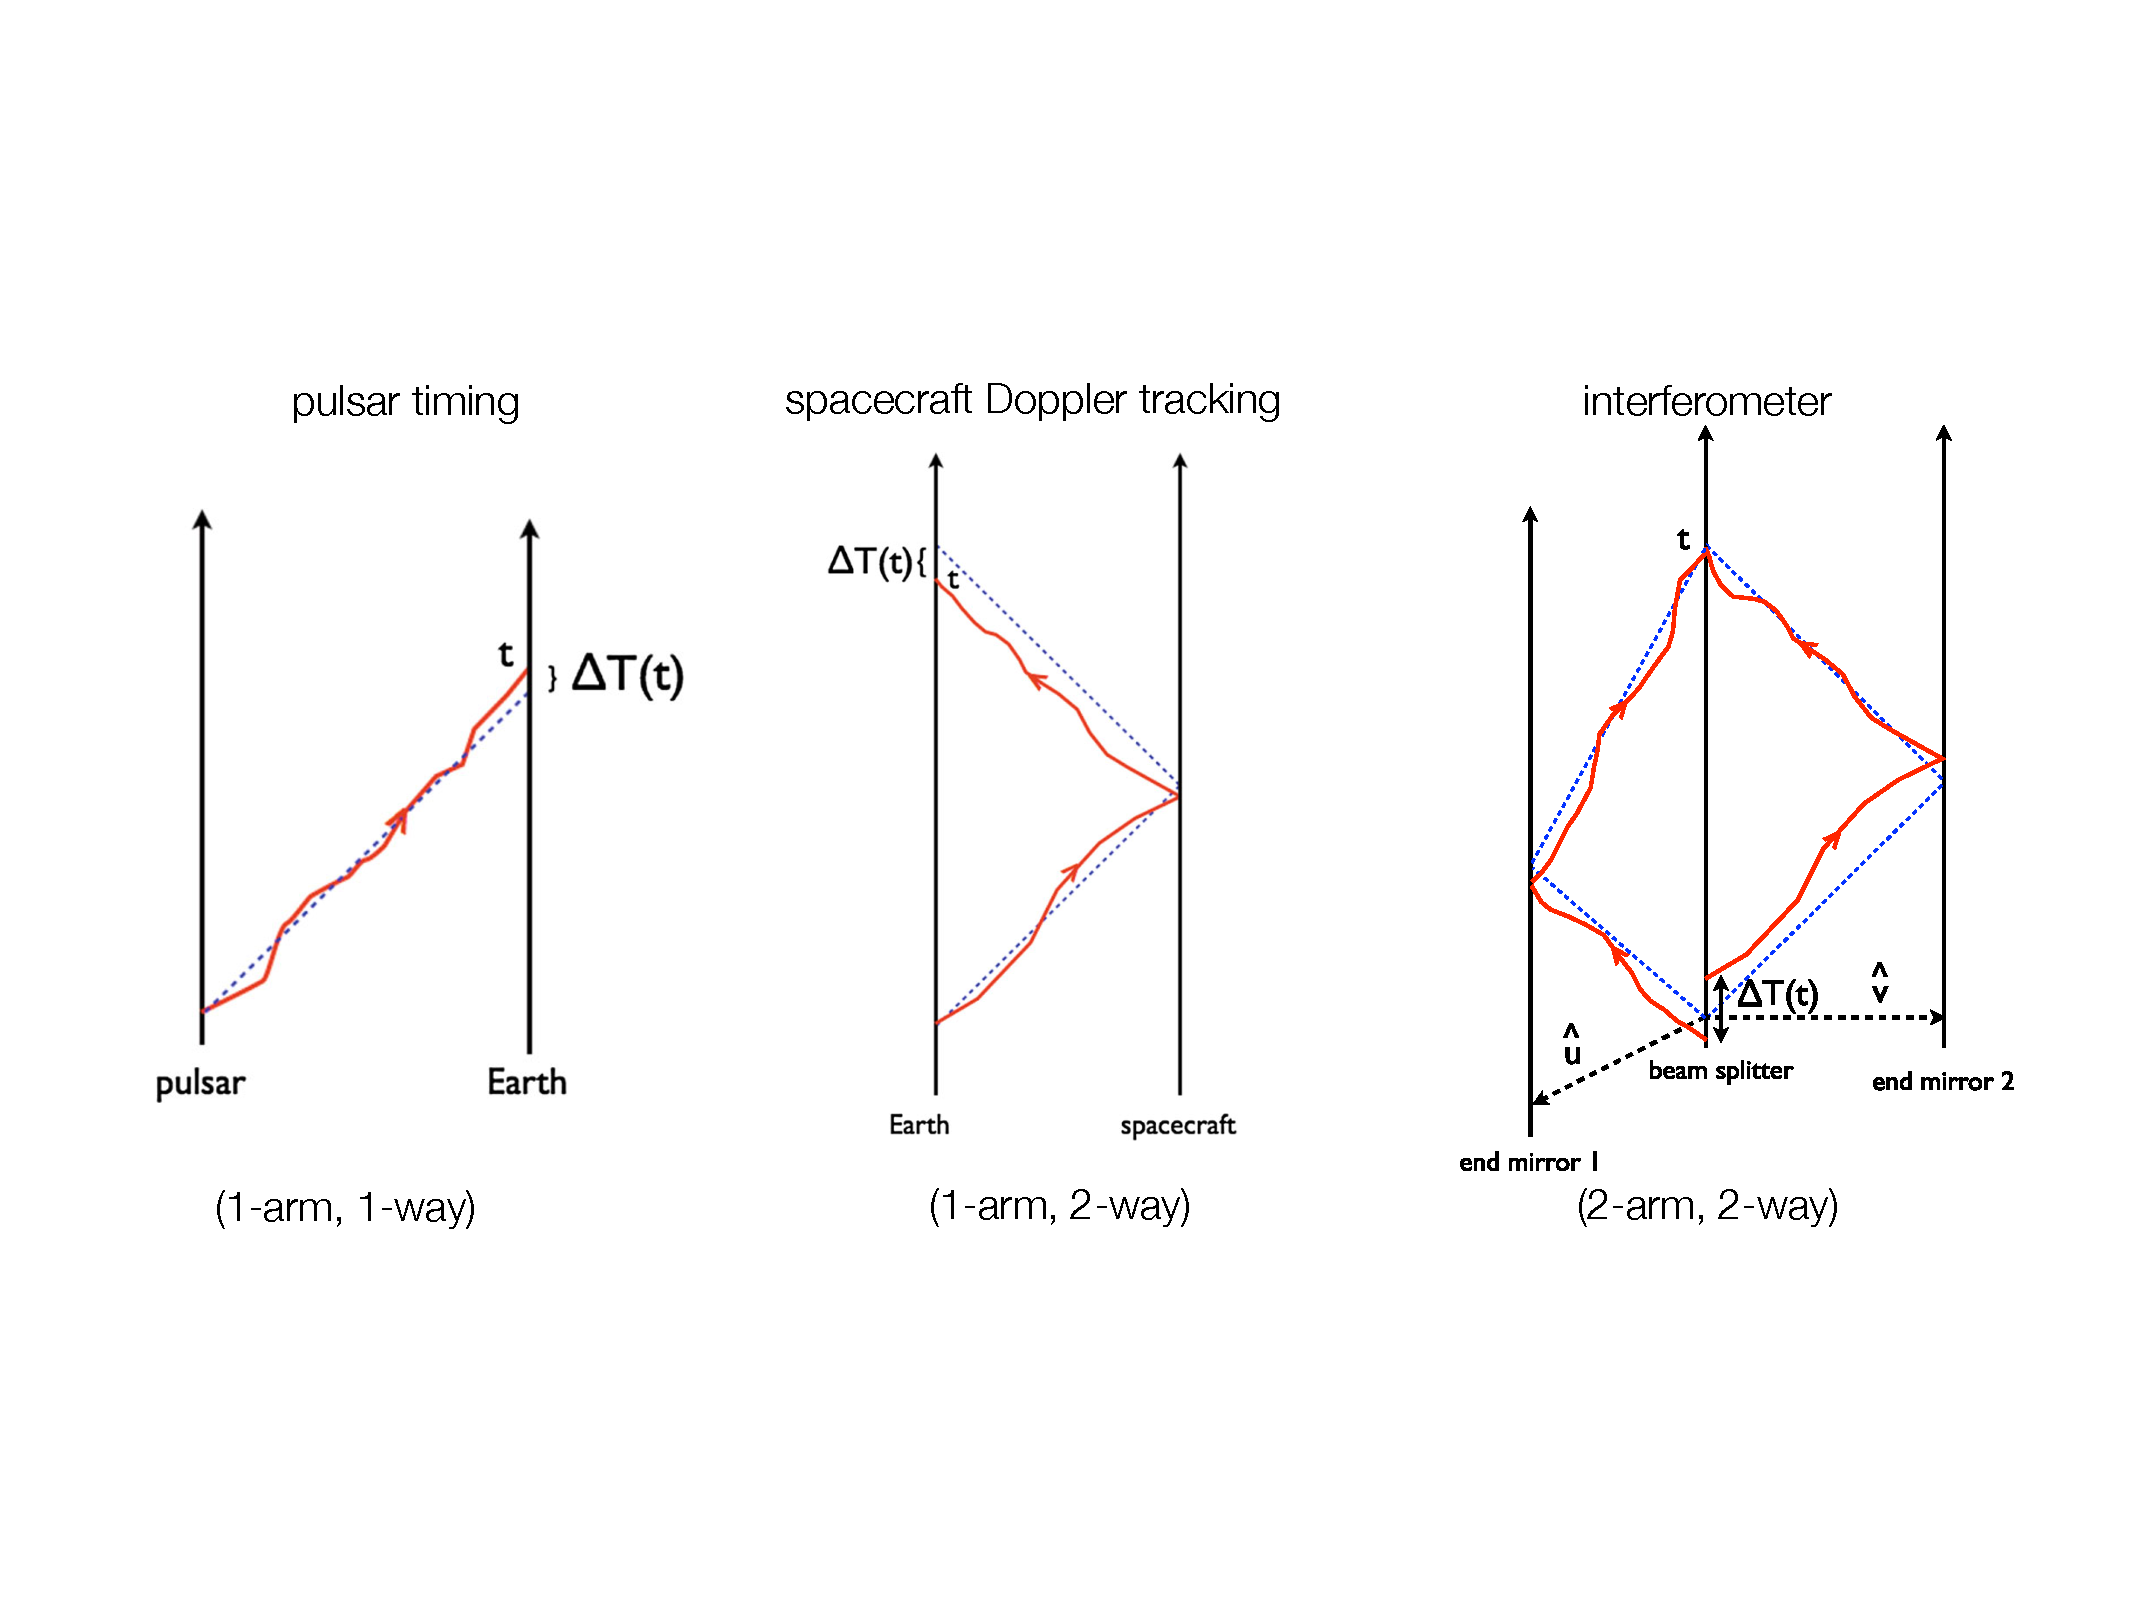
\includegraphics[width=\textwidth]{Figures/beam_detectors}
\caption{Spacetime diagram showing the response of beam
detectors to a passing GW.  
Left column: pulsar timing; middle column: spacecraft Doppler
tracking; right column: interferometer (ground or space-based).
A passing GW perturbs the path of the photon (red trajectory) 
relative to its nominal path in the absence of the wave 
(blue dotted line), leading to a 
difference in the expected arrival time of the photon.
(Figure adapted from \cite{Romano-Cornish:2017}.)}
\label{f:beam_detectors}
\end{center}
\end{figure}
%

In the literature, one might see the detector response
written in terms of strain $\Delta L(t)/L$, 
fractional Doppler frequency $\Delta v(t)/\nu_0$, or 
phase $\Delta\Phi(t)$, instead of the timing residual
$\Delta T(t)$.
Despite the apparent differences in the responses, 
they are all derivable from the change in light travel
time $\Delta T(t)$ via the relations:
%
\be
\begin{aligned}
&h(t)\equiv \Delta T(t)\quad &({\rm pulsar\ timing})\\
&h(t)\equiv \frac{\Delta L(t)}{L} = \frac{\Delta T(t)}{T}
\quad&({\rm LIGO,\ Virgo,\ }\cdots) \\
&h(t)\equiv \frac{\Delta\nu(t)}{\nu_0}=\frac{\D \Delta T(t)}{\D t}
\quad &({\rm spacecraft Doppler\ tracking})\\
&h(t)\equiv \Delta\Phi(t) = 2\pi \nu_0\,\Delta T(t)
\quad &({\rm LISA})\,.
\end{aligned}
\ee
%
Hence, once we know how to calculate the timing residual
response $\Delta T(t)$, we can easily calculate all the
other quantities listed above.

\subsection{Detector response functions}
\label{e:det_response}

GWs are weak.
As such, a detector act like a {\em linear} system, 
which converts metric perturbations to detector output.
Mathematically, this is represented by the 
{\em convolution} of the metric perturbations with the 
{\em response function} of the detector:
%
\be
h(t) = (\mb{R}*\mb{h})(t,\vec x)\equiv
\int_{-\infty}^\infty {\rm d}\tau
\int {\rm d}^3 y\>
R^{ab}(\tau,\vec y)h_ab(t-\tau, \vec x-\vec y)
\ee
%
Here $h(t)$ is the output of the detector at time $t$.
The vector $\vec x$ is the location of detector, and 
$R^{ab}(\tau,\vec y)$ is the {\em impulse repsonse}
of the detector.
Expanding $h_{ab}(t-\tau,\vec x-\vec y)$ as a sum of
plane waves \eqref{e:planewave}, we find that the Fourier
transform $\tilde h(f)$ of $h(t)$ can be written as
%
\be
\tilde h(f)=\int {\rm d}^2\Omega_{\hat n}\sum_A R^A(f,\hat n)\,h_A(f,\hat n)
\ee
%
where
%
\be
R^A(f,\hat n) \equiv R^{ab}(f,\hat n)e^A_{ab}(\hat n)
\ee
%
and
%
\be
R^{ab}(f,\hat n) \equiv e^{i 2\pi f\hat n\cdot\vec x/c}\,
\int_{-\infty}^\infty {\rm d}\tau \int {\rm d}^3 y\>
R^{ab}(\tau,\vec y)\,e^{-i2\pi f(\tau+\hat n\cdot\vec y/c)}
\ee
%
Note that $R^A(f,\hat n)$ is the 
detector response for a plane-wave
with frequency $f$, propagation direction $\hat k$, and polarization $A$.

\subsection{Examples}

\subsubsection{Detector response for a one-arm, one-way detector}

For our first example, we will consider the timing response of a one-arm,
one-way beam detector, which is relevant for pulsar timing observations.
The geometry of the situation is shown in Figure~\ref{f:one_arm_one_way}.
%
\begin{figure}[htbp!]
\begin{center}
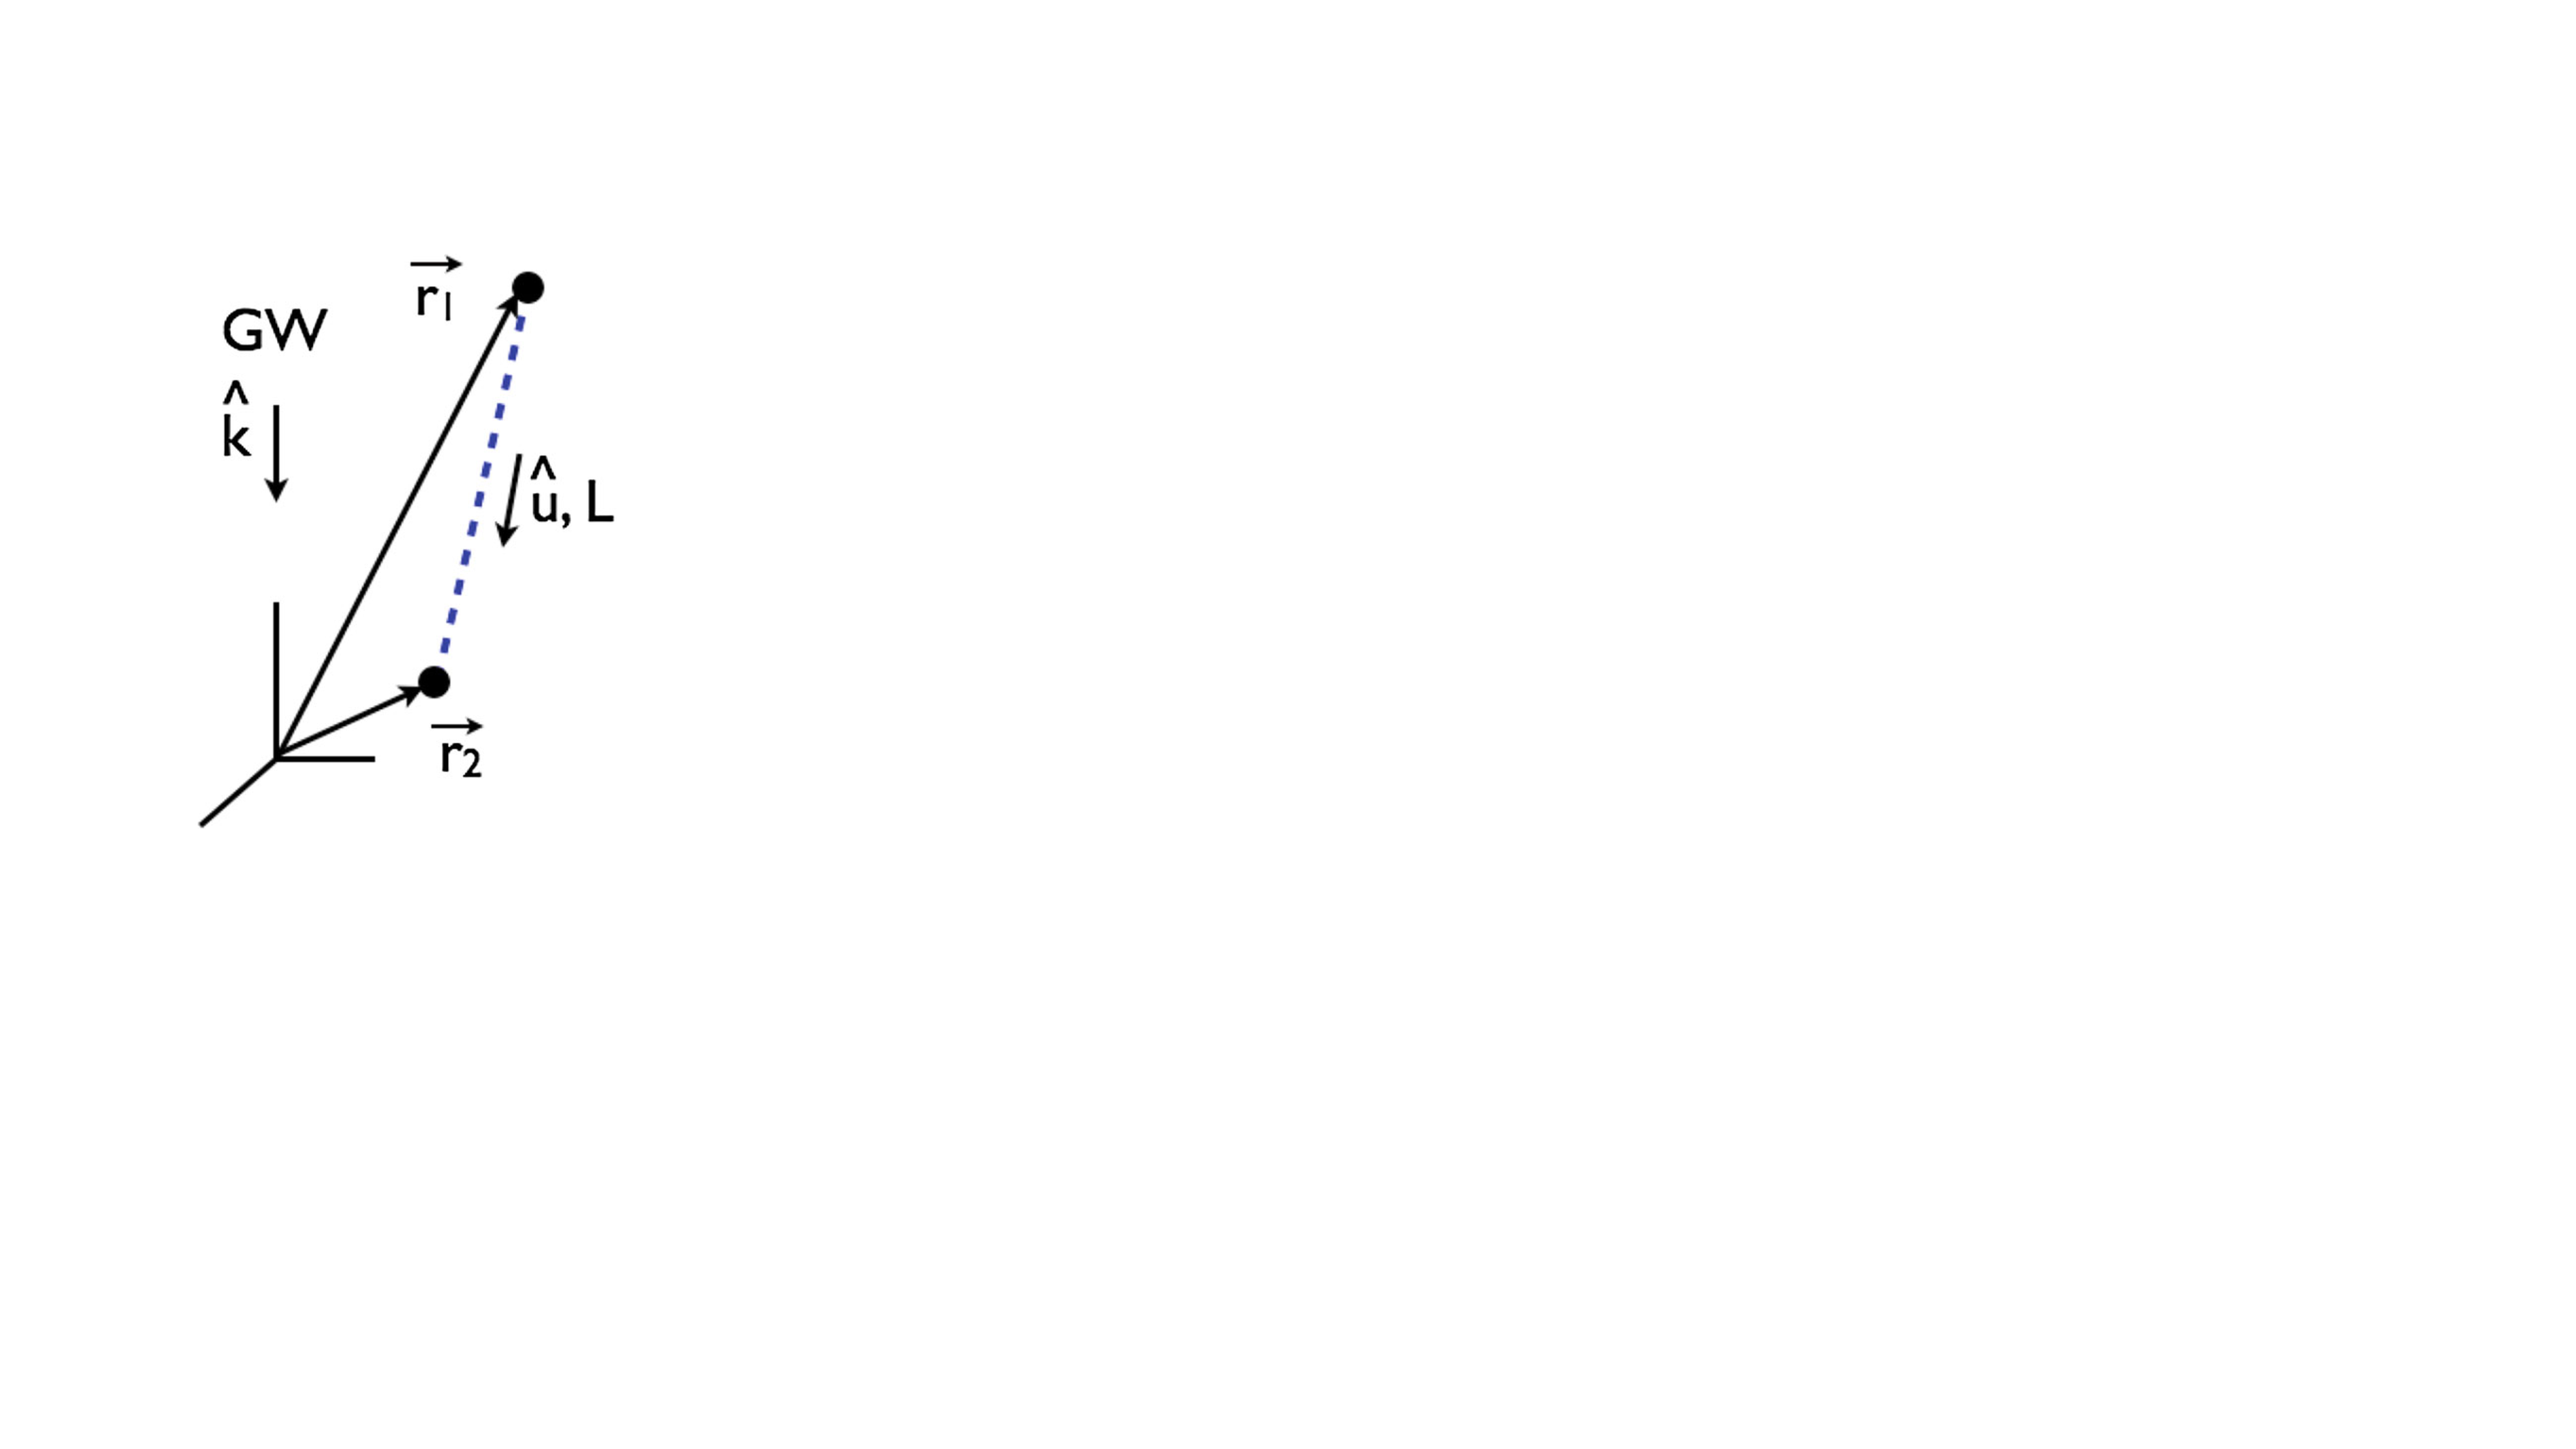
\includegraphics[width=0.2\textwidth]{Figures/one_arm_one_way}
\caption{Geometry for a one-arm, one-way beam detector, relevant for 
a pulsar timing residual measurement.
The GW propagates in the $\hat k$ direction; the electromagnetic wave
(e.g., a radio pulse from a pulsar) propagates in the $\hat u$ direction
(opposite of the direction to the pulsar, $\hat p=-\hat u$.} 
\label{f:one_arm_one_way}
\end{center}
\end{figure}
%
\be
h(t)\equiv
\Delta T(t) = \frac{1}{2c} u^a u^b\int_0^L{\rm d}s\> h_{ab}(t(s),\vec x(s))
\ee
%
%
\be
t(s) = (t-L/c) + s/c\,, \qquad
\vec x(s) = \vec r_1 + s\hat u
\ee
%
In Exercise 6, you are asked to show that the timing
residual response is given by
%
\be
R^A(f,\hat n) = \frac{1}{i2\pi f}\,
\frac{1}{2}u^a u^b e^A_{ab}(\hat n)\frac{1}{1+\hat n\cdot \hat u}\,
\left[ 1-e^{-\frac{i 2\pi fL}{c}(1+\hat n\cdot\hat u)}\right]
\,e^{i2\pi f\hat n\cdot\vec r_2/c}
\ee
%
In the context of pulsar timing, the two terms in square brackets 
are called the {\em Earth term} and {\em pulsar term} respectively.
The pulsar term encodes information about the phase of the GW at
the location of the pulsar.
It is usually ignored for stochastic background searches, as 
this term for different pulsars will not be correlated with one other
(since the spatial distance between two pulsars is much greater than
the wavelengths of the GWs that pulsar timing arrays are 
sensitive to).

Note that the factor $1/(i2\pi f)$ goes away for the Doppler 
frequency response, $\Delta\nu(t)/\nu_0$, and that the
phase term $e^{-i2\pi f\hat k\cdot\vec r_2/c}$ equals one
if we take the $\vec r_2$ to be the origin of coordinates, e.g.,
at the solar system barycentre.
Then the Doppler frequency response simplifies to 
%
\be
F^A(\hat k) 
=\frac{1}{2}u^a u^b e_{ab}^A(\hat k)\frac{1}{1-\hat k\cdot\hat u}
\label{e:F^A(k)}
\ee
%
where the last expression is written in terms of the direction
to the pulsar $\hat p = -\hat u$.
A plot of this response, summed over the two polarizations,
is shown in Figure~\ref{f:one_arm_one_way_peanut}.
%
\begin{figure}[htbp!]
\begin{center}
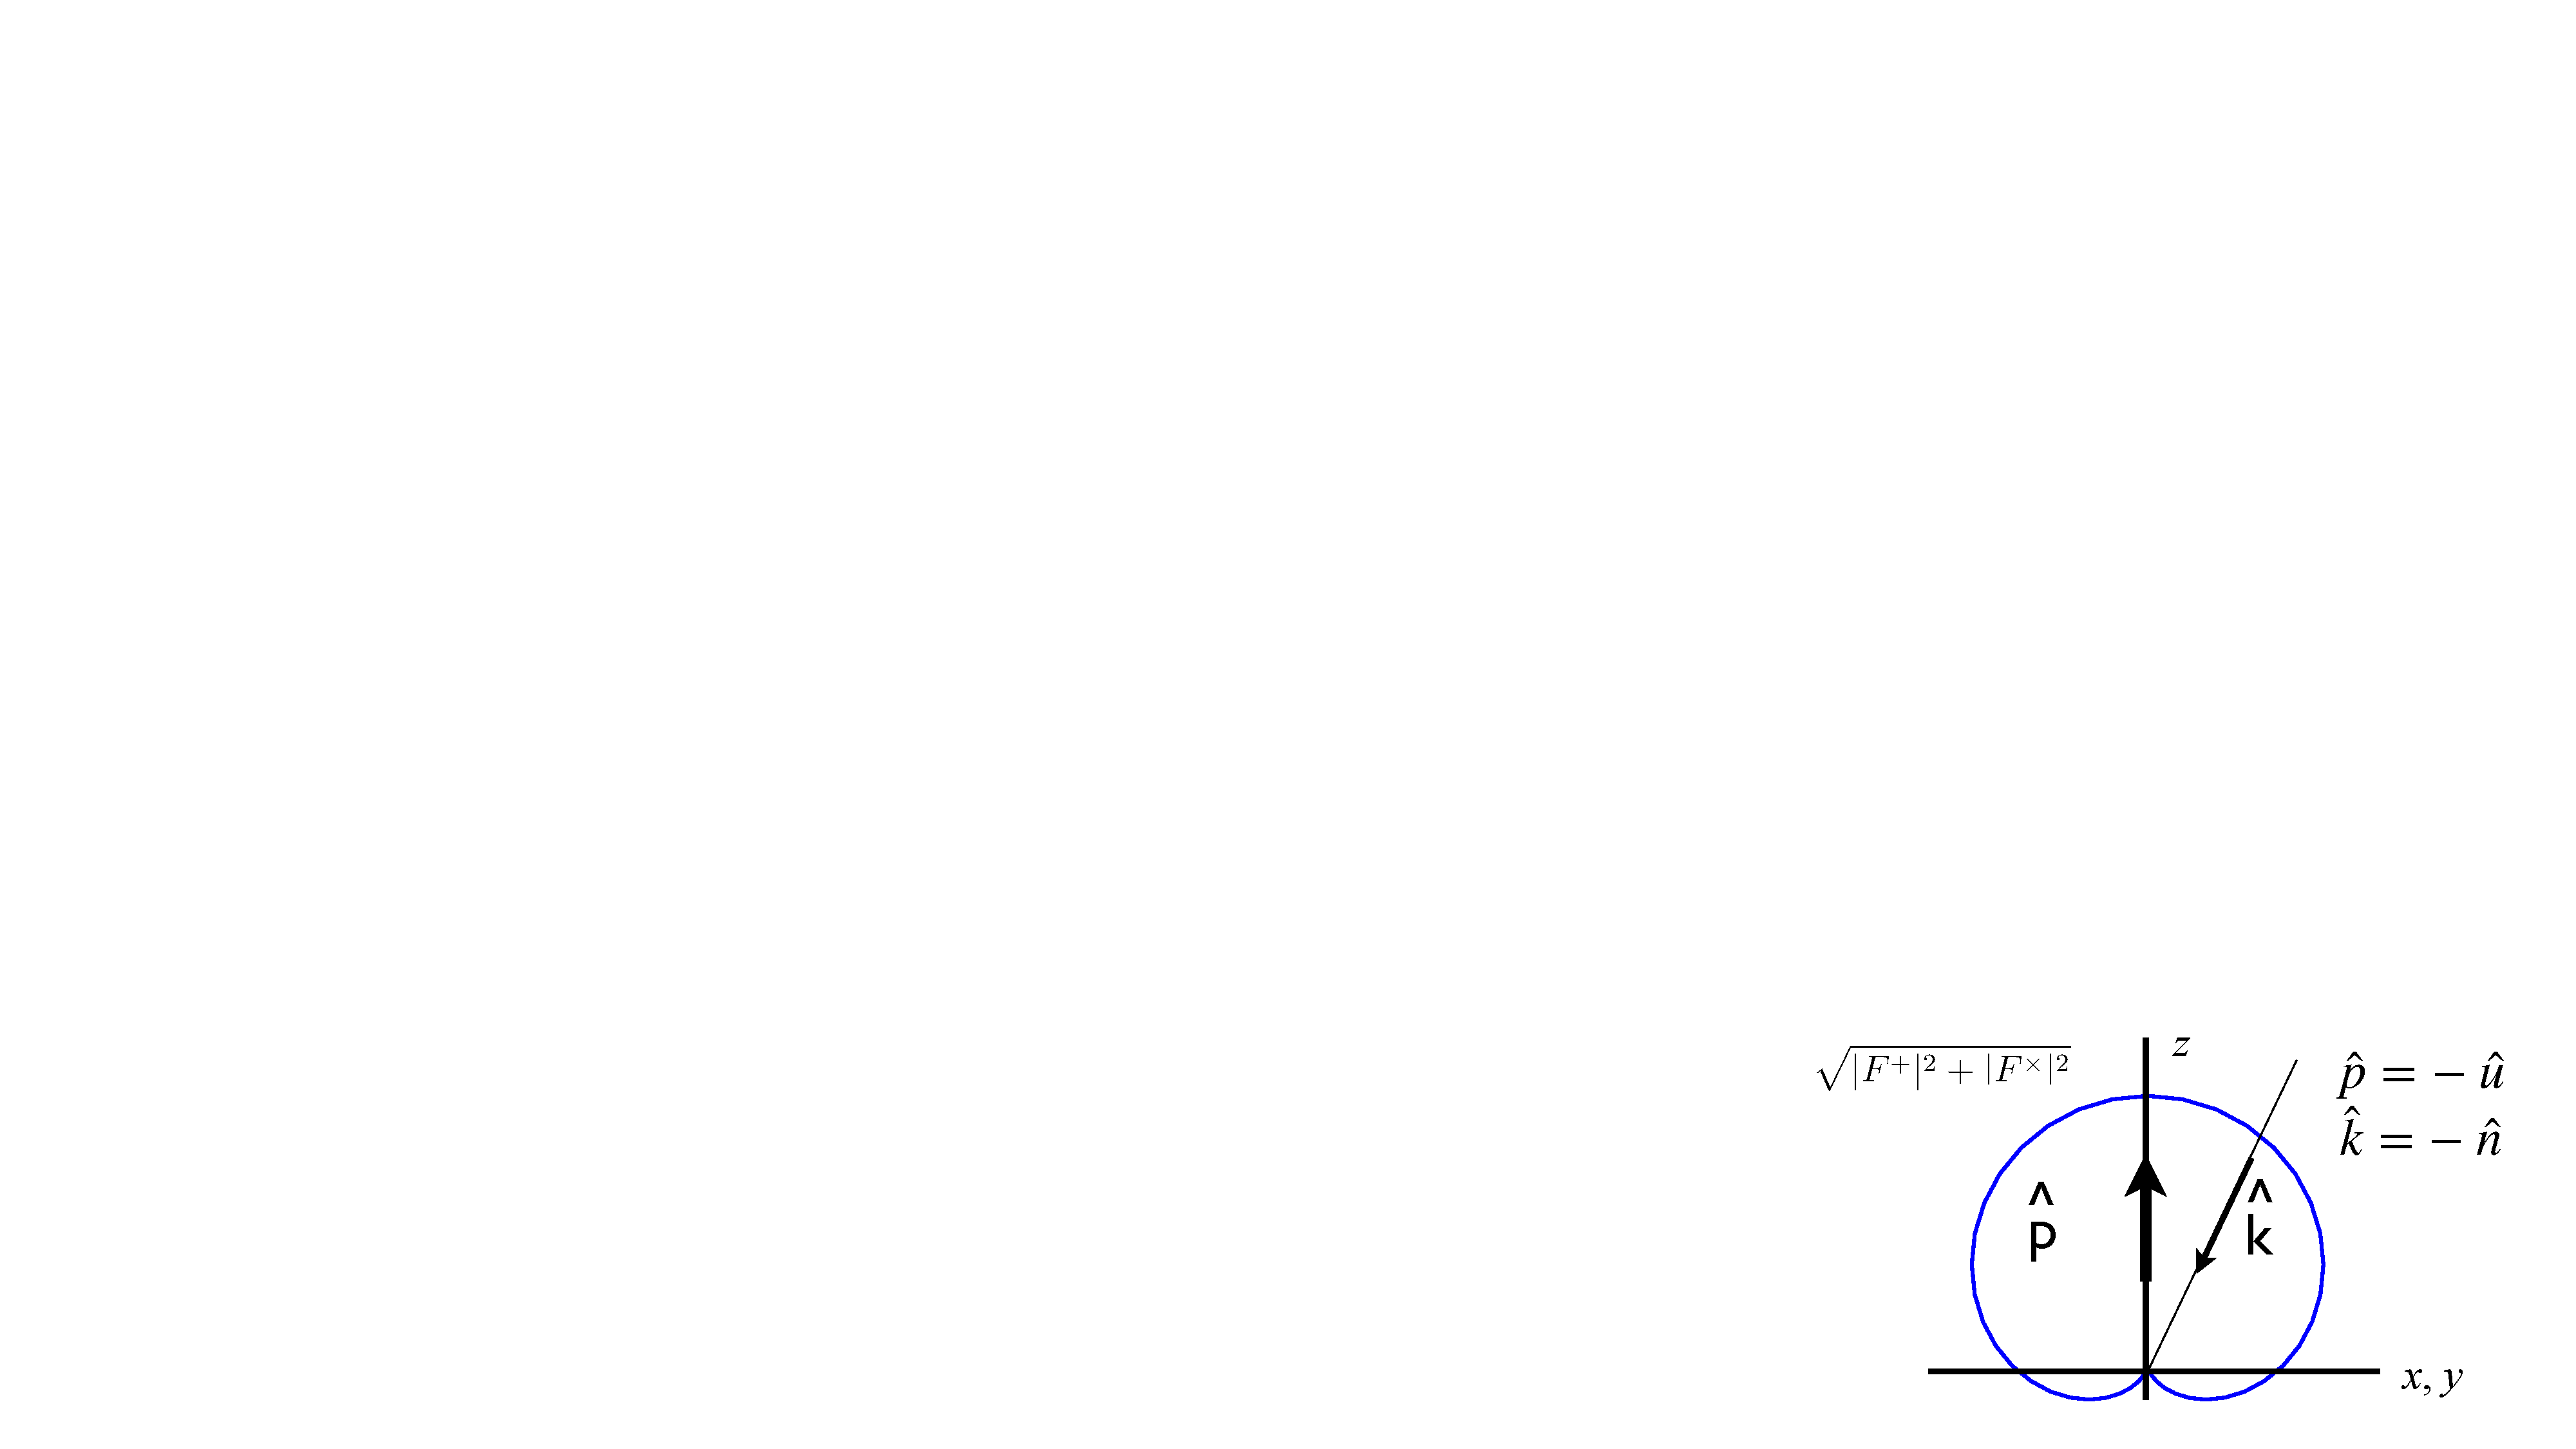
\includegraphics[width=0.4\textwidth]{Figures/one_arm_one_way_peanut}
\caption{Polarization-averaged Doppler frequency response
$\sqrt{|F^+(\hat k)|^2+|F_\times(\hat k)|^2}$
for pulsar timing, ignoring the frequency-dependendent part of
the pulsar term.
The response is axially symmetric around the $z$-axis, which
we've chose to be the direction to the pulsar $\hat p=-\hat u$.}
\label{f:one_arm_one_way_peanut}
\end{center}
\end{figure}
%
The response is maximum when the GW and radio pulse propagate 
in the same direction---i.e., when $\hat k=\hat u$.
It is zero when they propagate in opposite directions.
These results follow from 
%
\be
\begin{aligned}
&u^a u^b e^+_{ab}(\hat k) 
= \sin^2\theta = (1-\cos\theta)(1+\cos\theta)\,,
\\
&u^a u^b e^\times_{ab}(\hat k)=0\,,
\end{aligned}
\ee
%
and
%
\be
\frac{1}{1-\hat k\cdot\hat u} = \frac{1}{1-\cos\theta}\,,
\ee
%
where $\hat u=-\hat z$ and $\theta$ is the usual polar
angle between $\hat k$ and the $z$ direction.

%%%%%%%%%%%%%%%%%%%%%%%%%%%%%%
\subsubsection{Detector response for a laser interferometer 
in the short-antenna limit}

Another simple example of a detector response function is
for a equal-arm laser interferometer, like LIGO, in the 
{\em short-antenna limit} (Figure~\ref{f:LHO_geometry}).
%
\begin{figure}[htbp!]
\begin{center}
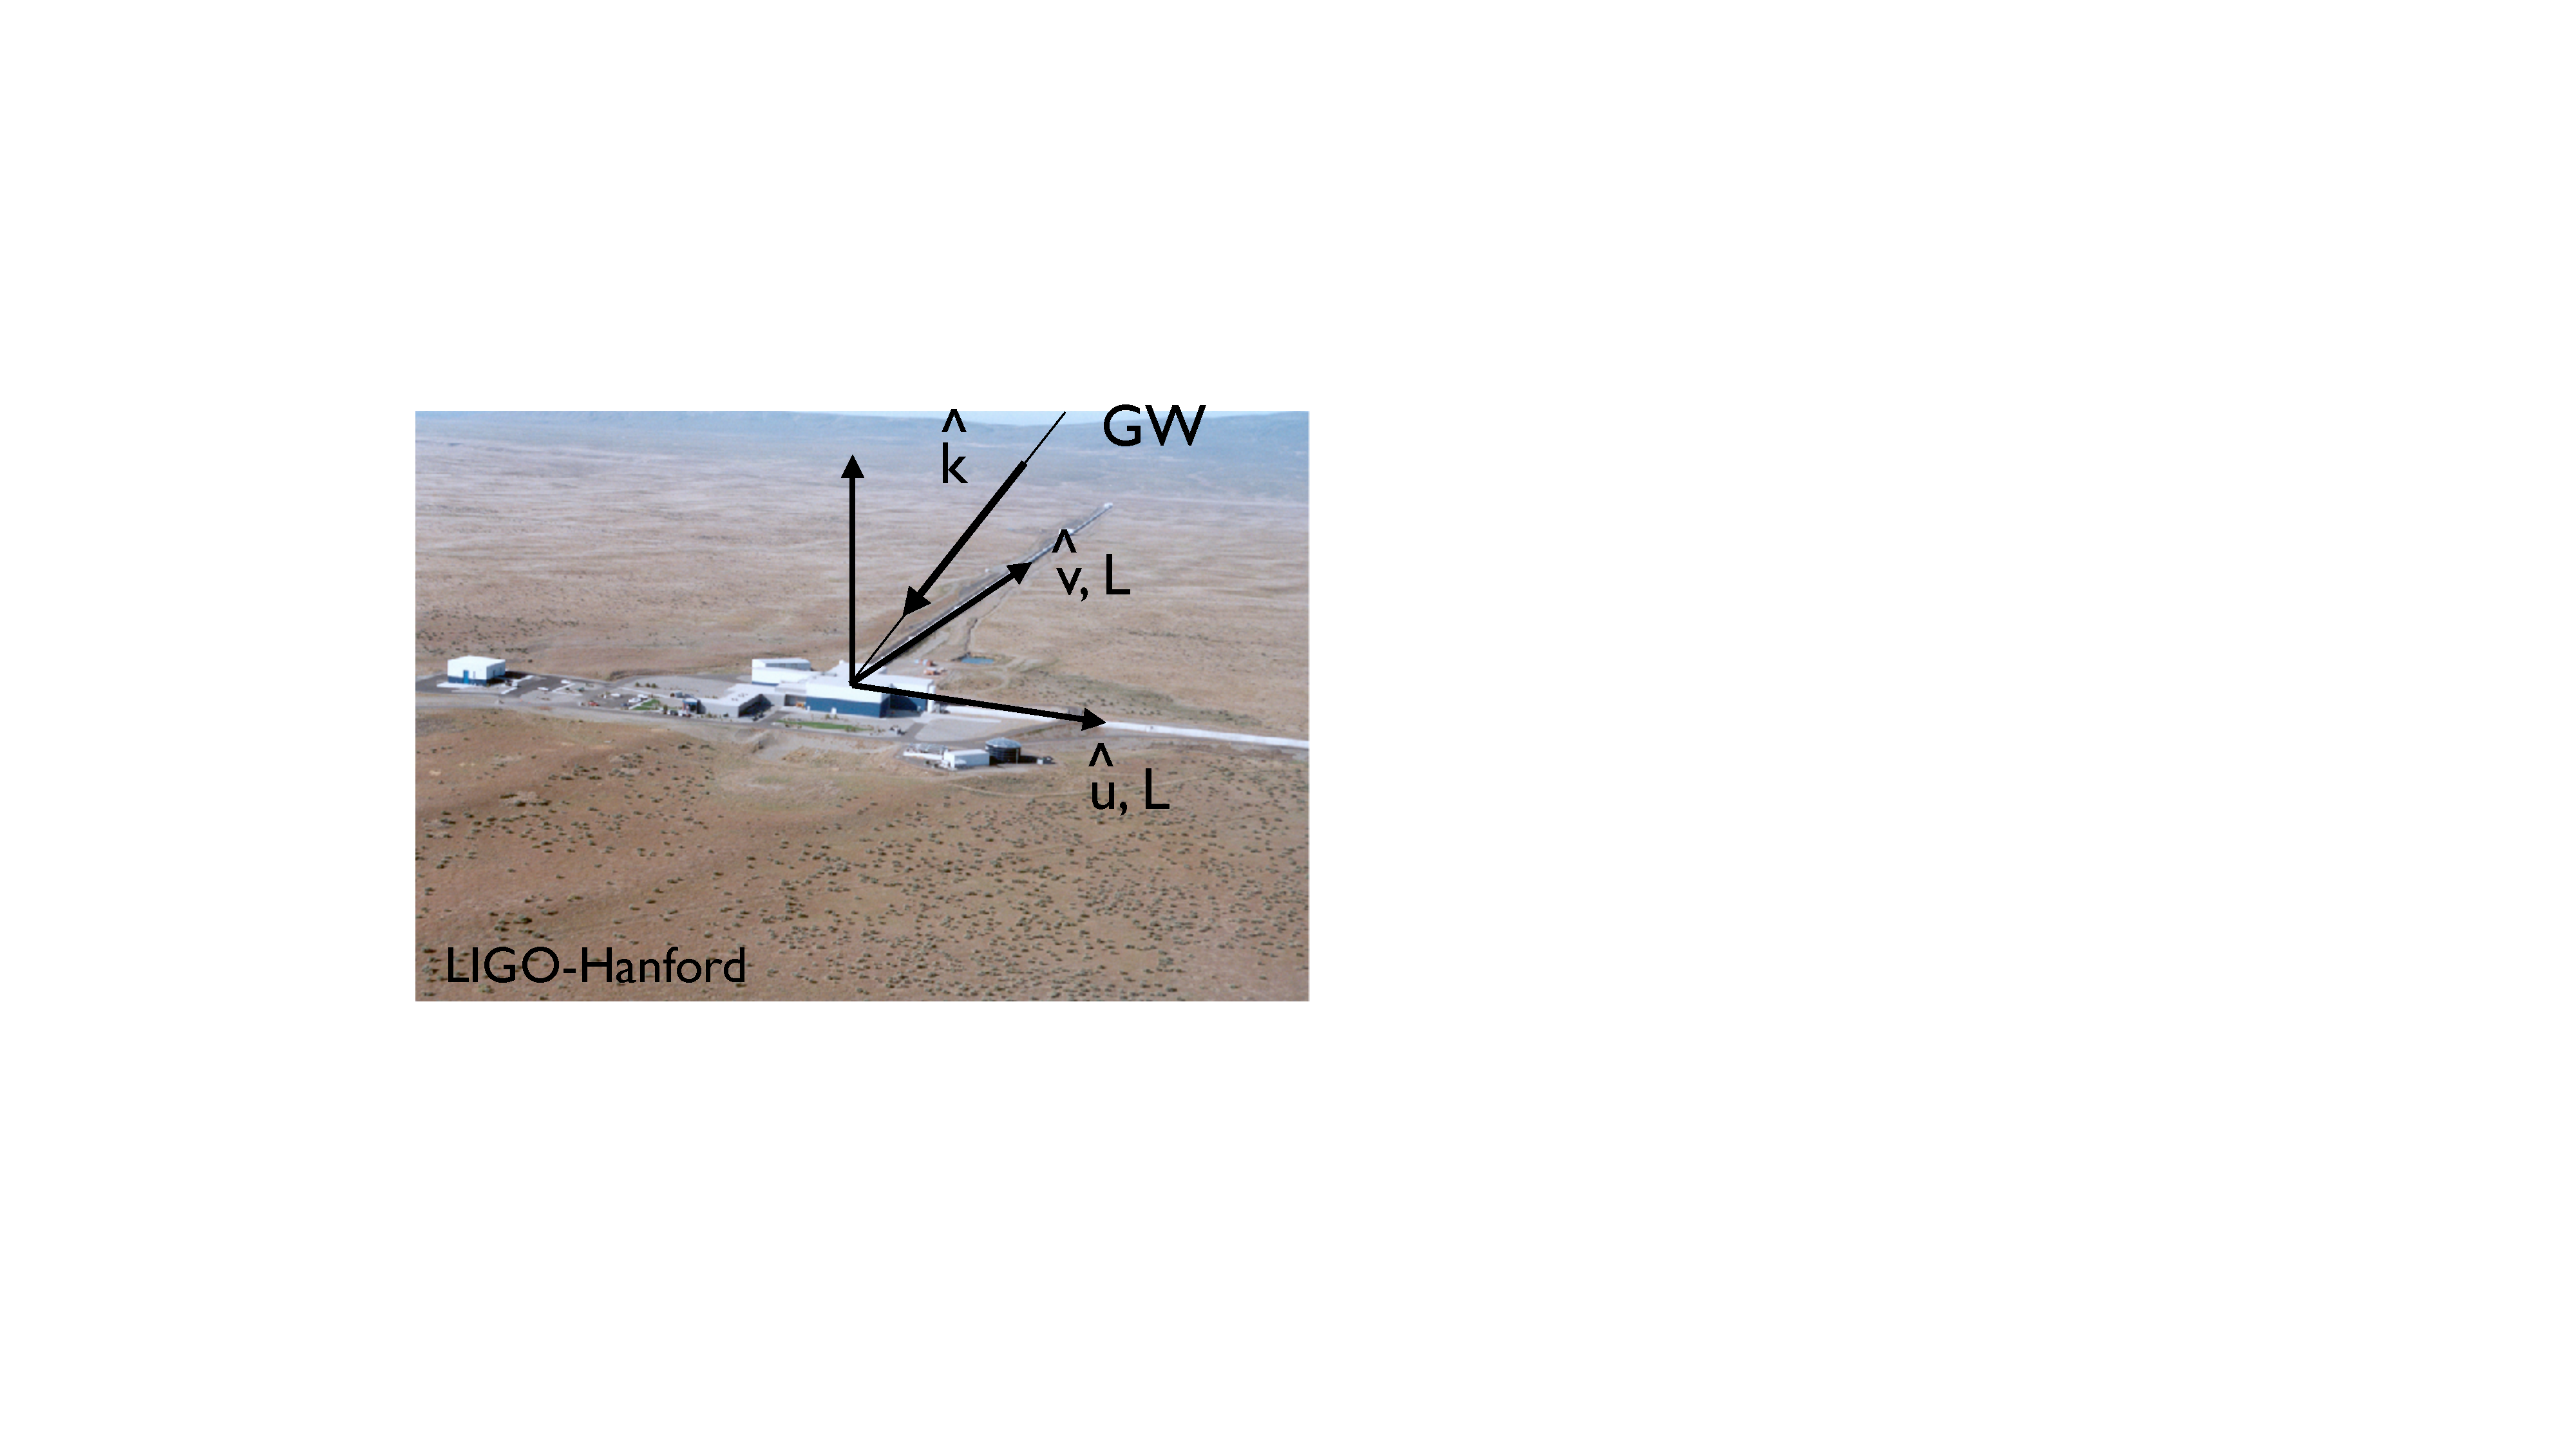
\includegraphics[width=0.6\textwidth]{Figures/LHO_geometry}
\caption{Geometry for a ground-based interferometer GW response
calculation.
(Shown here the LIGO Hanford Observatory, in Hanford, WA.)
The GW propagates in the $\hat k$ direction;
$\hat u$, $\hat v$ are unit vectors that point along the 
two arms of the interferometer.
In the short-antenna approximation, the length $L$ of the 
arms does not enter the expression for the response function.}
\label{f:LHO_geometry}
\end{center}
\end{figure}
%
This approximation is valid when the wavelength of the GW is 
much larger than the dimensions of the detector.  
Then, the GW phase is effectively constant as a photon
travels down an back an interferometer arm.
Defining the strain response of the interferometer as
%
\be
h(t) = \frac{1}{2}\left(
\frac{\Delta T_{\vec u,\, {\rm roundtrip}}(t)}{T}
-
\frac{\Delta T_{\vec v,\, {\rm roundtrip}}(t)}{T}
\right)
\ee
%
one can show that
%
\be
R^A(f,\hat n)\simeq\frac{1}{2}\left(u^au^b-v^av^b\right)\,e^A_{ab}(\hat n)
\ee
%
The quantity multiply $e^A_{ab}(\hat k)$ in the 
reponse function
is called the {\em detector tensor}
%
\be
D^{ab}\equiv\frac{1}{2}\left(u^a u^b - v^a v^b\right)\,.
\ee
%
Plots of the {\em beam pattern functions}
$|R^+(f,\hat k)|$, $|R^\times(f,\hat k)|$ for the 
two polarizations individually, and the 
root-summed-squared response for both polarization
$\sqrt{|R^+(f,\hat k)|^2 + |R^\times(f,\hat k)|^2}$
is shown in Figure~\ref{f:LIGO_beam_patterns}.
%
\begin{figure}[htbp!]
\begin{center}
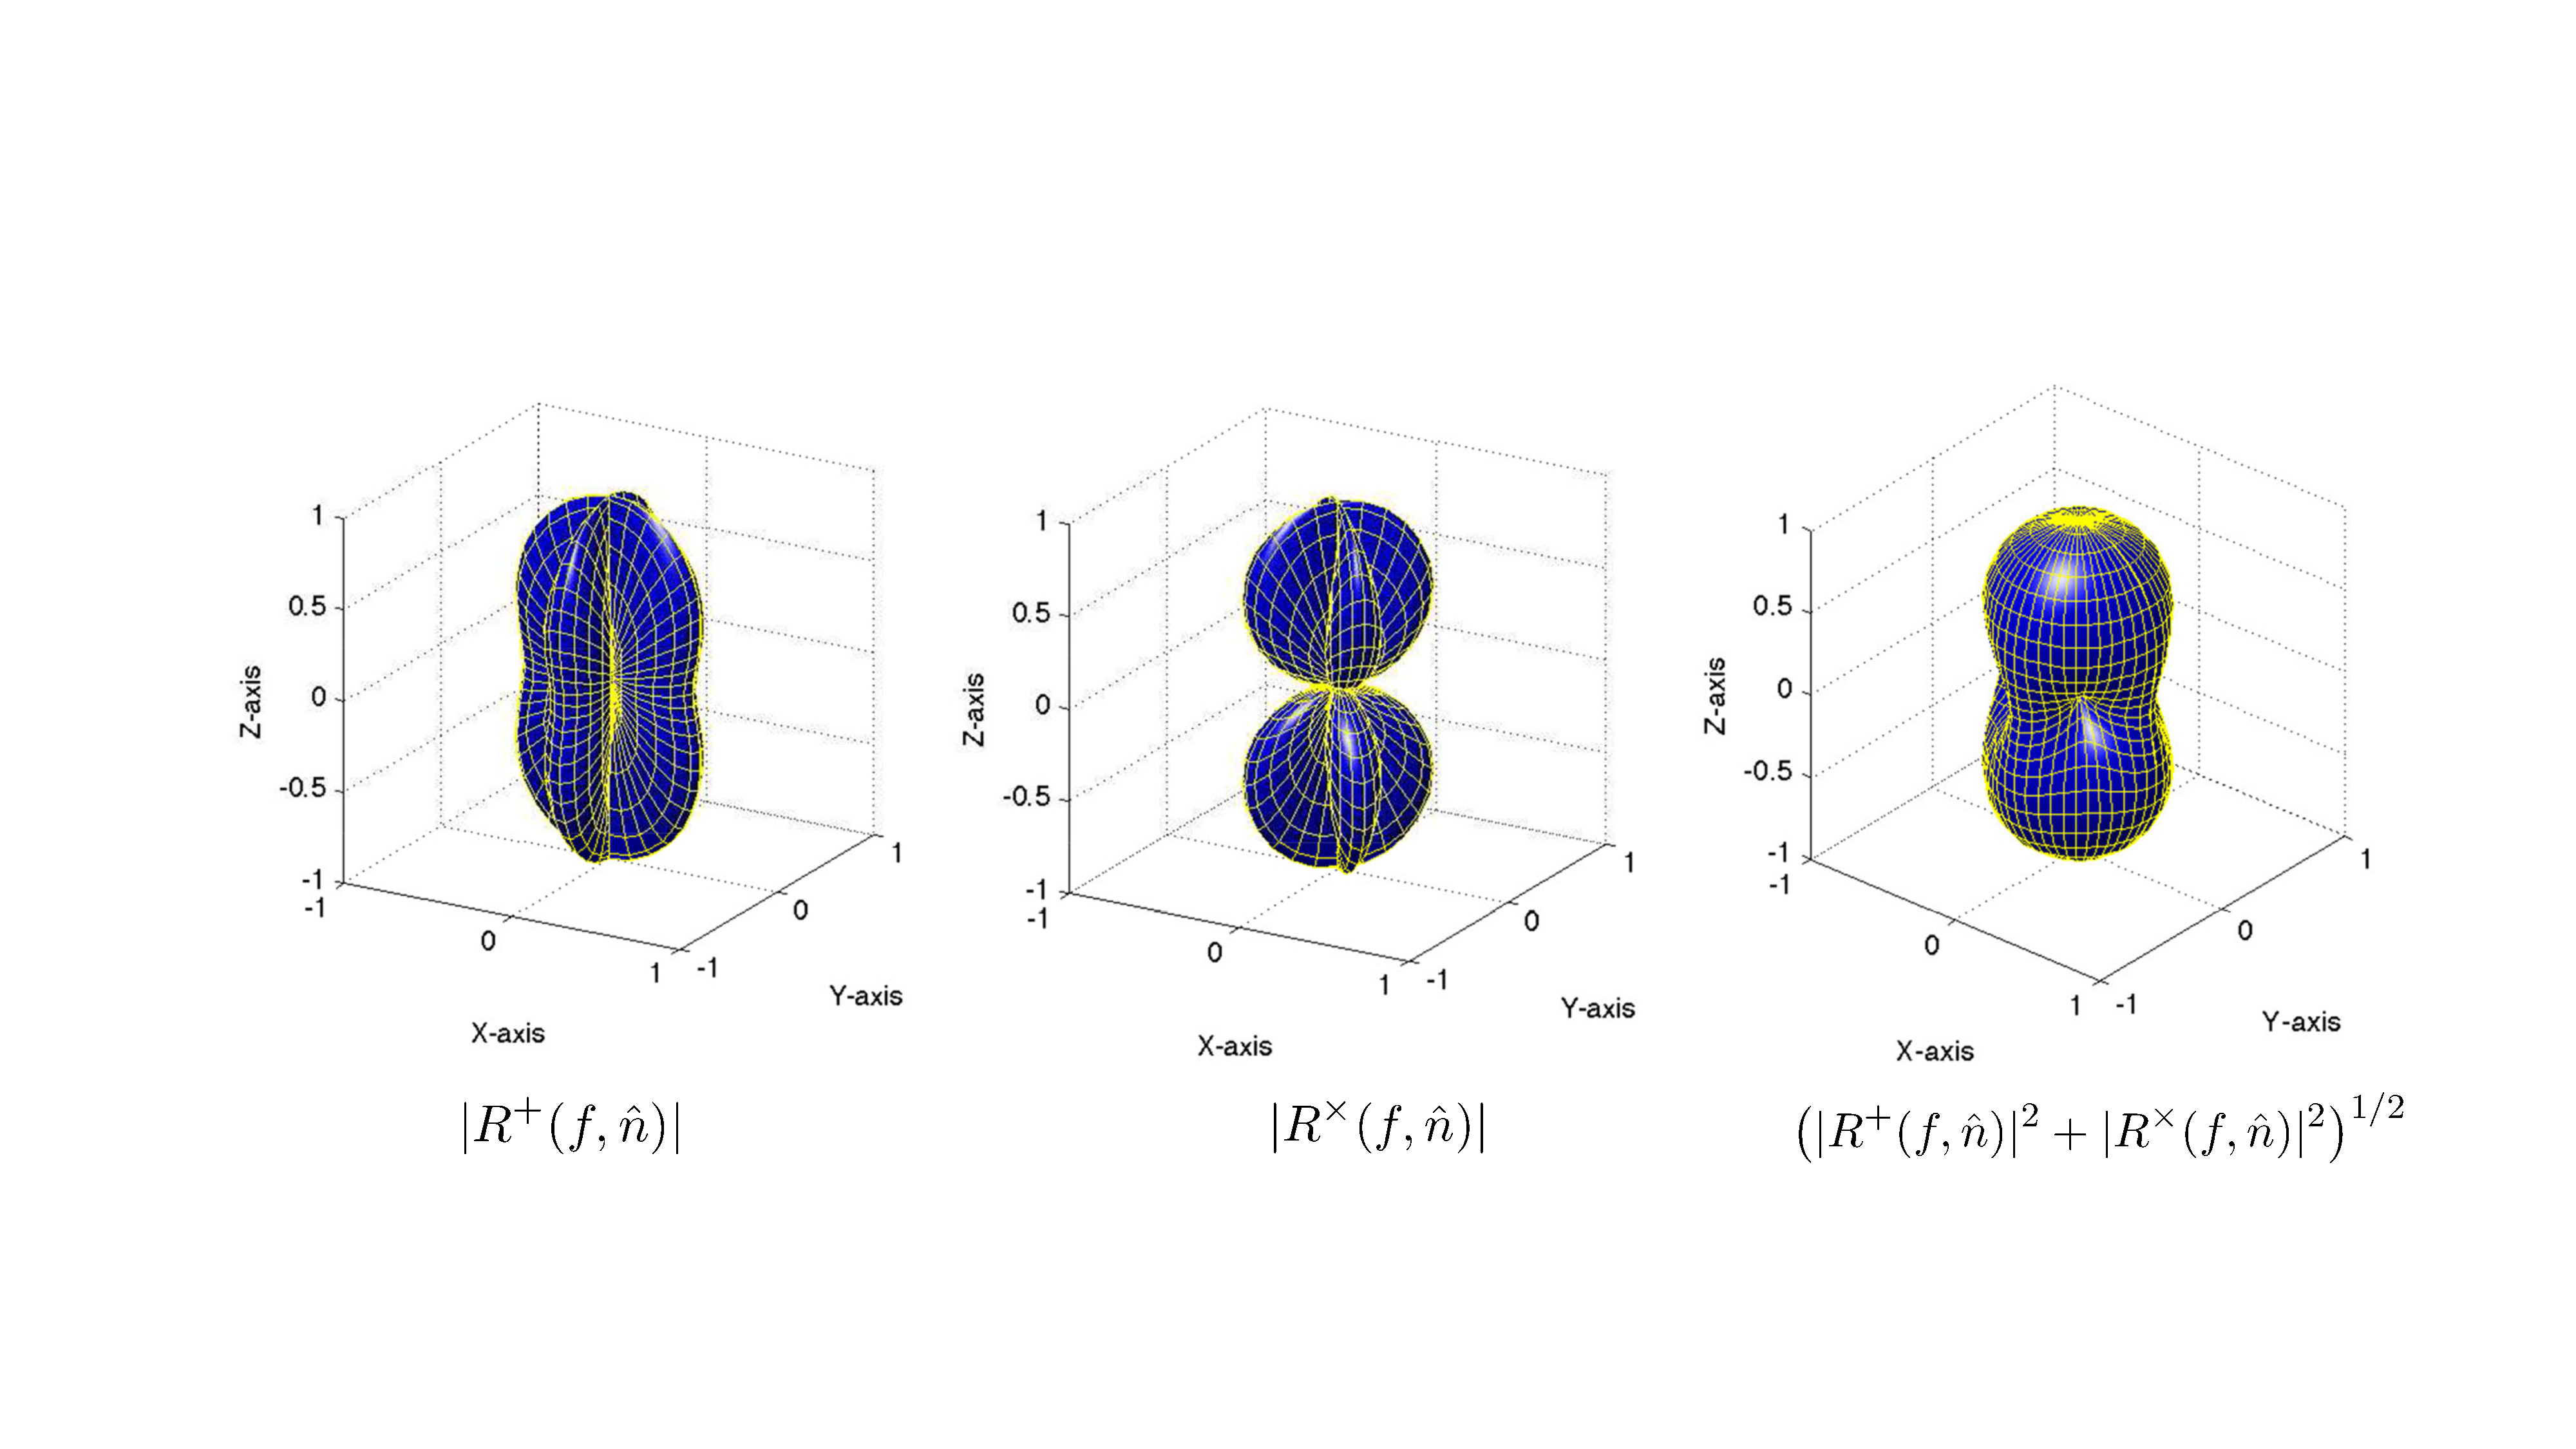
\includegraphics[width=\textwidth]{Figures/LIGO_beam_patterns}
\caption{Beam pattern functions for a ground-based interferometer
like LIGO in the short-antenna approximation---i.e., $f\lesssim {\rm few\ kHz}$.
The vertex of the interferometer is at the origin of coordinates,
and interferometer arms are assumed to be orthogonal pointing along
the $x$ and $y$ directions.}
\label{f:LIGO_beam_patterns}
\end{center}
\end{figure}

%%%%%%%%%%%%%%%%%%%%%%%%%%%%%%%%%%%%%%%%%%%%%%%%%%%%%%
\section{Non-trivial correlations}
\label{s:nontrivial_correlations}

\subsection{Overlap function}

Detectors in different locations and with different 
orientations respond differently to a passing GW.
Overlap function encodes reduction in sensitivity of a
cross-correlation analysis due to separation and misalignment 
of the detectors.

In the time domain:
%
\be
\langle h_I(t)h_J(t')\rangle 
= \frac{1}{2}\int_{-\infty}^\infty{\rm d}f\>
e^{i2\pi f(t-t')}\Gamma_{IJ}(f)S_h(f)
\label{e:Gamma-time}
\ee
%
In the frequency domain:
%
\be
\langle \tilde h_I(f)\tilde h_J^*(f')\rangle 
= \frac{1}{2}\delta(f-f')\Gamma_{IJ}(f)S_h(f)
\label{e:Gamma-freq}
\ee
%
One finds
%
\be
\Gamma_{IJ}(f) 
= \frac{1}{8\pi}\int {\rm d}^2\Omega_{\hat n}\> 
\sum_A R_I^A(f,\hat n) R_J^{A}{}^{*}(f,\hat n)
\label{e:Gamma}
\ee
%
for an unpolarized, stationary isotropic GWB.
As mentioned in Section~\ref{s:optimal_filtering},
$\Gamma_{IJ}(f)$ is the transfer function between the strain
power in the GWB and detector cross-power.
The integrand of $\Gamma_{IJ}(f)$ is important for 
statistically {\em anisotropic} backgrounds as the 
right-hand-side of \eqref{e:Gamma-freq} is replaced by
%
\be
\frac{1}{8\pi}\int {\rm d}^2\Omega_{\hat k}\> 
\sum_A R_I^A(f,\hat k) R_J^{A}{}^{*}(f,\hat k) {\cal P}(f,\hat k)
\label{e:aniso_RHS}
\ee
%
One then typically expands 
${\cal P}(f,\hat k)$ in terms of spherical harmonics 
%
\be
{\cal P}(f,\hat k) = \sum_{l=0}^\infty\sum_{m=-l}^l
{\cal P}_{lm}(f)Y_{lm}(\hat k)\,,
\ee
%
for which \eqref{e:Gamma-freq} becomes
%
\be
\langle \tilde h_I(f)\tilde h_J^*(f')\rangle 
= \frac{1}{2}\delta(f-f')\sum_{l=0}^\infty\sum_{m=-l}^l
\Gamma_{IJ,lm}(f,\hat k){\cal P}_{lm}(f)\,.
\label{e:Gamma-freq}
\ee
%
with
%
\be
\Gamma_{IJ,lm}(f,\hat k) = 
\frac{1}{8\pi}
\sum_A R_I^A(f,\hat k) R_J^{A}{}^{*}(f,\hat k) 
Y_{lm}(\hat k)\,.
\ee
%
Interested readers can find much more discussion
about anisotropic background in Section~7 of
\cite{Romano-Cornish:2017}, and references to the
original work cited therein.

\subsection{Examples}

\subsubsection{Overlap function for a pair of laser
interferometers in the short-antenna limit}

Note that the first zero crossing occurs at roughly
60~Hz, corresponding to GW with wavelength equal to 
twice the separation between the two observatories.

\begin{figure}[htbp!]
\begin{center}
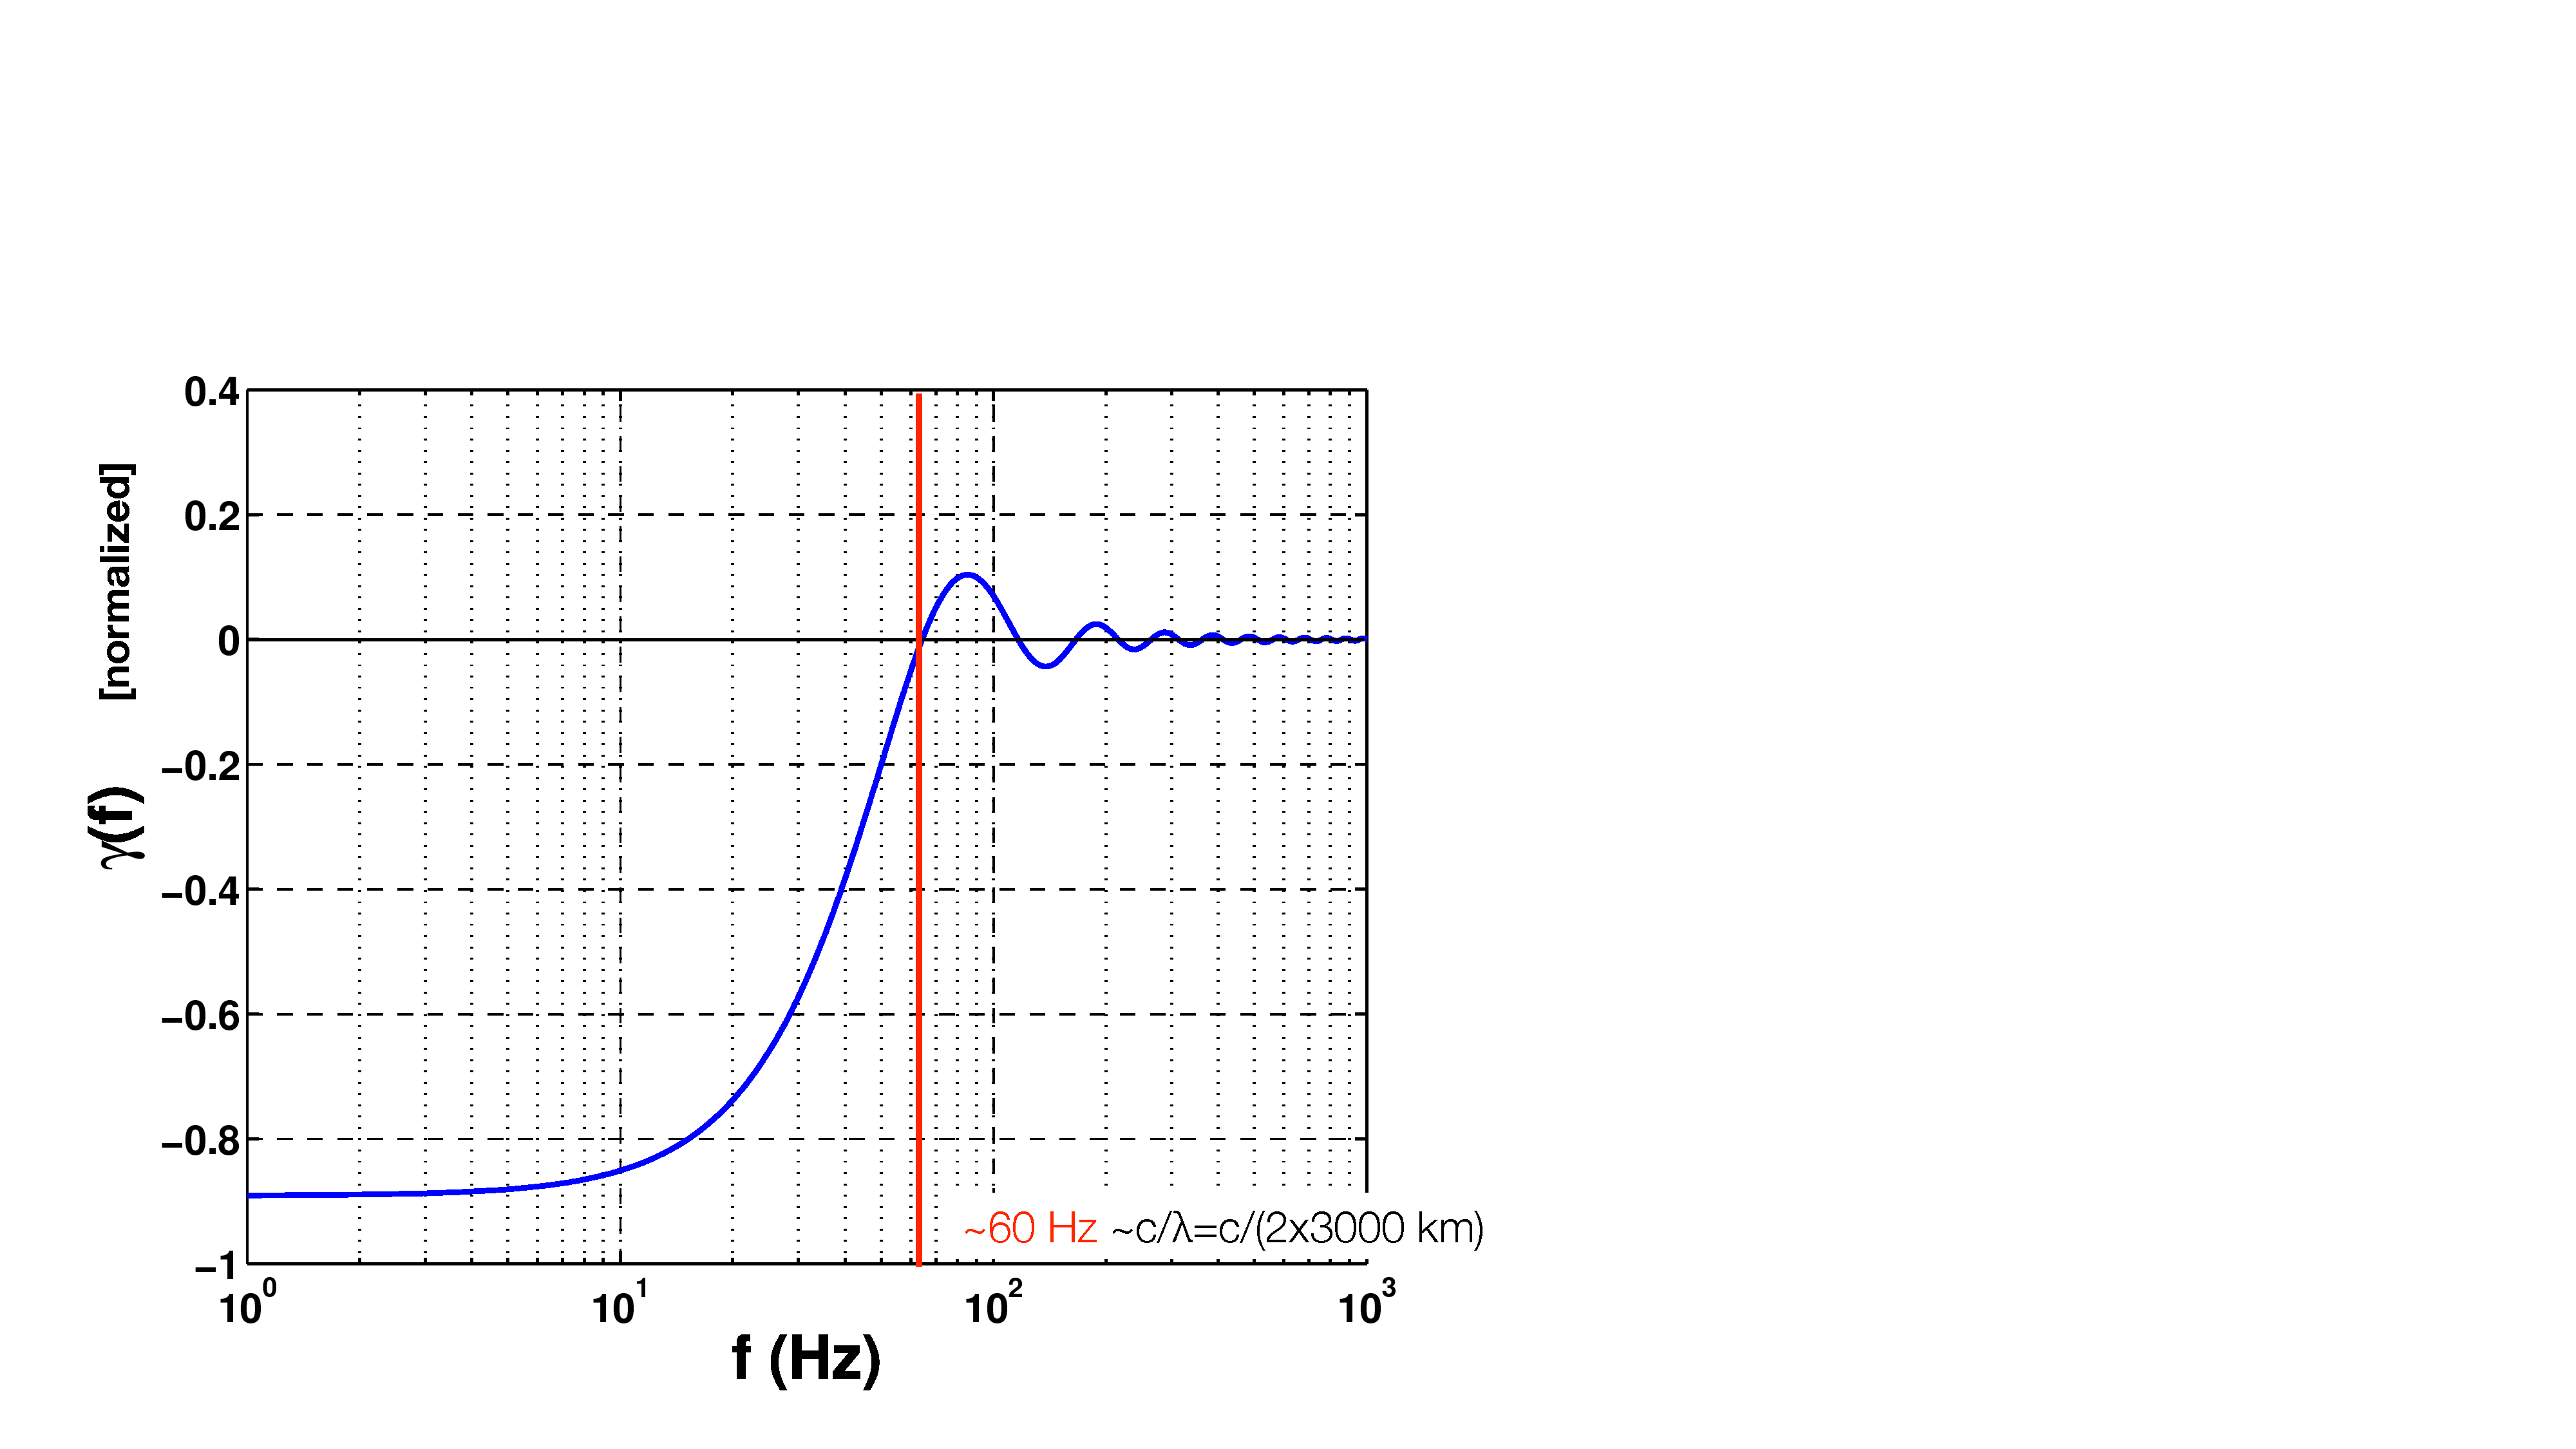
\includegraphics[width=0.49\textwidth]{Figures/LHO-LLO-orf}
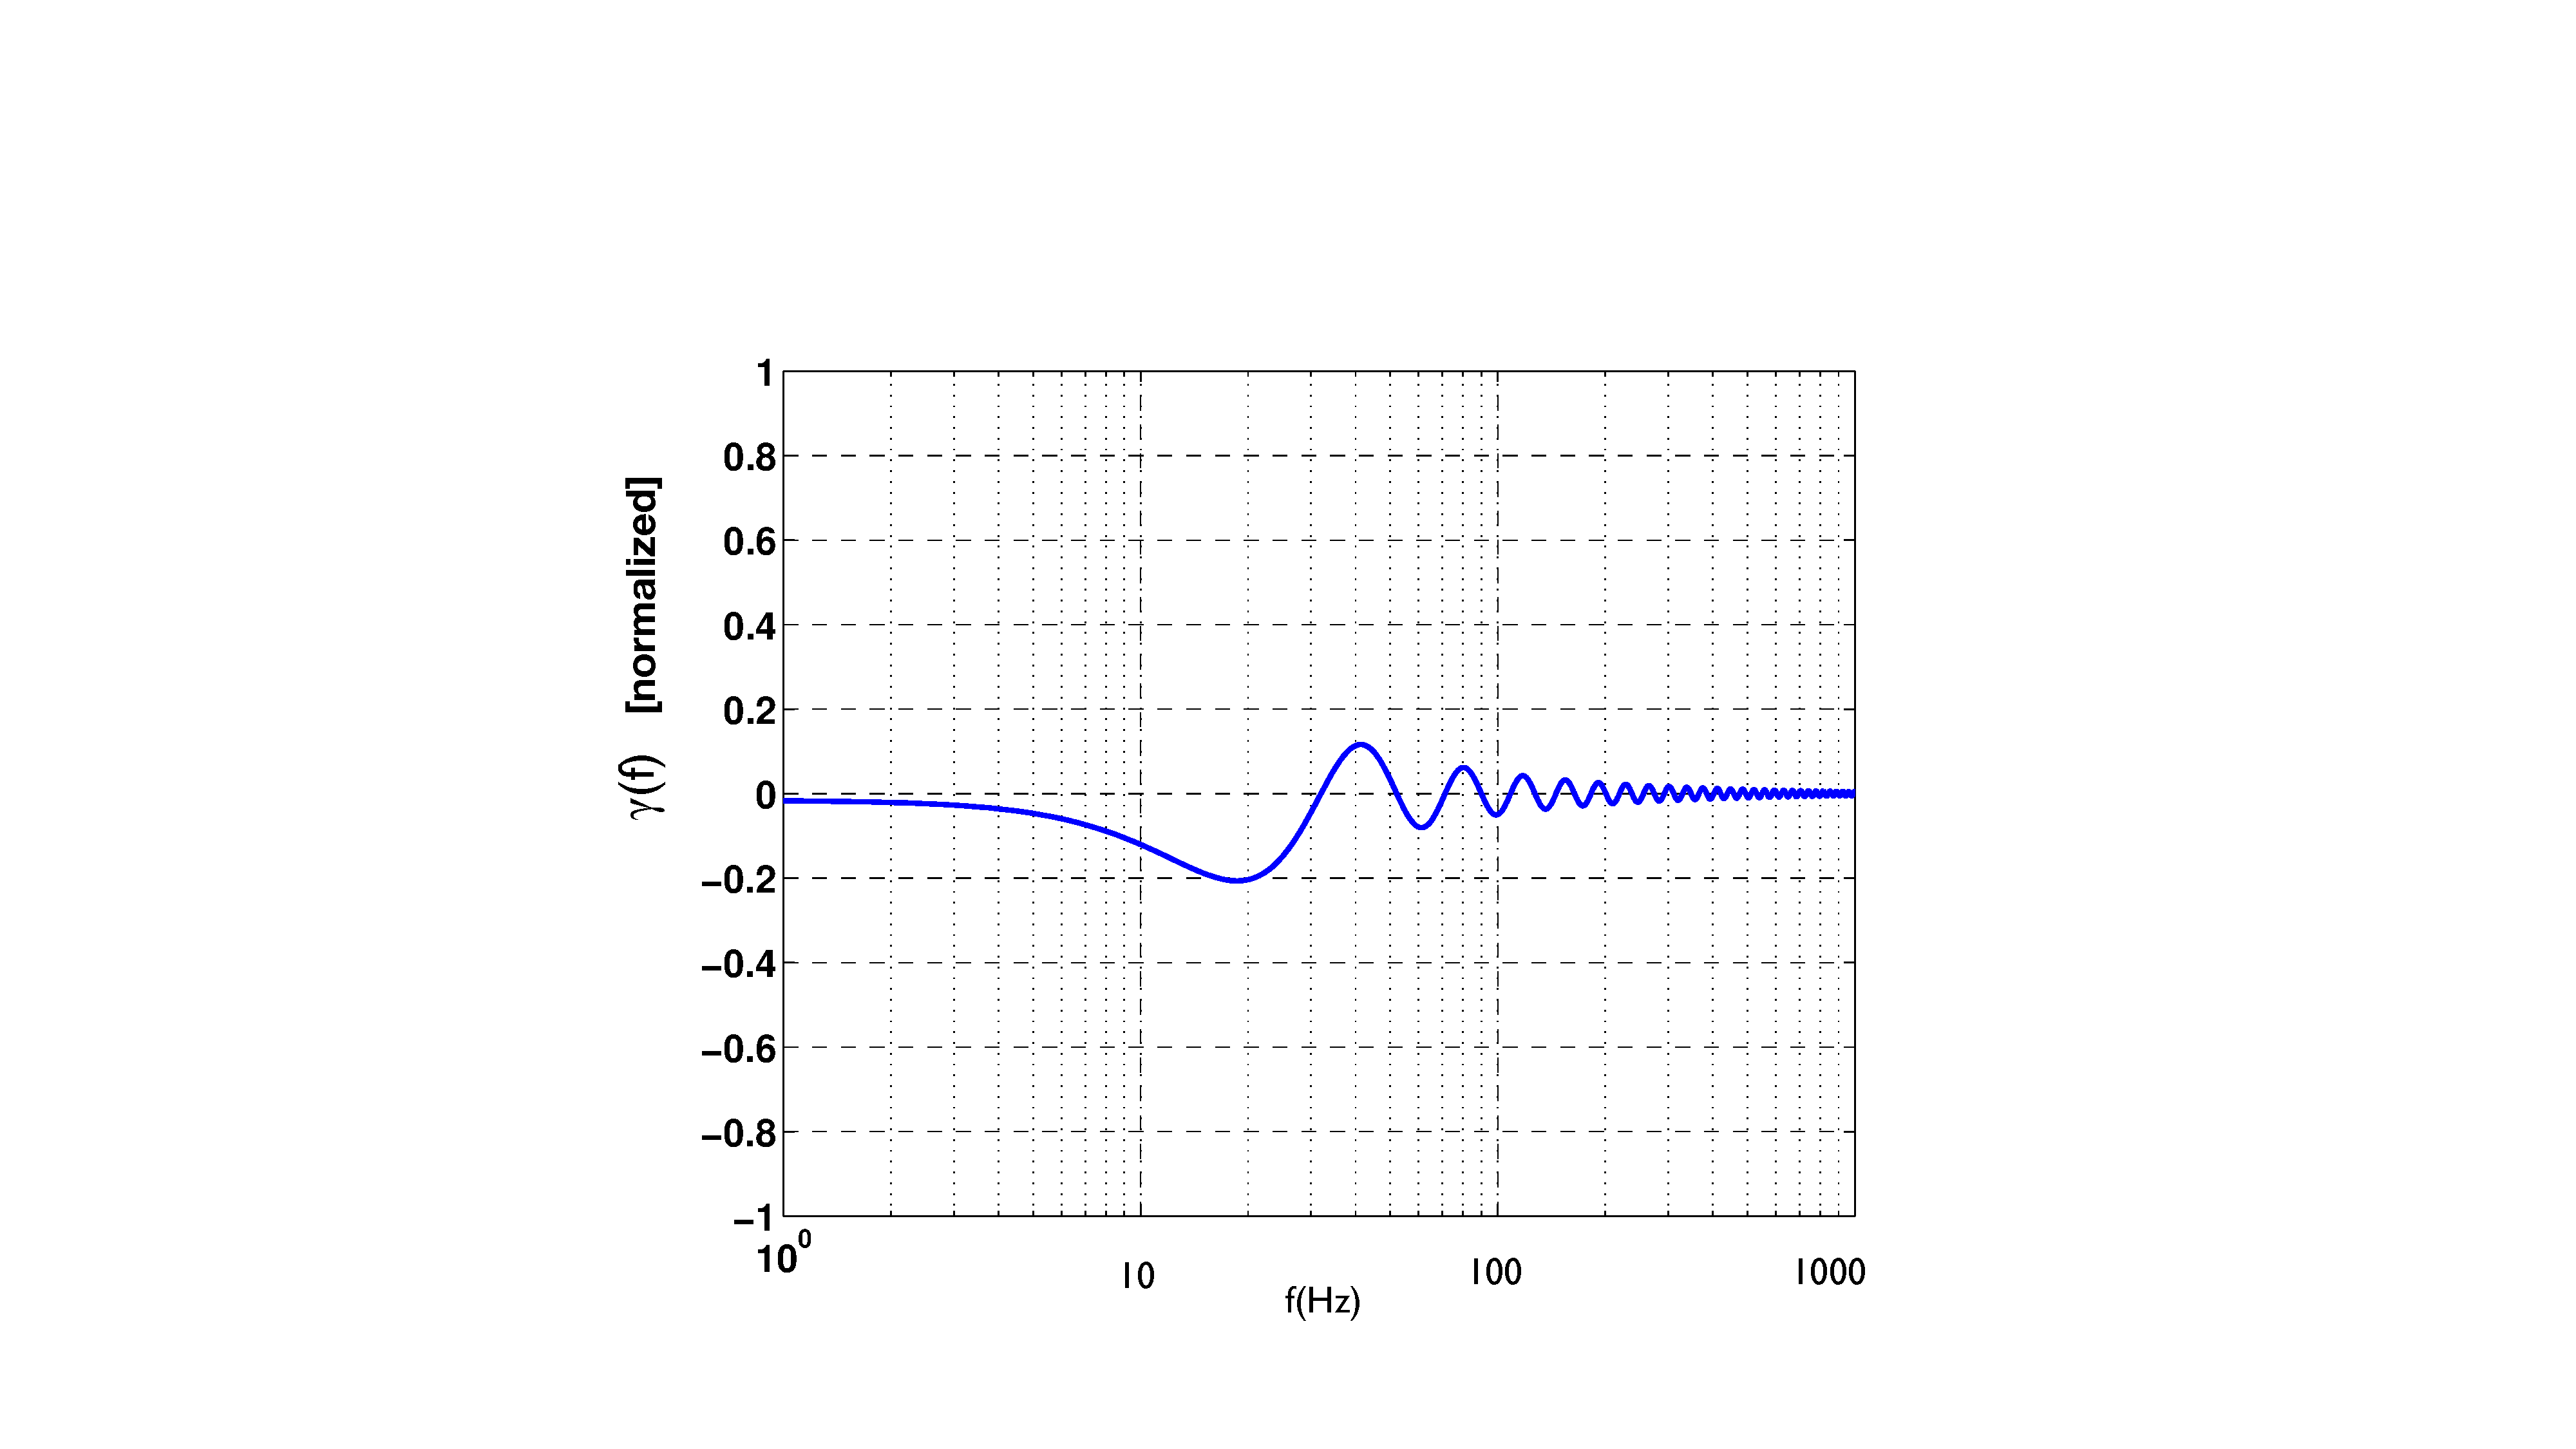
\includegraphics[width=0.49\textwidth]{Figures/LHO-Virgo-orf}
\caption{Normalized overlap function for ground-based
interferometers.
Left panel: LIGO Hanford-LIGO Livingston detector pair.
Rght panel: LIGO Hanford-Virgo detector pair.
These overlap functions were calculated in the small-antenna
approximation.
Note the reduced amplitude of the LHO-Virgo overlap function
relative to the LHO-LLO overlap function due to the much larger 
separation between Hanford, WA and Pisa, Italy.}
\label{f:orfs}
\end{center}
\end{figure}

\subsubsection{Overlap function for pulsar timing arrays}

If one uses \eqref{e:F^A(k)} for the Doppler frequency
repsonse of a pulsar timing measurement, then the correlation
between two Earth-pulsar baseline is just a single number as 
the response functions $F^A_{I,J}(\hat k)$ are independent of
frequency.
This number, which can be interpreted as the expected
correlation between the two pulsar timing measuerment, 
depends on the angular separation between the two 
Earth-pulsar baselines.
A plot of this expected correlation as a function of the 
angular separation between the Earth-pulsar baselines is
shown in Figure~\ref{f:HD_curve}.
This is called the {\em Hellings-Down curve}, originally 
calculated in 1983 by Hellings and Down~\cite{Hellings-Down:1983}.
This calculation assumes that the background is unpolarized
and isotropic.
Generalizations of the Hellings-Down curve allowing for 
anisotropy and non-general-relativity polarization modes
can be found in e.g., \cite{Mingarelli-et-al, Lee-et-al}.
The quadrupolar nature of GWs in general relativity is
apparent in the Hellings-Down curve, with an angular dependence
that is qualitatively similar to $\cos(2\zeta)$, where 
$\zeta$ is the angle between two Earth-pulsar baselines.
%
\begin{figure}[htbp!]
\begin{center}
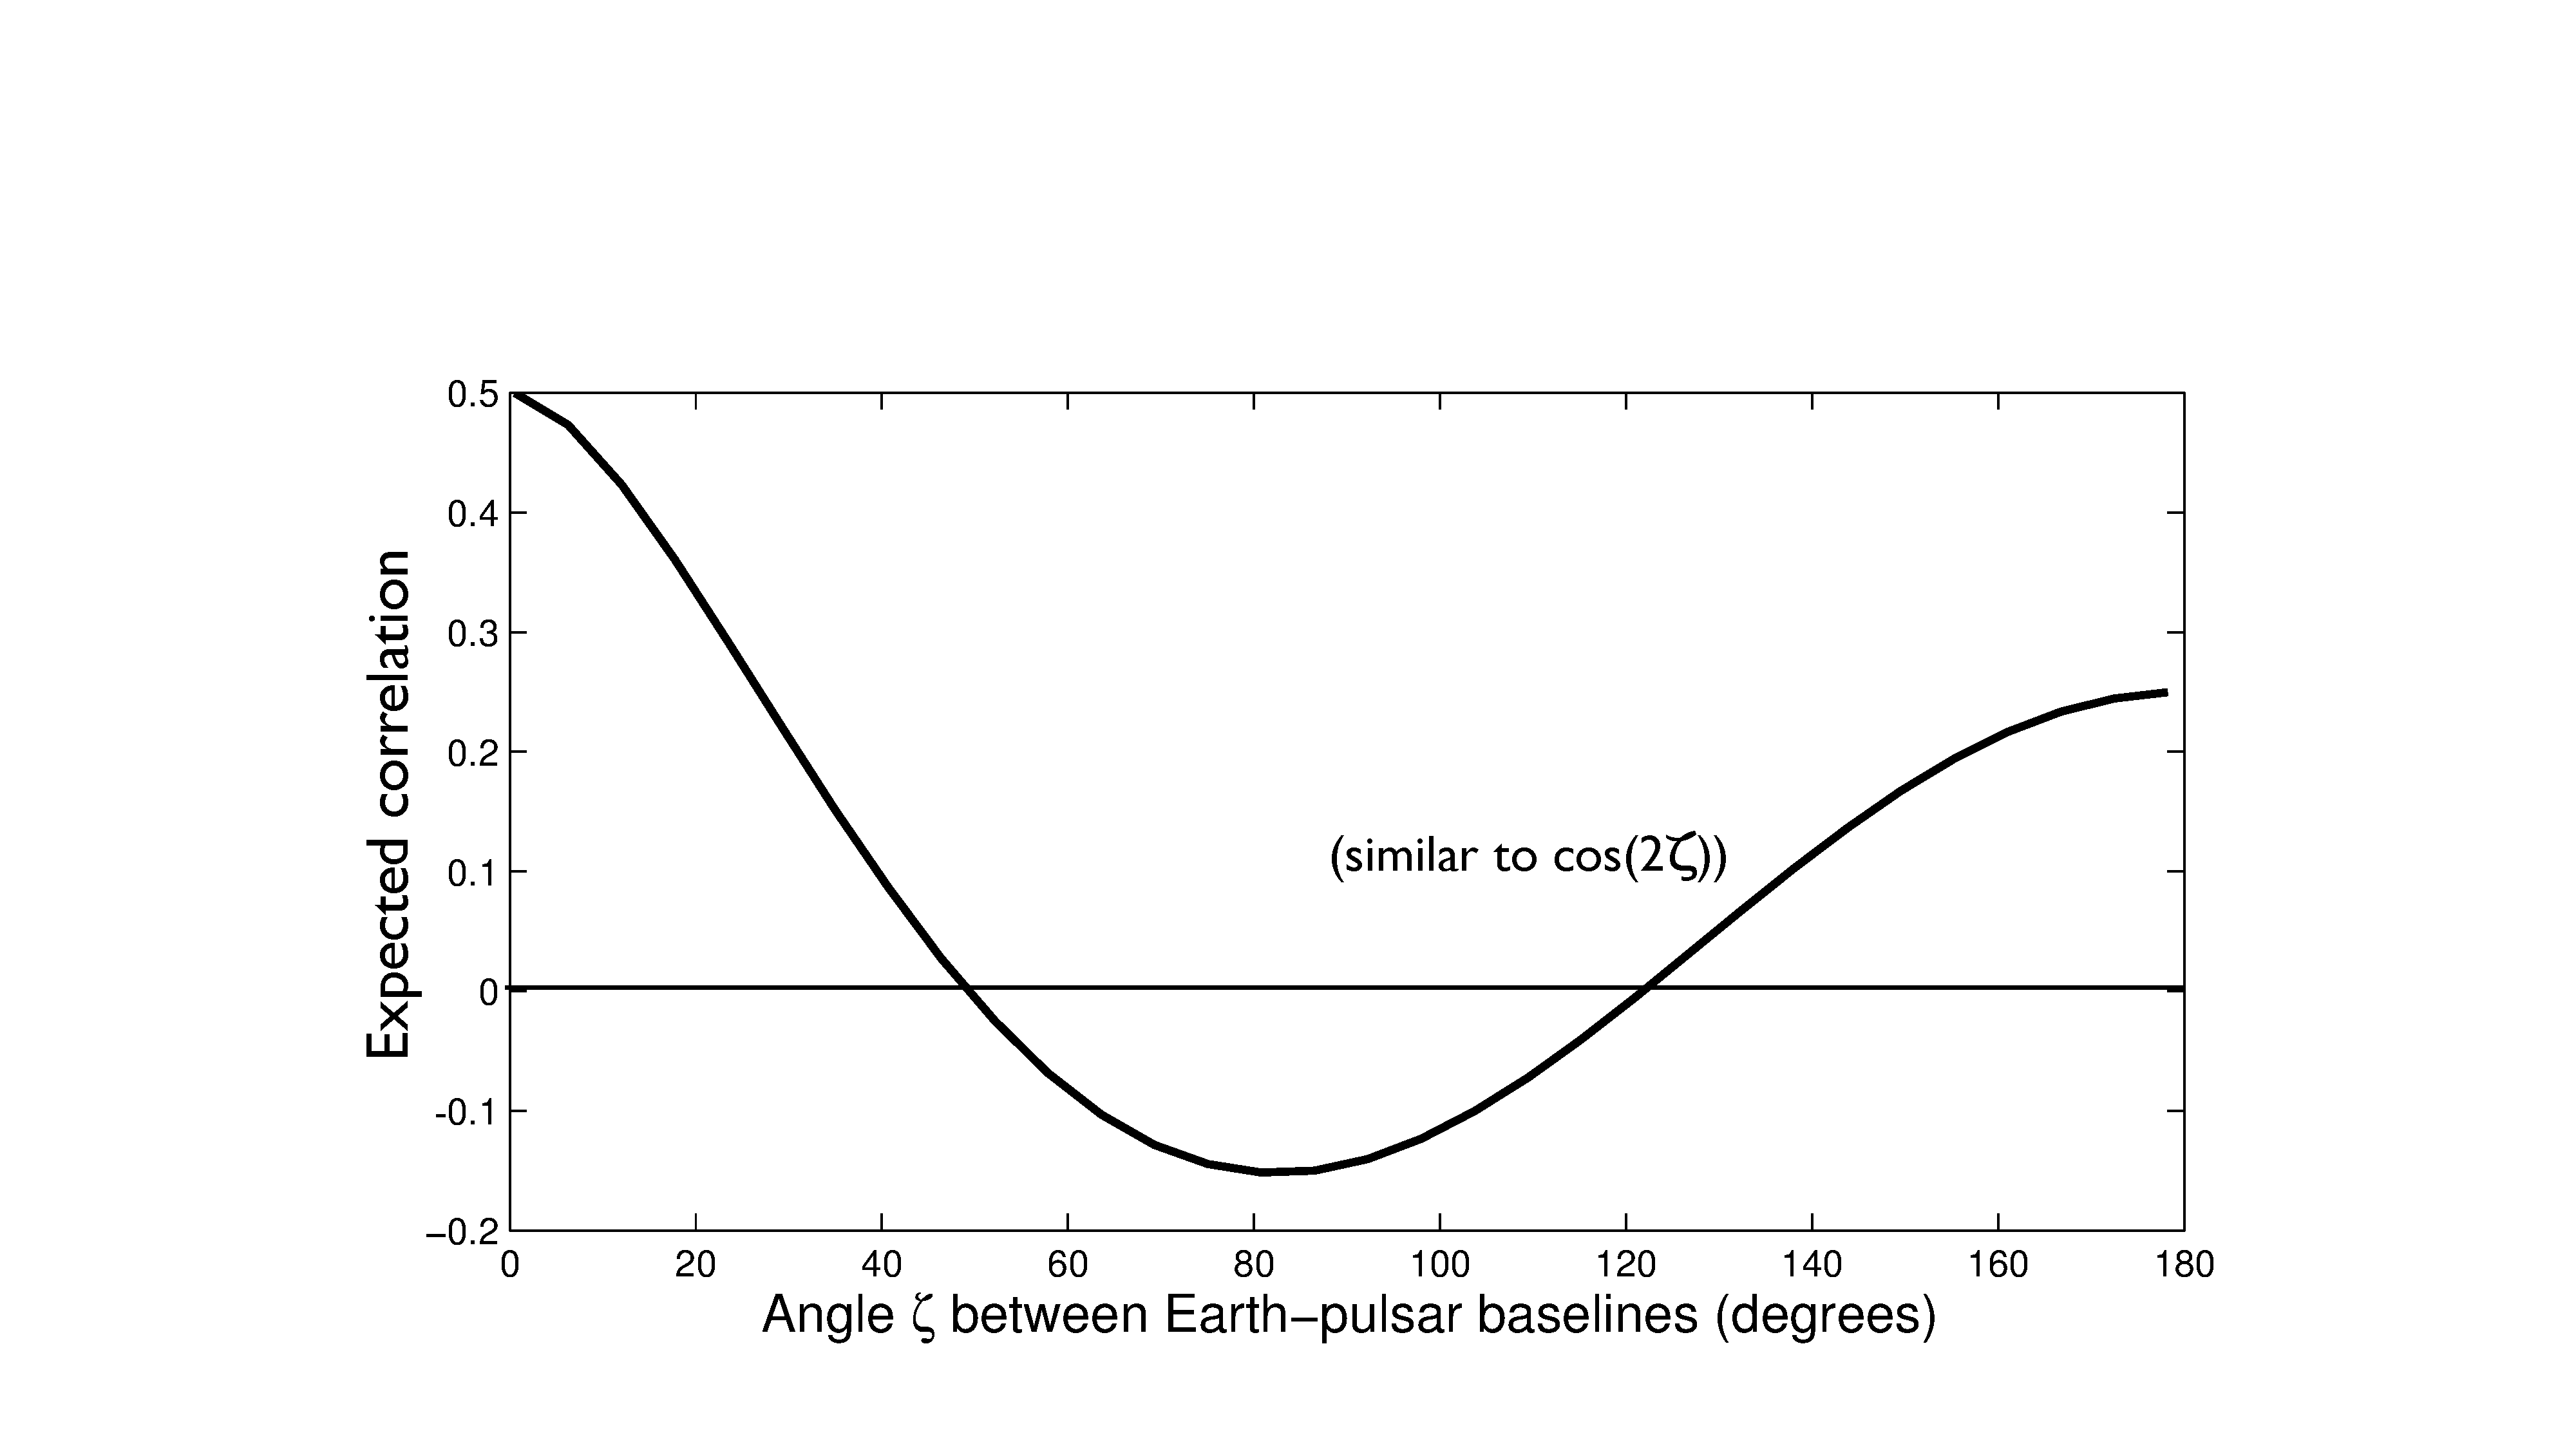
\includegraphics[width=0.7\textwidth]{Figures/HD_curve}
\caption{Hellings-Down curve.
The values of the expected correlation for an unpolarized,
isotropic GWB as a function of the angle $\zeta$ between
two Earth-pulsar baselines.}
\label{f:HD_curve}
\end{center}
\end{figure}

\subsubsection{Overlap function for a pair of electric dipole 
antennas}

For the final example, you are asked in Exercise 7 to 
calculate the 

\begin{figure}[htbp!]
\begin{center}
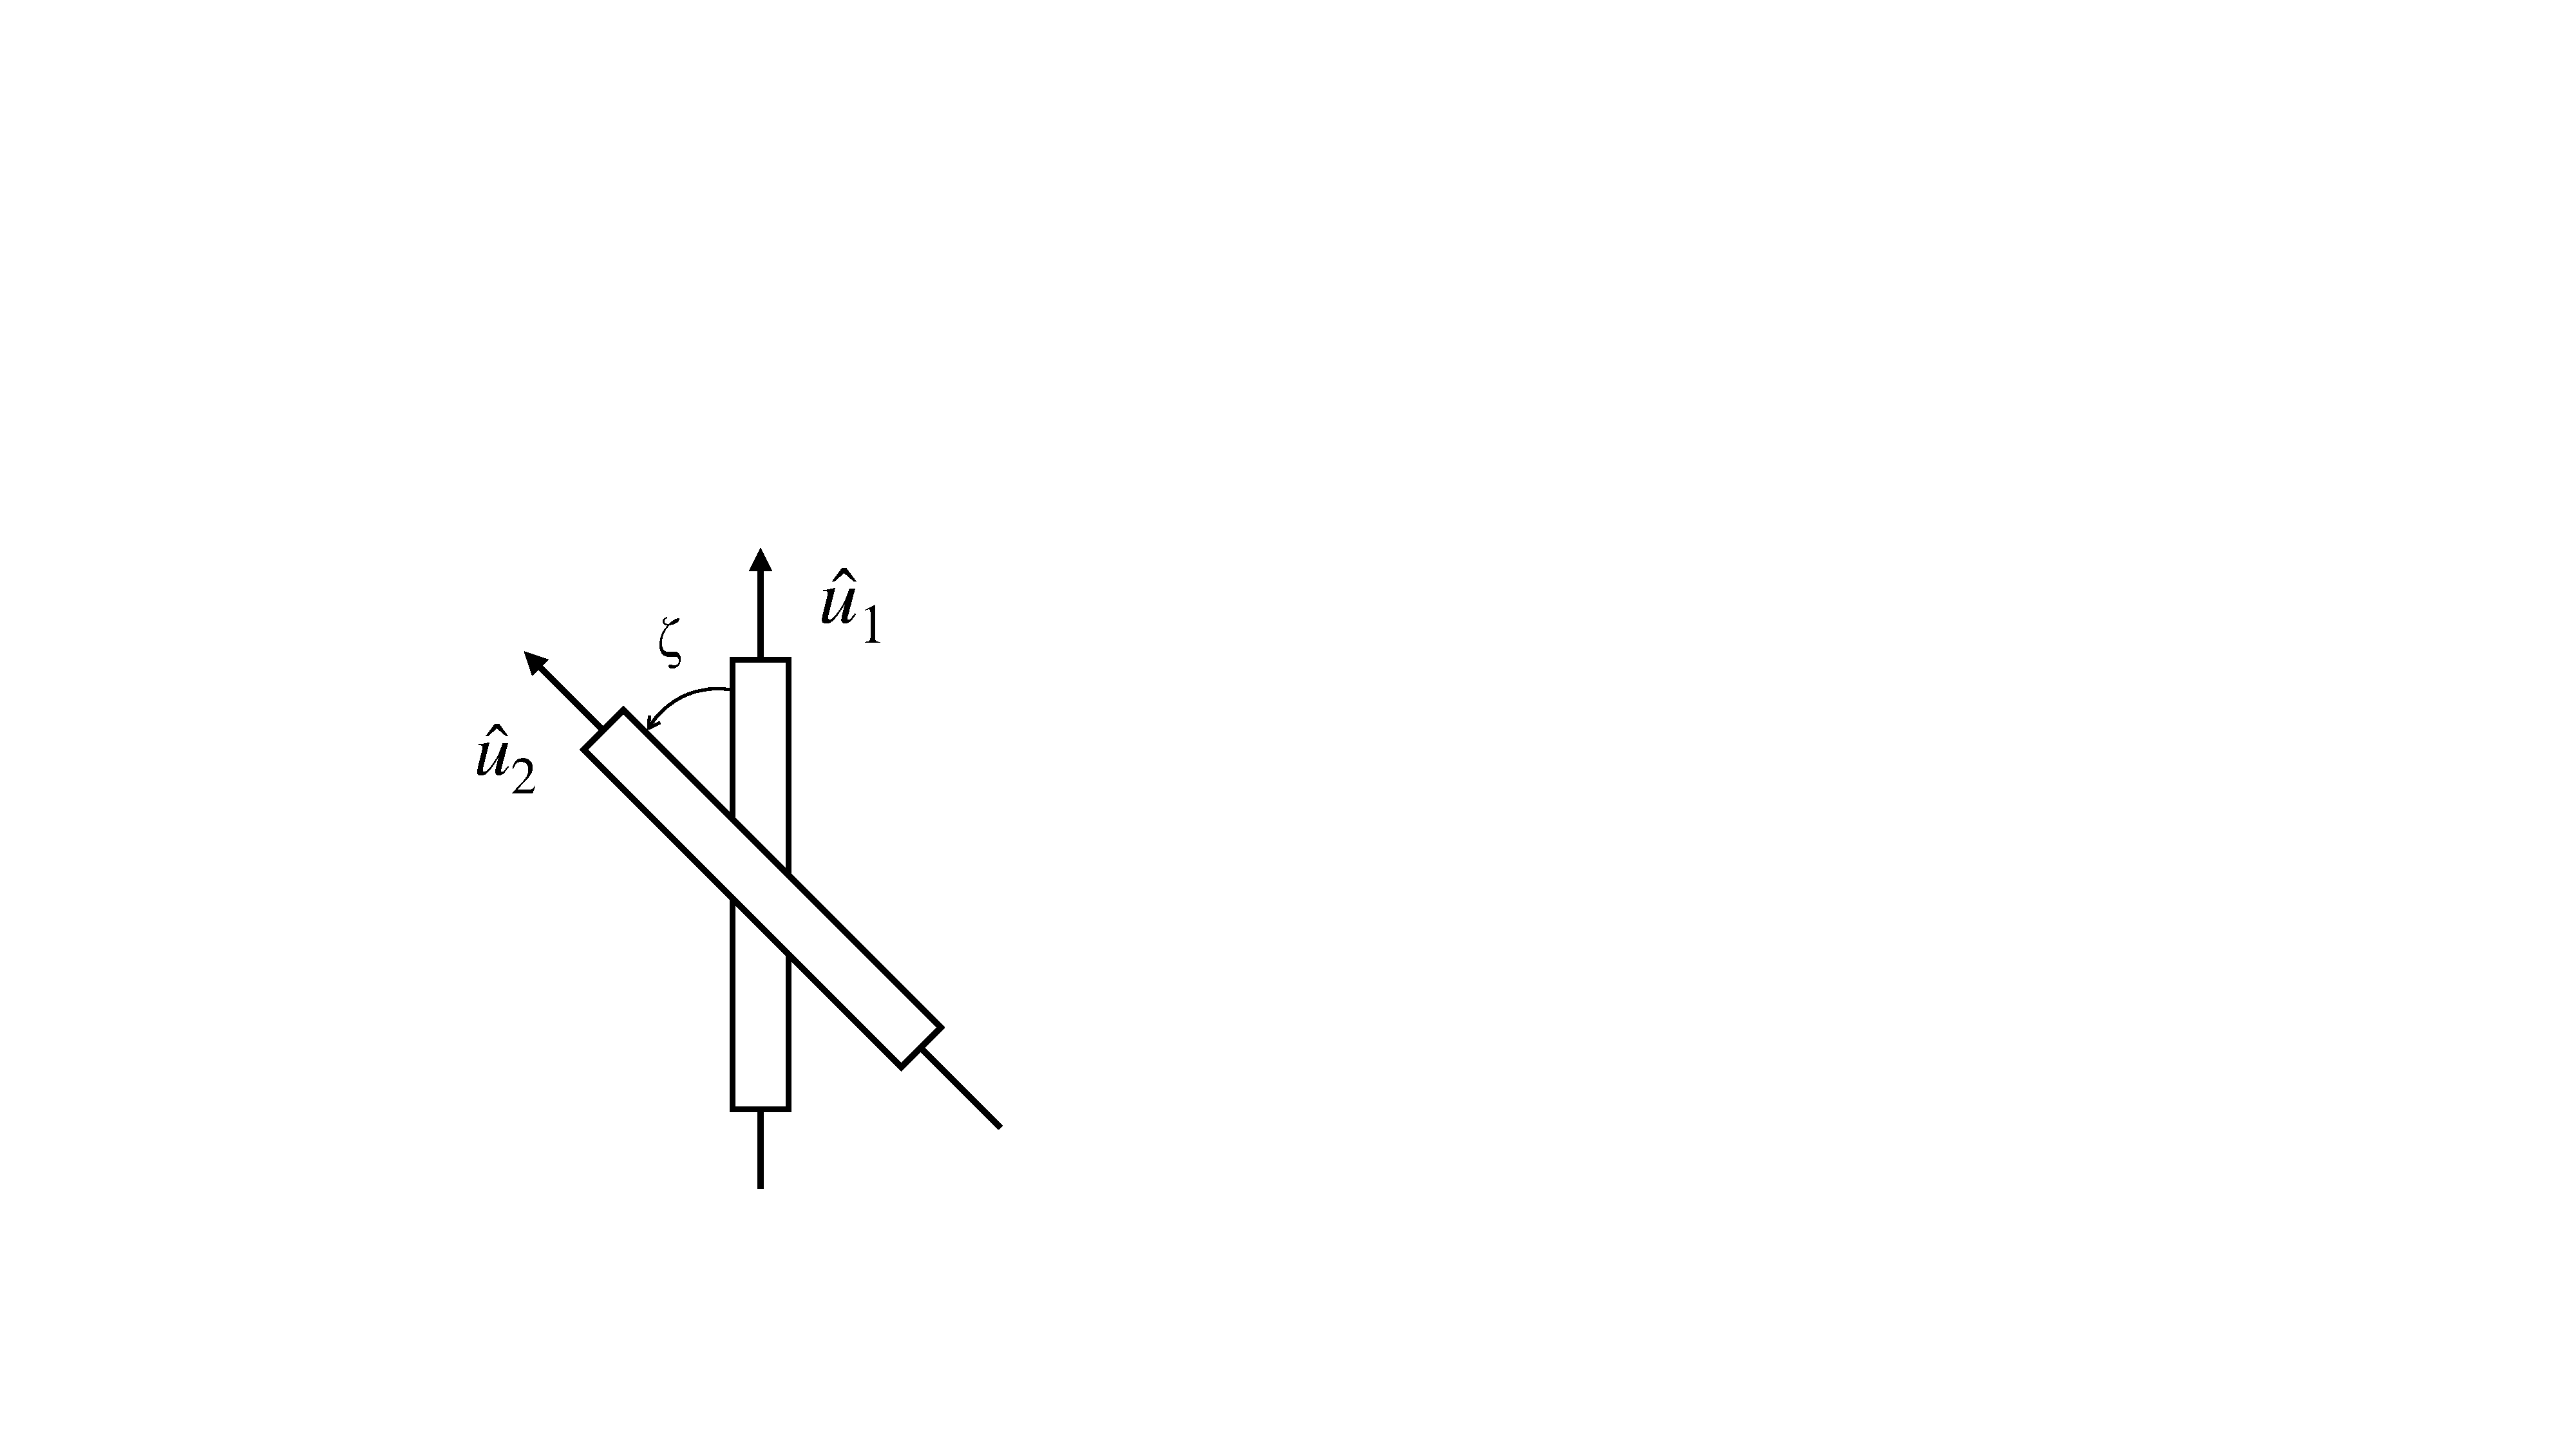
\includegraphics[width=0.25\textwidth]{Figures/dipole-orf}
\caption{Geometry for calculating the overlap function
for a pair of short, electric dipole antennae, for an
unpolarized and isotropic electric field
(Exercise 7).}
\label{f:dipole-orf}
\end{center}
\end{figure}

%%%%%%%%%%%%%%%%%%%%%%%%%%%%%%%%%%%%%%%%%%%%%%%%%%%%%%%
\section{What to do in the absence of correlations?}

\begin{figure}[htbp!]
\begin{center}
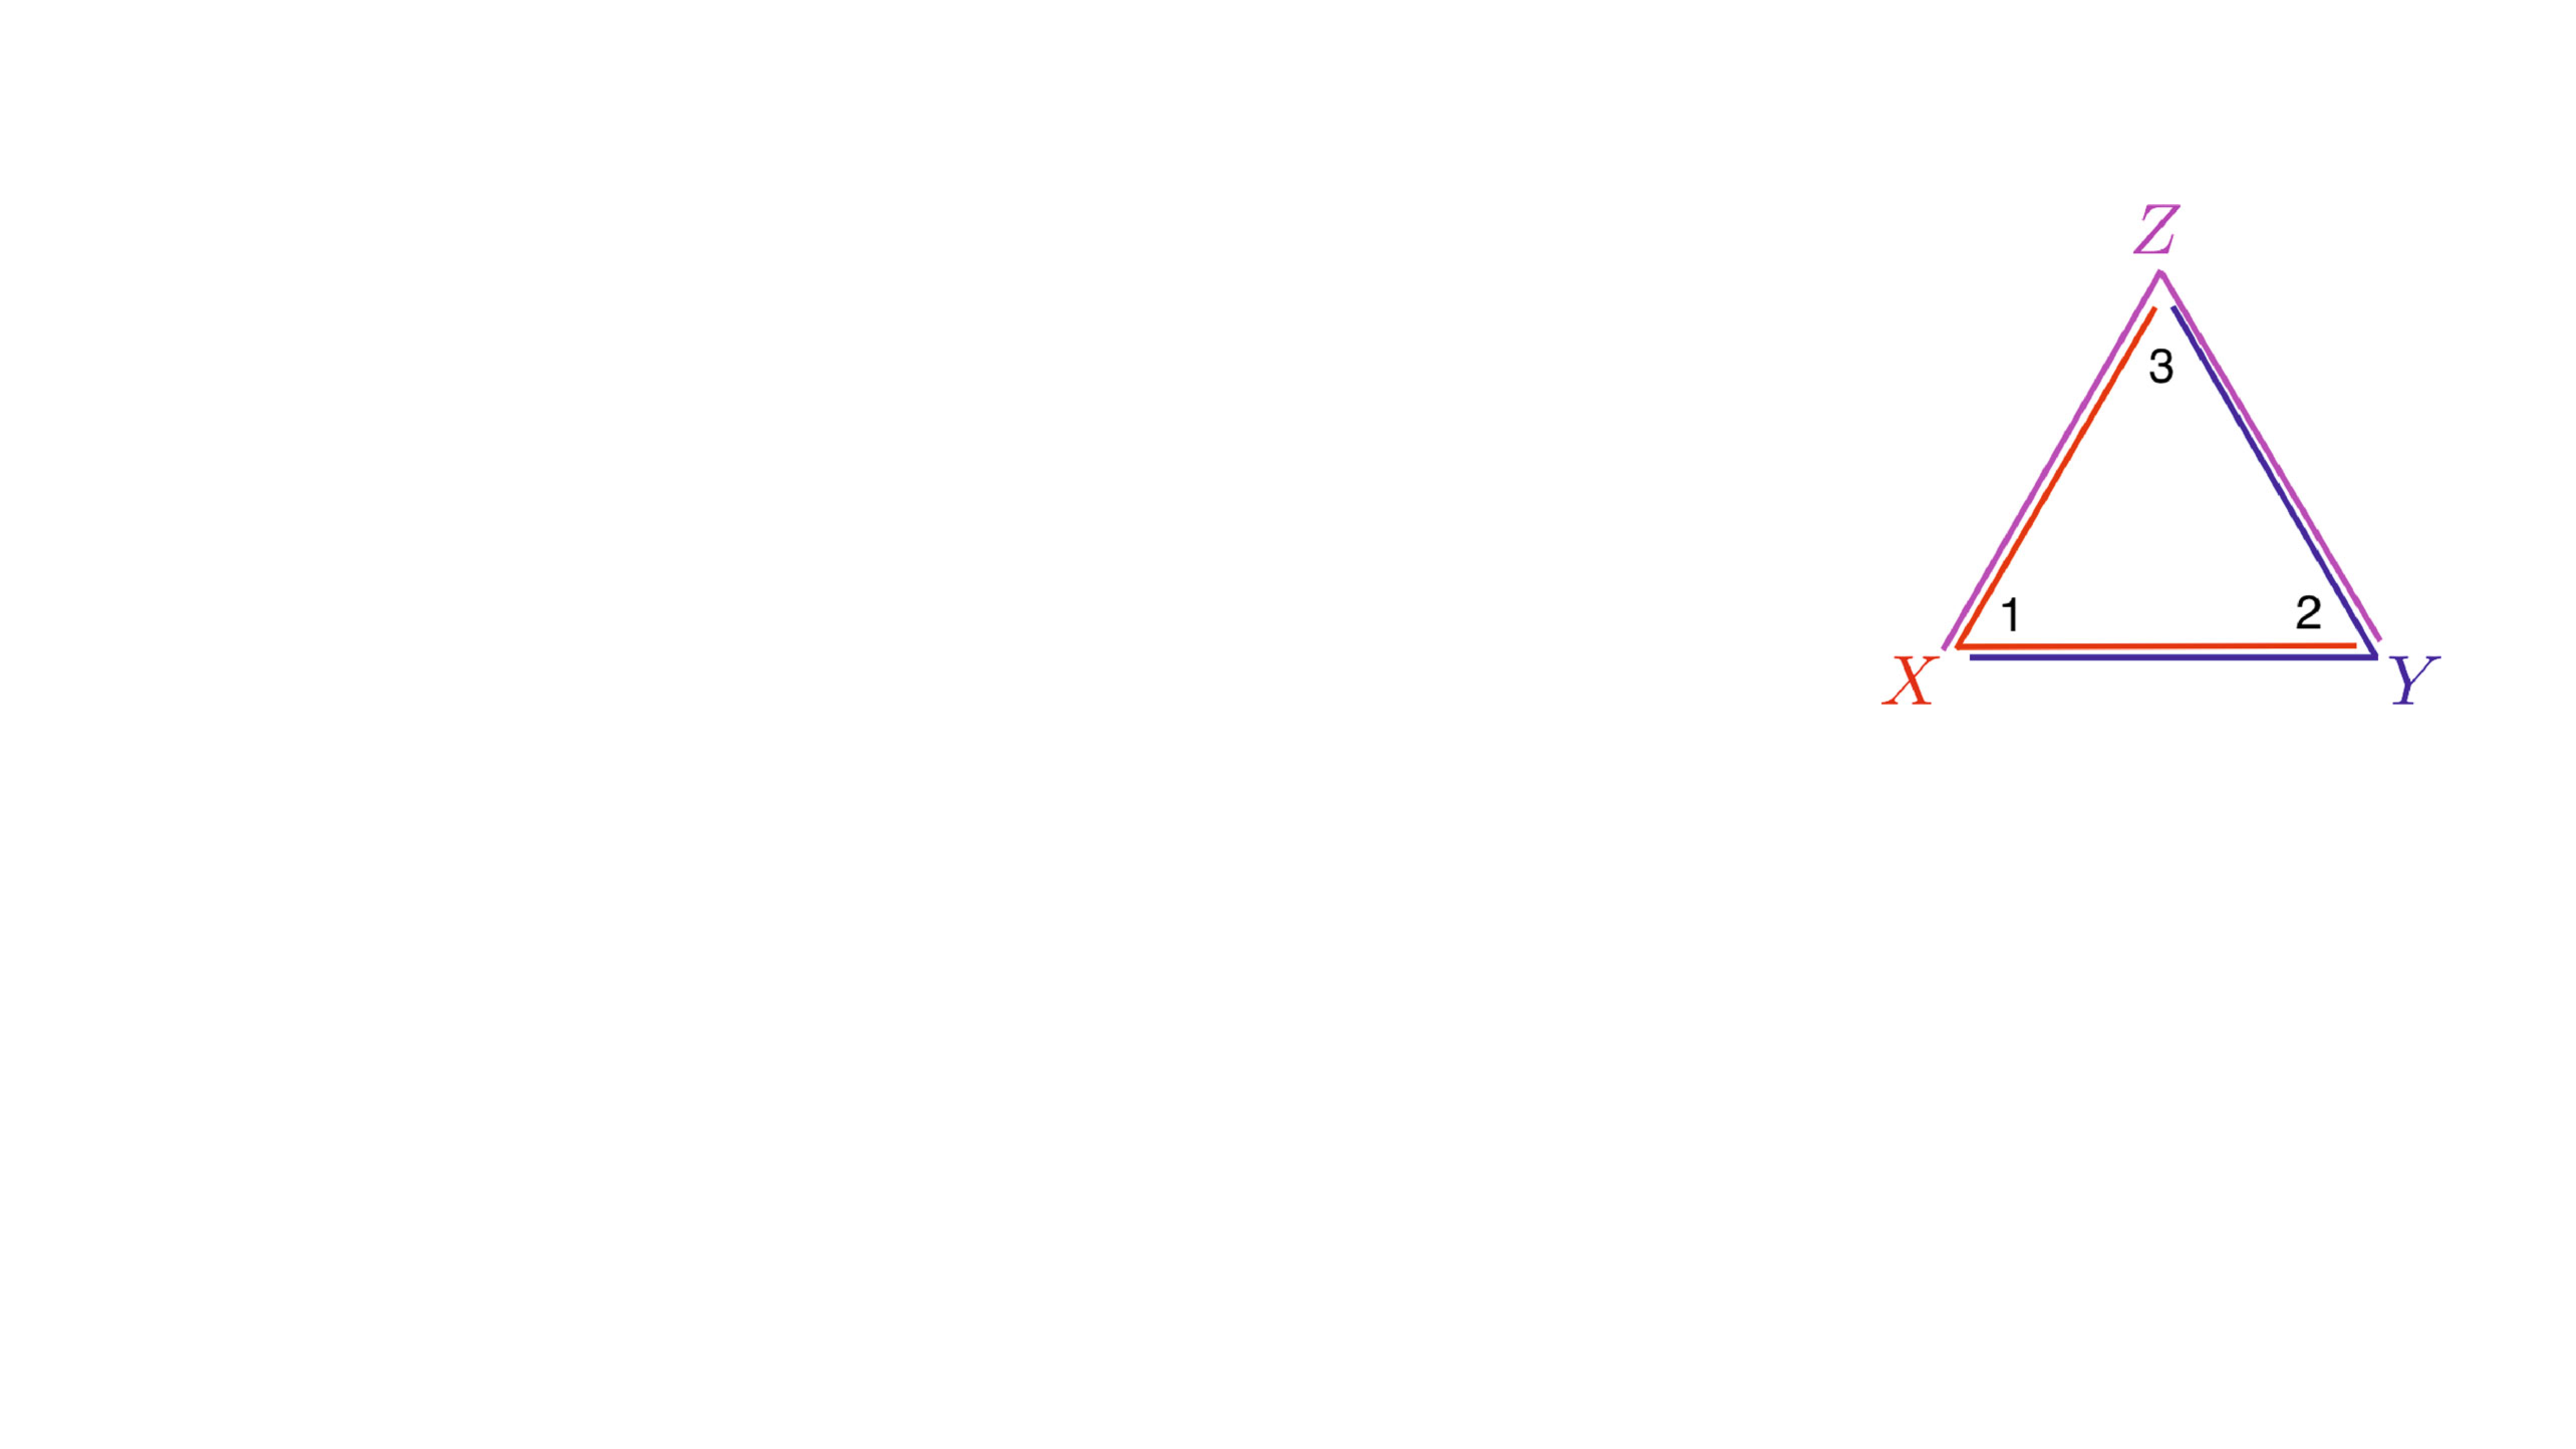
\includegraphics[width=0.3\textwidth]{Figures/LISA_XYZ}
\caption{Schematic representation of the LISA consellation.
$X$, $Y$, $Z$ correspond to Michelson interferometers 
with $60^\circ$ opening angles between the arms, with vertices
located at spacecraft 1, 2, 3.
From $X, Y, Z$, one can construct the TDI combinations
$A, E, T$ described in the text.}
\label{f:LISA_XYZ}
\end{center}
\end{figure}

\begin{figure}[htbp!]
\begin{center}
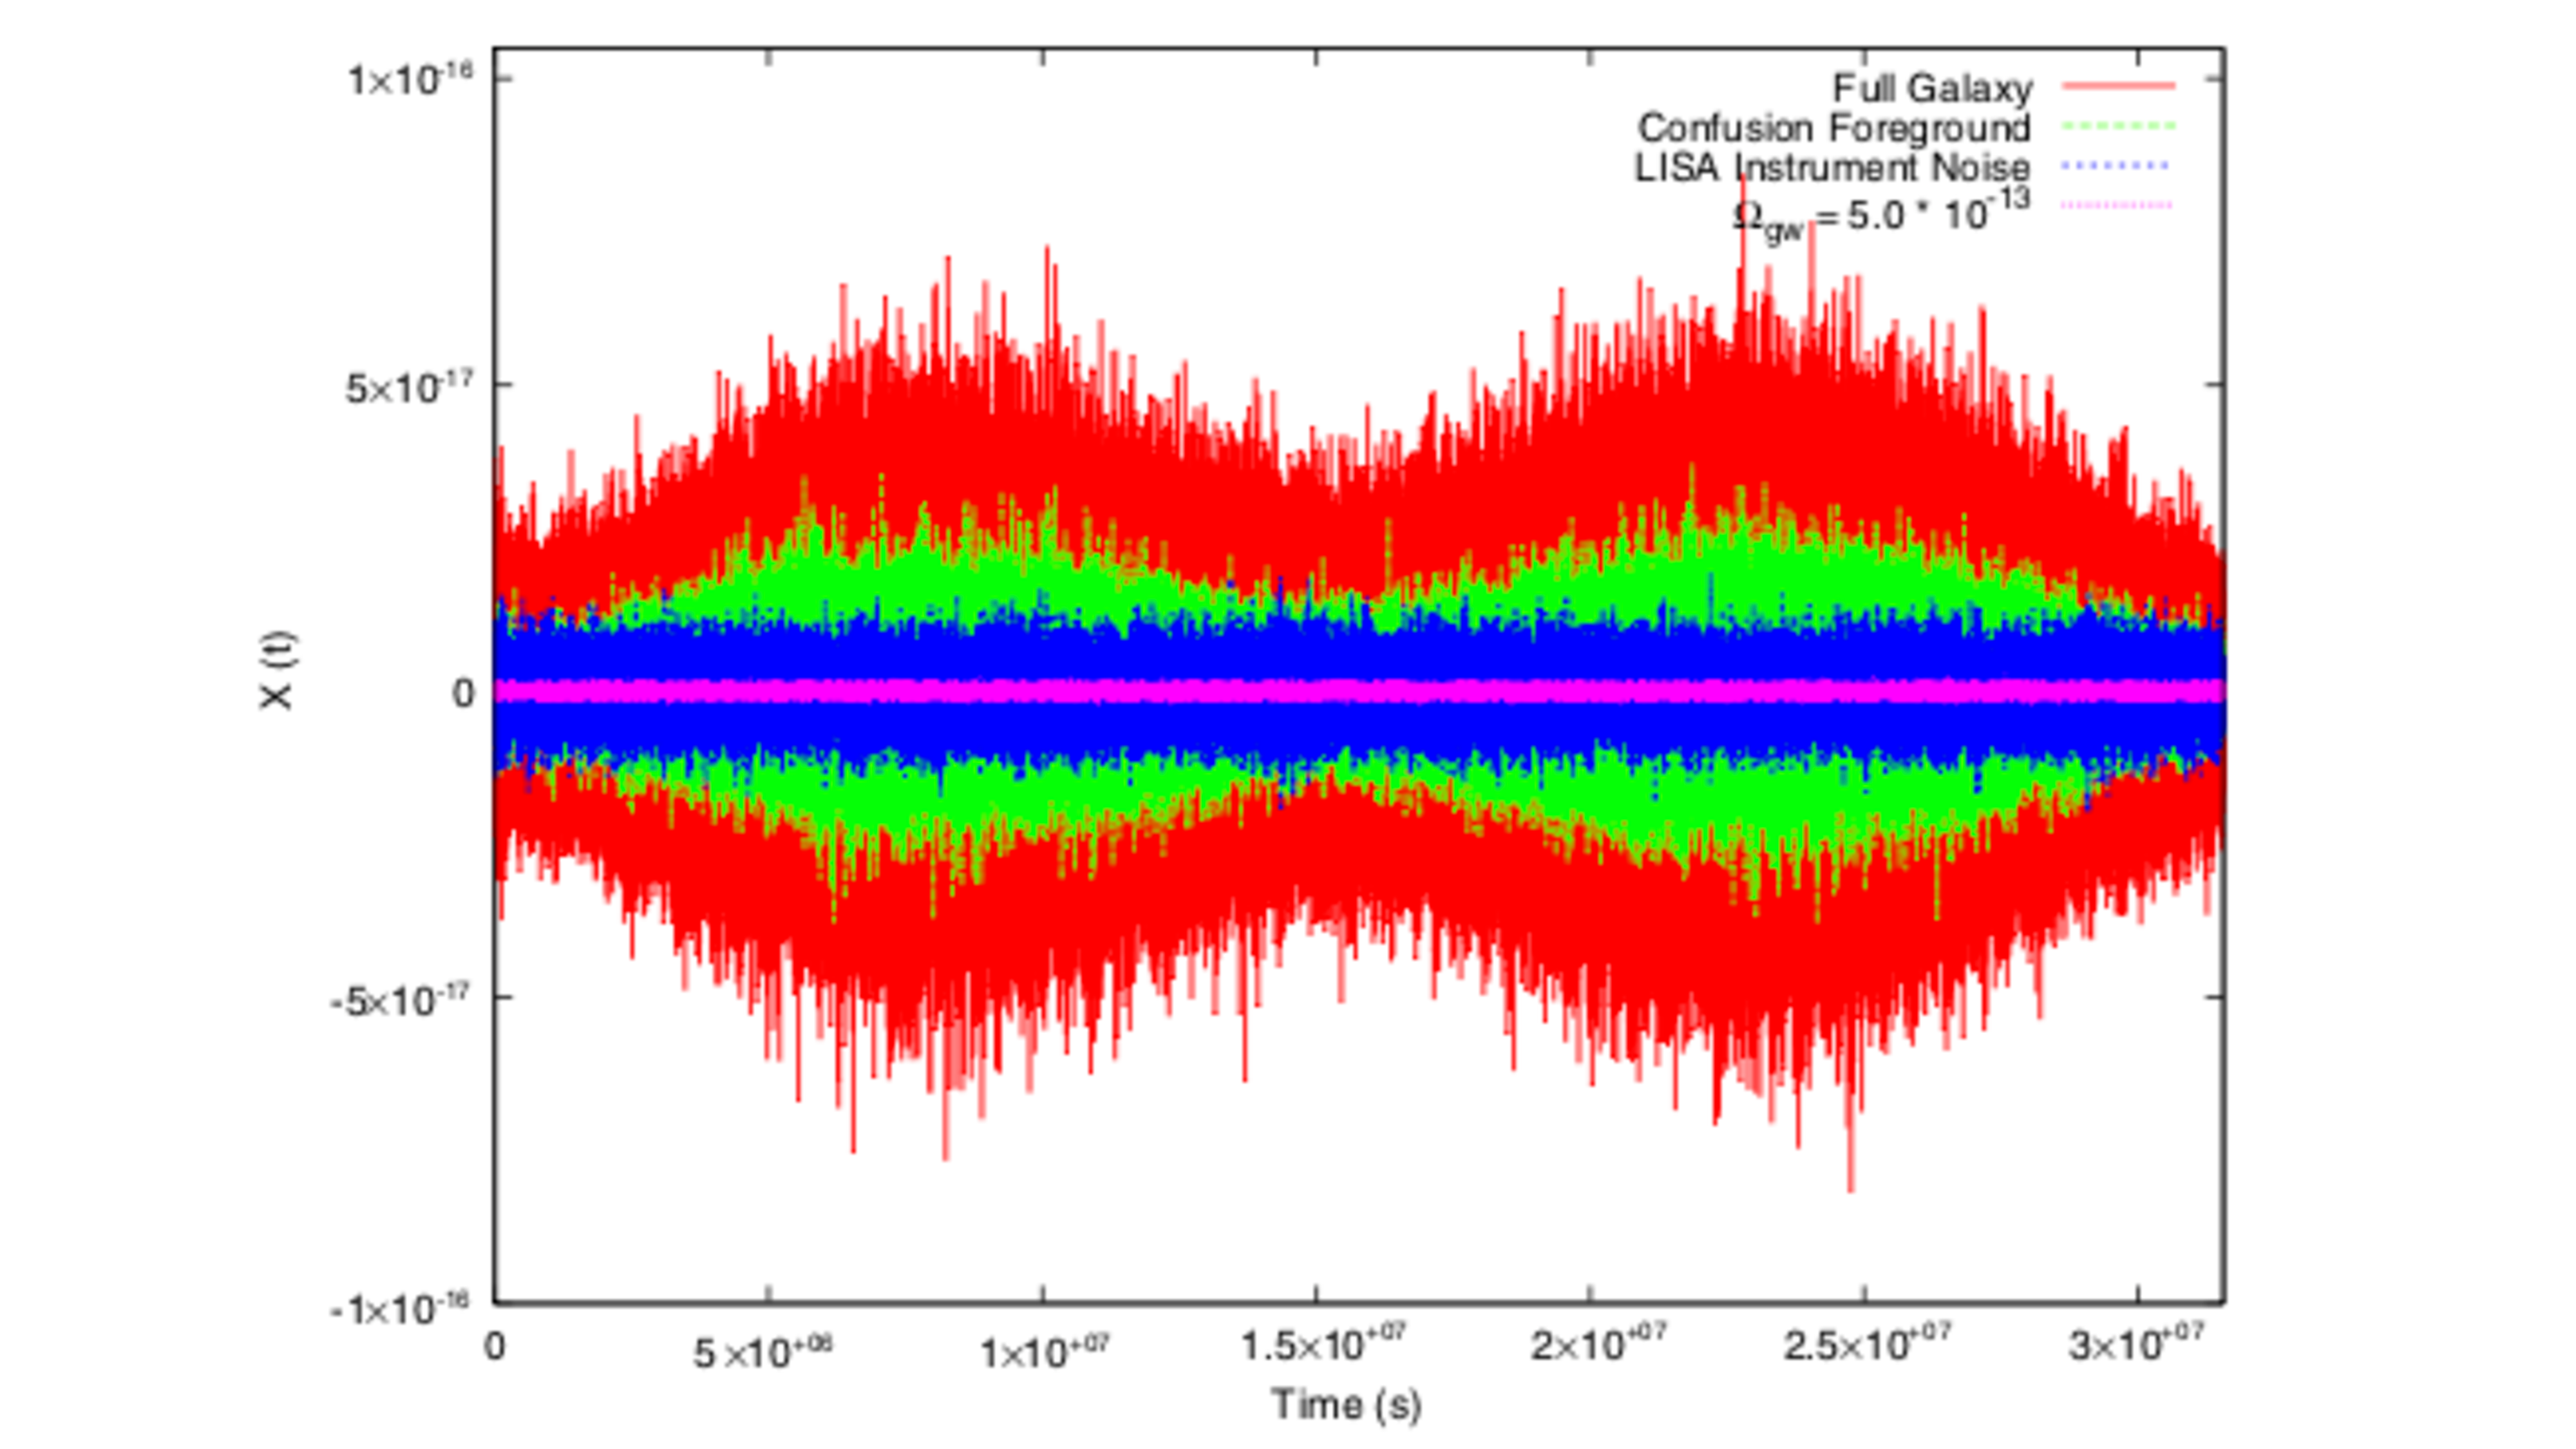
\includegraphics[width=0.7\textwidth]{Figures/LISA_timeseries}
\caption{One-years worth of simulated timeseries data for LISA.
The total output consists of a cosmological GWB (pink);
LISA instrument noise (blue); the full astrophysical foreground
signal from the galactic white-dwarf binary population (red),
which consist of individually resolvable binary signal and 
the confusion-limited foreground (green).
Of particular note are the amplitude and time variability 
of the astrophysical foreground, having a period of 6~months.
Figure taken from \cite{Adams-Cornish:2014}.}
\label{f:LISA_timeseries}
\end{center}
\end{figure}
\begin{figure}[htbp!]

\begin{center}
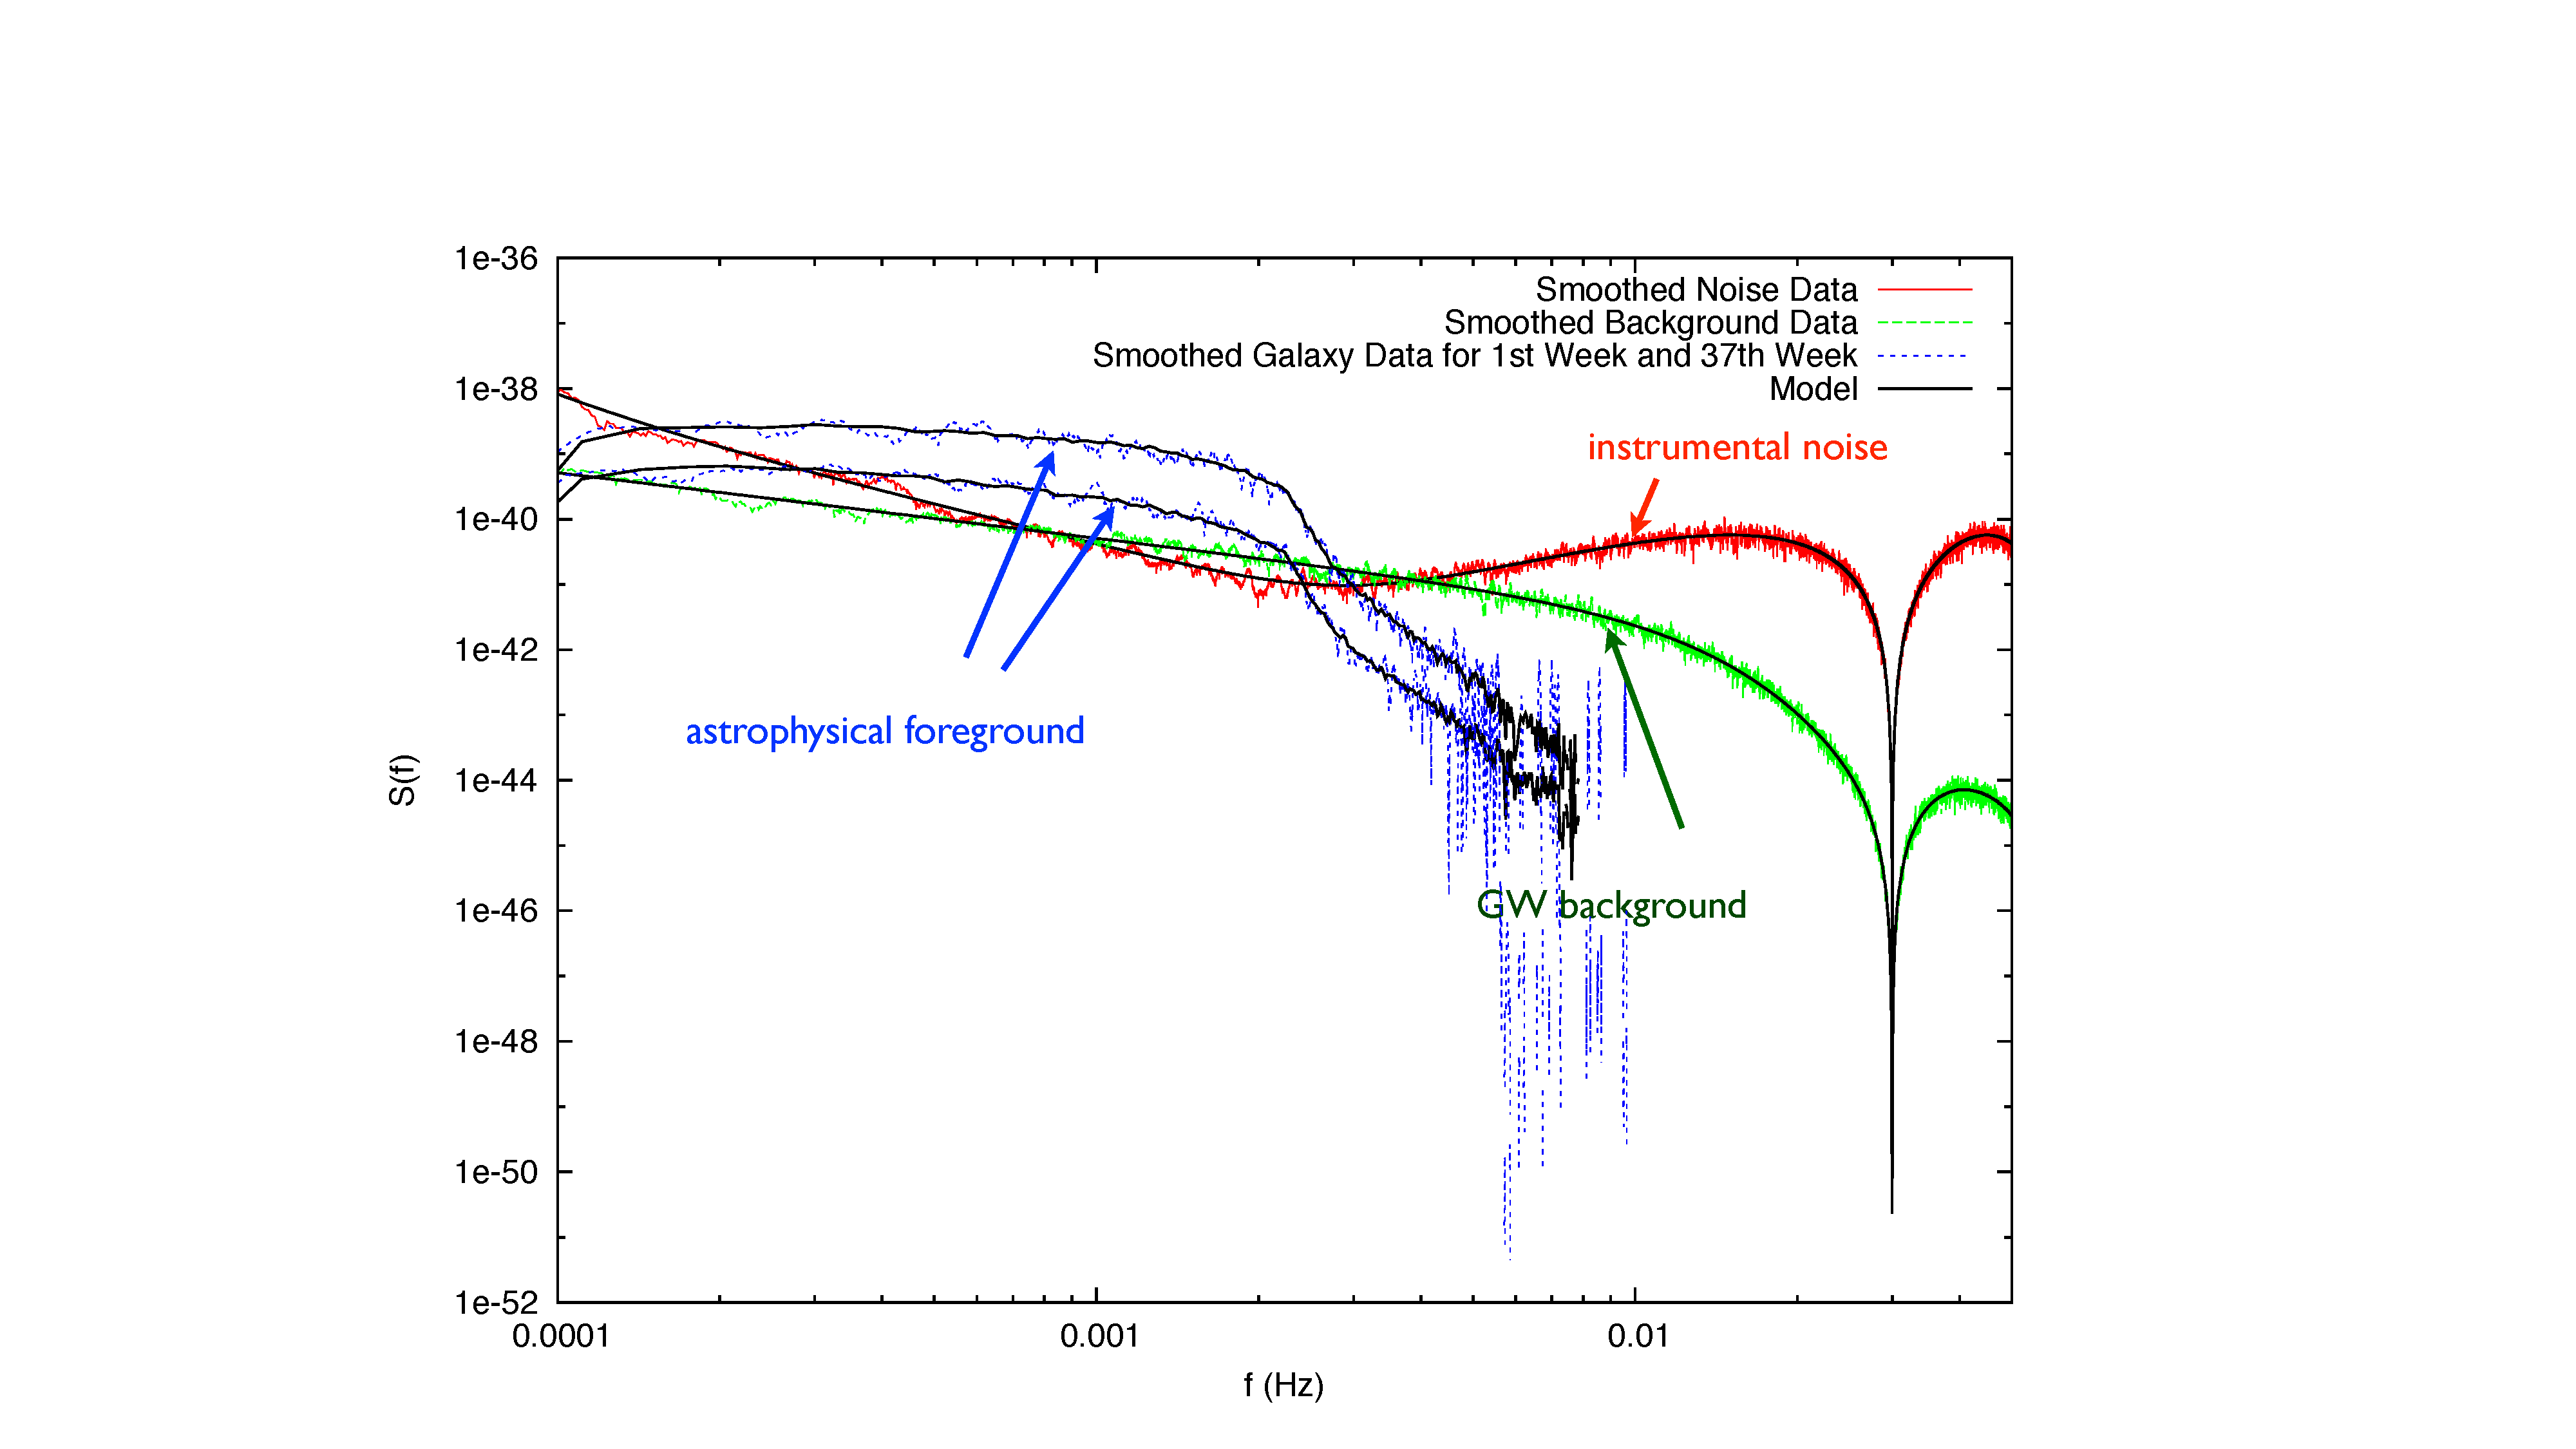
\includegraphics[width=0.6\textwidth]{Figures/LISA_psds}
\caption{Simulated power spectral densities for the 
LISA instrumental noise (red), cosmological GWB (green)
and astrophysical foreground from galactic white dwarf
binaries (blue), the latter at two times during LISAs orbit.
Note the strength of the astrophyical foreground relative
to the instrumental noise, and the different spectral shapes
for the three different contributions.
Figure taken from \cite{Adams-Cornish:2014}.}
\label{f:LISA_psds}
\end{center}
\end{figure}

%%%%%%%%%%%%%%%%%%%%%%%%%%%%%%%%%%%%%%%%%%%%%%%%%%%%%%%
\section{Frequentist statistics and Bayesian inference}

Bayes' theorem:
%
\be
p(H|d) = \frac{p(d|H) p(H)}{p(d)}
\ee

Posterior distributions:
\be
p(S_{n_1}, S_{n_2}, S_h|d,{\cal M}_1) 
= \frac{p(d|S_{n_1}, S_{n_2}, S_h, {\cal M}_1)p(S_{n_1}, S_{n_2}, S_h|{\cal M}_1)}{p(d|{\cal M}_1)}
\ee

\be
p(S_h|d,{\cal M}_1) 
= \int {\rm d}S_{n_1}\>\int{\rm d}S_{n_2}\>p(S_{n_1}, S_{n_2}, S_h|d,{\cal M}_1)
\ee

Model selection:
\be
\frac{p({\cal M}_1|d)}{p({\cal M}_0|d)} =
\frac{p(d|{\cal M}_1)\,p({\cal M}_1)}
{p(d|{\cal M}_0)\,p({\cal M}_0)}
\ee

Relationship between Bayesian and frequentist approaches:
\be
{\cal B}_{10}(d) 
\equiv\frac{p(d|{\cal M}_1)}{p(d|{\cal M}_0)}
= \frac{
\int{\rm d}\vec\theta_n
\int{\rm d}\vec\theta_h
\>p(d|\vec\theta_n,\vec\theta_h,{\cal M}_1)p(\vec\theta_n,\vec\theta_h|{\cal M}_1)}
{\int {\rm d}\vec\theta_n\>p(d|\vec\theta_n,{\cal M}_0)p(\vec\theta_n|{\cal M}_0)}
\simeq\Lambda_{\rm ML}(d)\,\frac{\Delta V_1/V_1}{\Delta V_0/V_0}
\ee

\be
\ee

\be
\ee

\be
\ee

\be
\ee

\be
\ee

\be
\ee

\be
\ee

\be
\ee

\be
\ee

\be
\ee

\be
\ee

\be
\ee

\be
\ee

\be
\ee

\be
\ee

\be
\ee



\begin{table}[tb]
\addtocounter{table}{-1}
\centering
\begin{longtable}{p{2.75in} | p{2.75in}}
\hline
FREQUENTIST STATISTICS & BAYESIAN INFERENCE\\
\hline
probabilities are long-run relative occurrence of 
outcomes of repeatable experiments (i.e., random variables);
cannot be assigned to hypotheses or parameters, 
which have fixed but unknown values
&
probabilities are degree of belief (or confidence)
in any proposition, and hence 
can be assigned to hypotheses and parameters
\\
\hline
usually start with a likelihood function $p(d|H)$,
which is the probability distribution for the 
measured data $d$, assuming the truth of a particular
hypothesis $H$
&
same as frequentist approach
\\
\hline
construct statistics for parameter estimation and
hypothesis testing
&
specify prior degree of belief for parameters and 
hypotheses
\\
\hline
calculate the probability distribution of the 
statistic (e.g., using time slides)
&
use Bayes' theorem to update degree of belief in
light of new data 
\\
\hline
construct confidence intervals and $p$-values
&
construct posteriors and odds ratios (Bayes factors)
\\
\hline
\end{longtable}
\vspace{0.2 in}
\caption{Comparison of frequentist and Bayesian approaches
to statistical inference.}
\label{t:bayesfreq}
\end{table}

\begin{figure}[htbp!]
\begin{center}
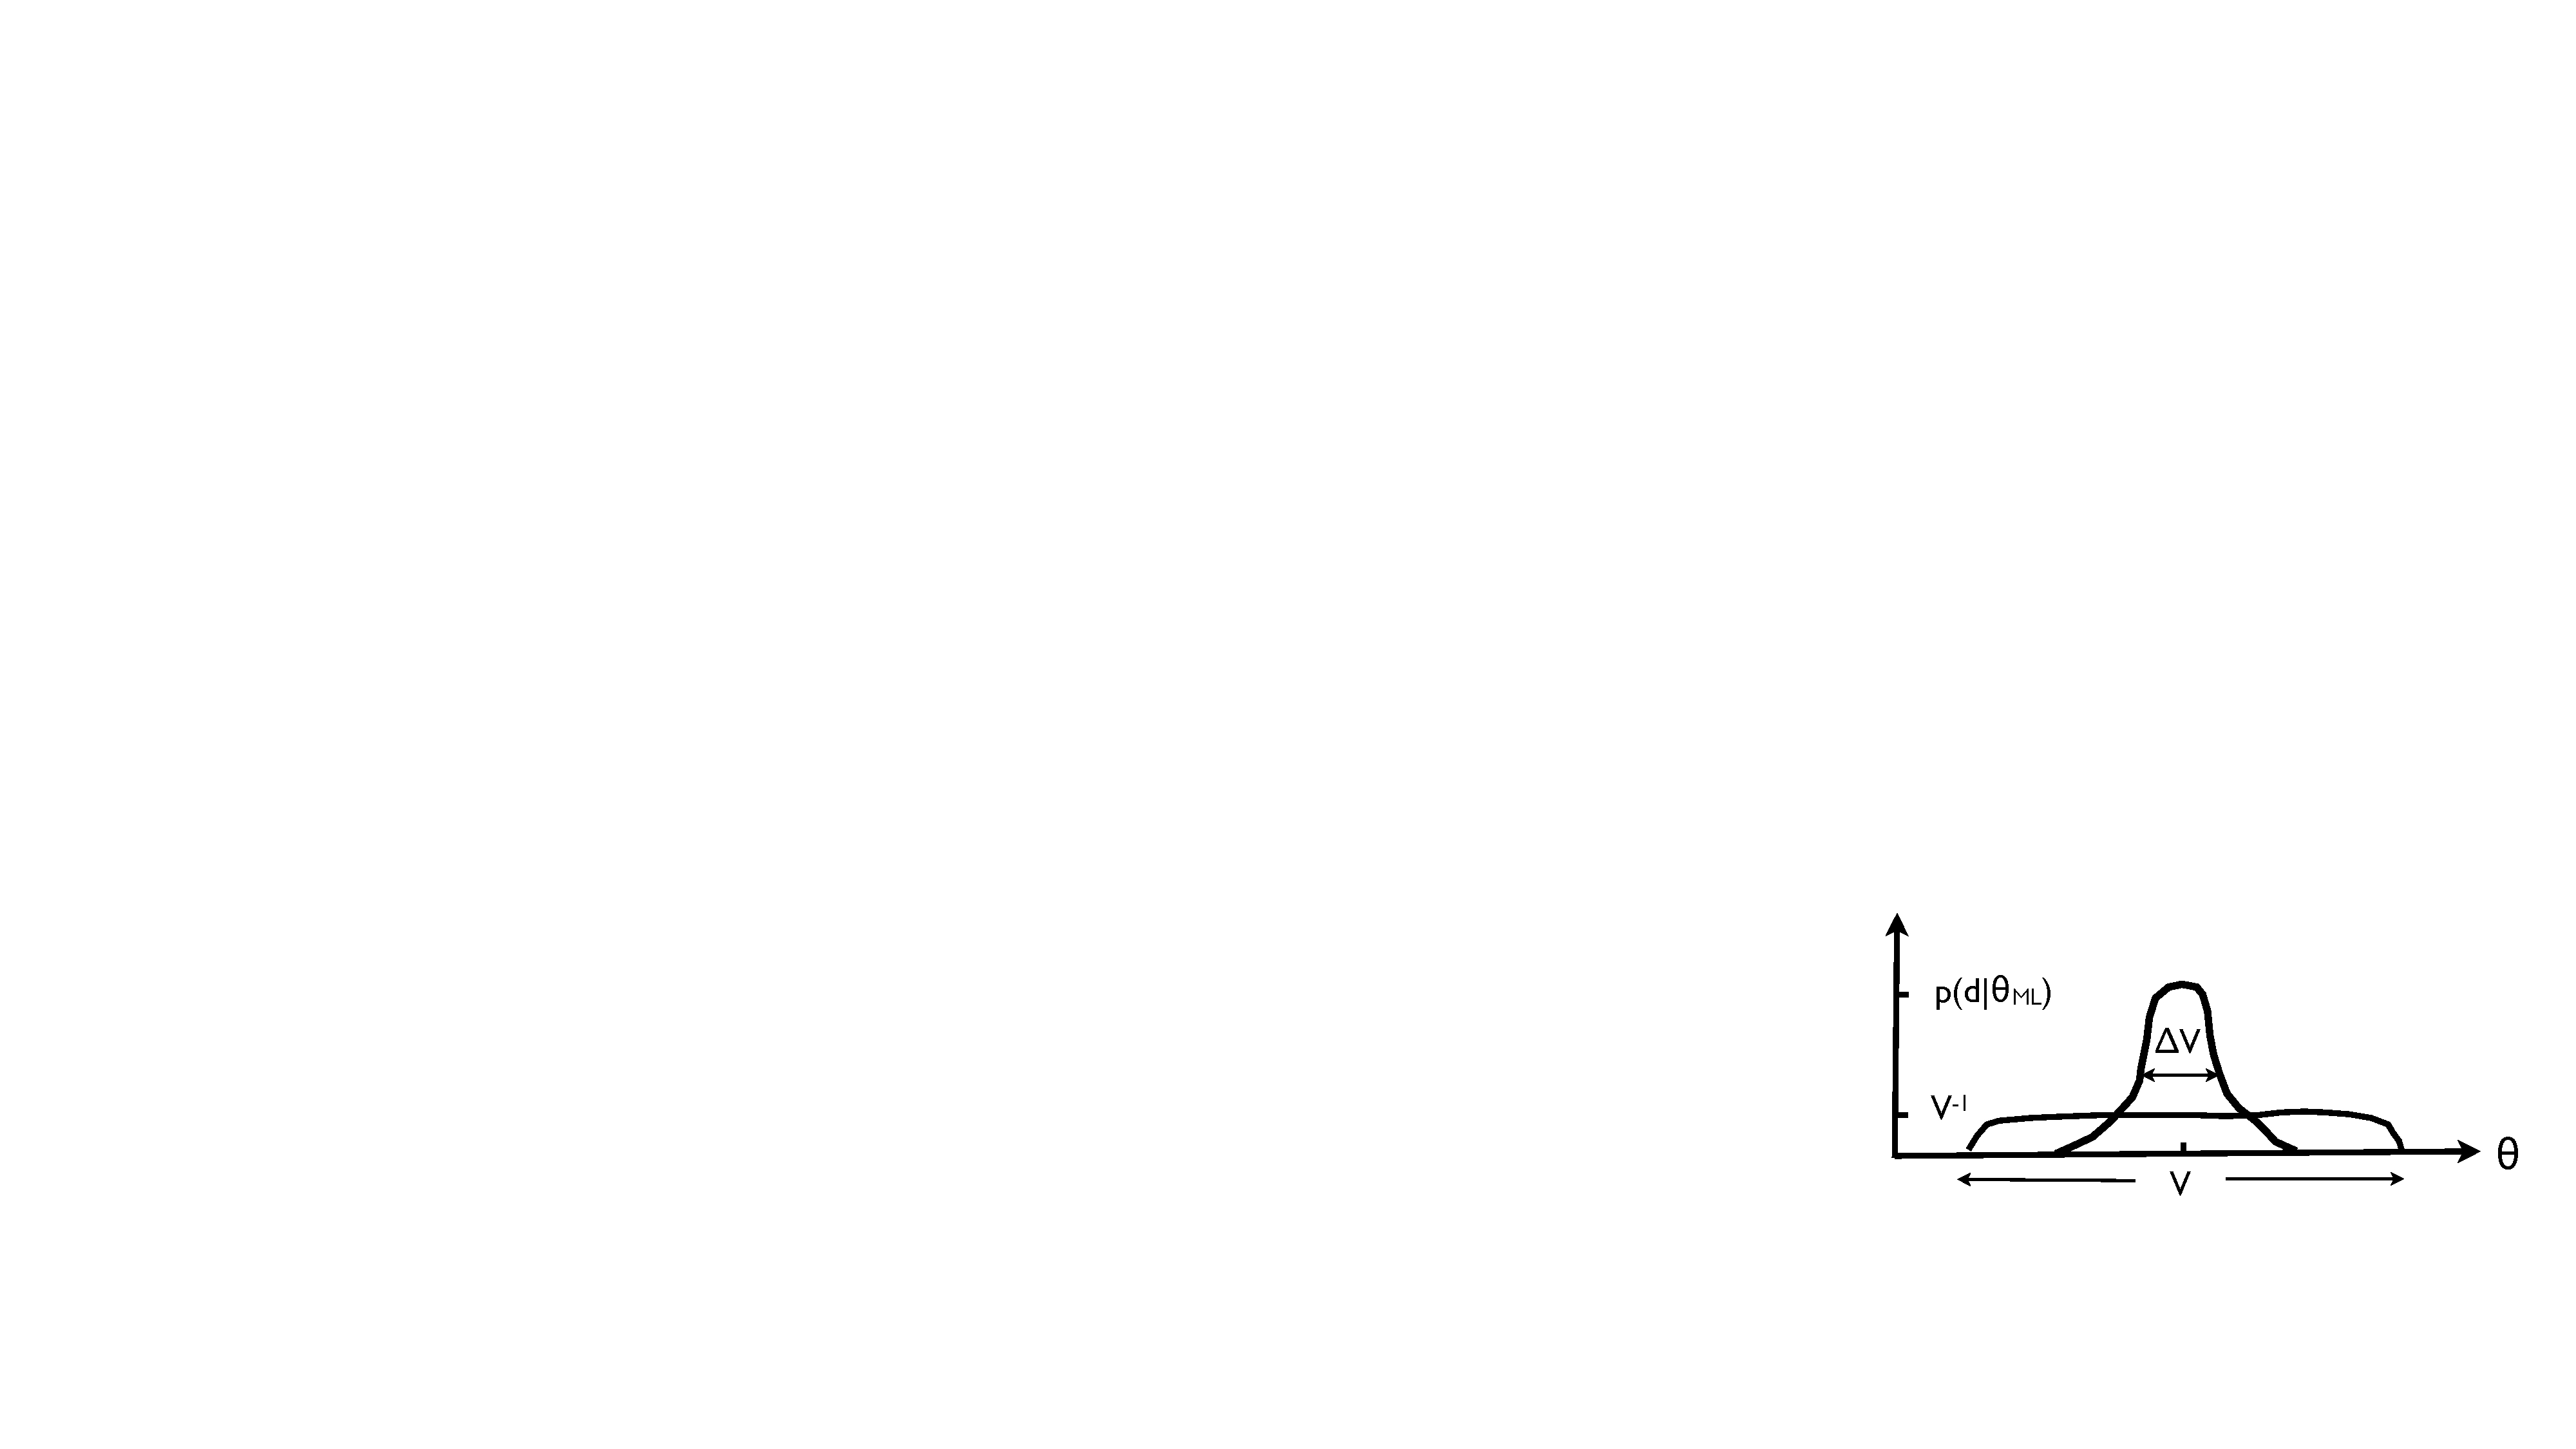
\includegraphics[width=0.45\textwidth]{Figures/informative_data}
\caption{Schematic representation of the likelihood function
and prior probability distribution for a parameter $\theta$,
when the data $d$ are informative.
In this case, thelikelihood function is peaked relative to the 
prior probability distribution, with maximum at 
$\theta=\theta_{\rm ML}$ and characteristic width $\Delta V$.
The parameter space volume is denoted by $V$.}
\label{f:informative_data}
\end{center}
\end{figure}

\begin{figure}[htbp!]
\begin{center}
\subfigure[]{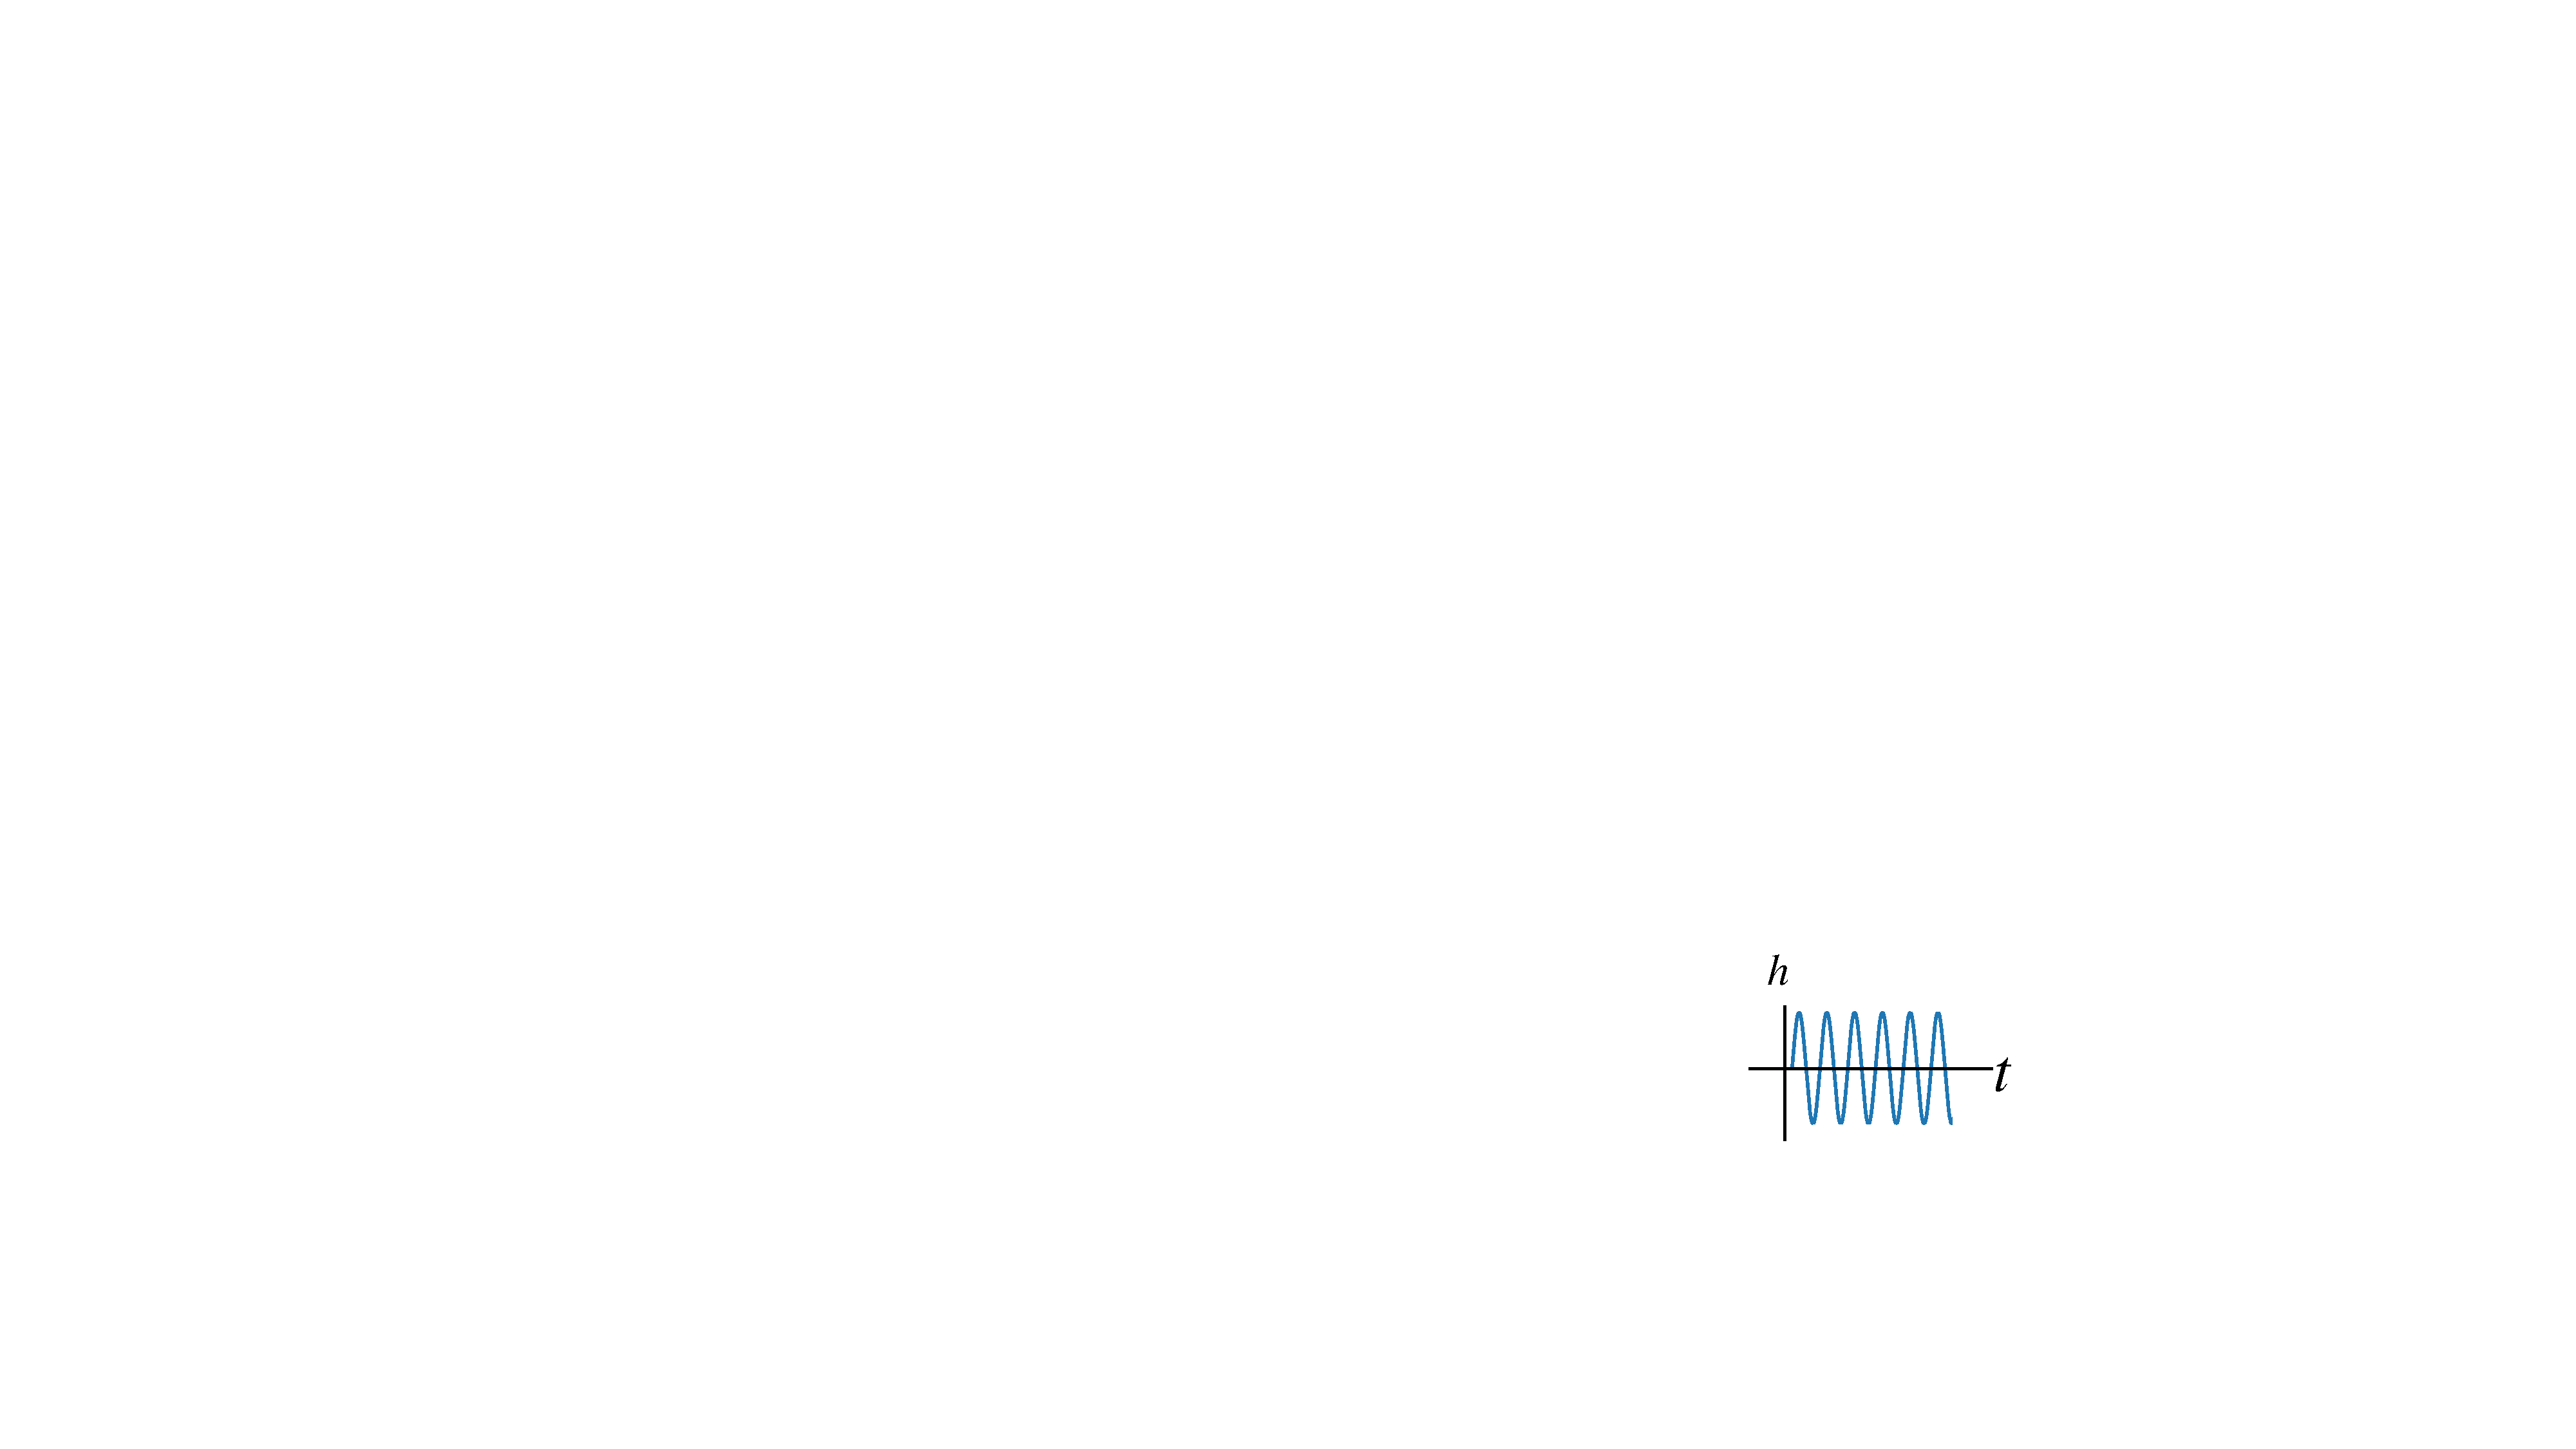
\includegraphics[width=0.25\textwidth]{Figures/sinusoid_prior}}
\hspace{1 in}
\subfigure[]{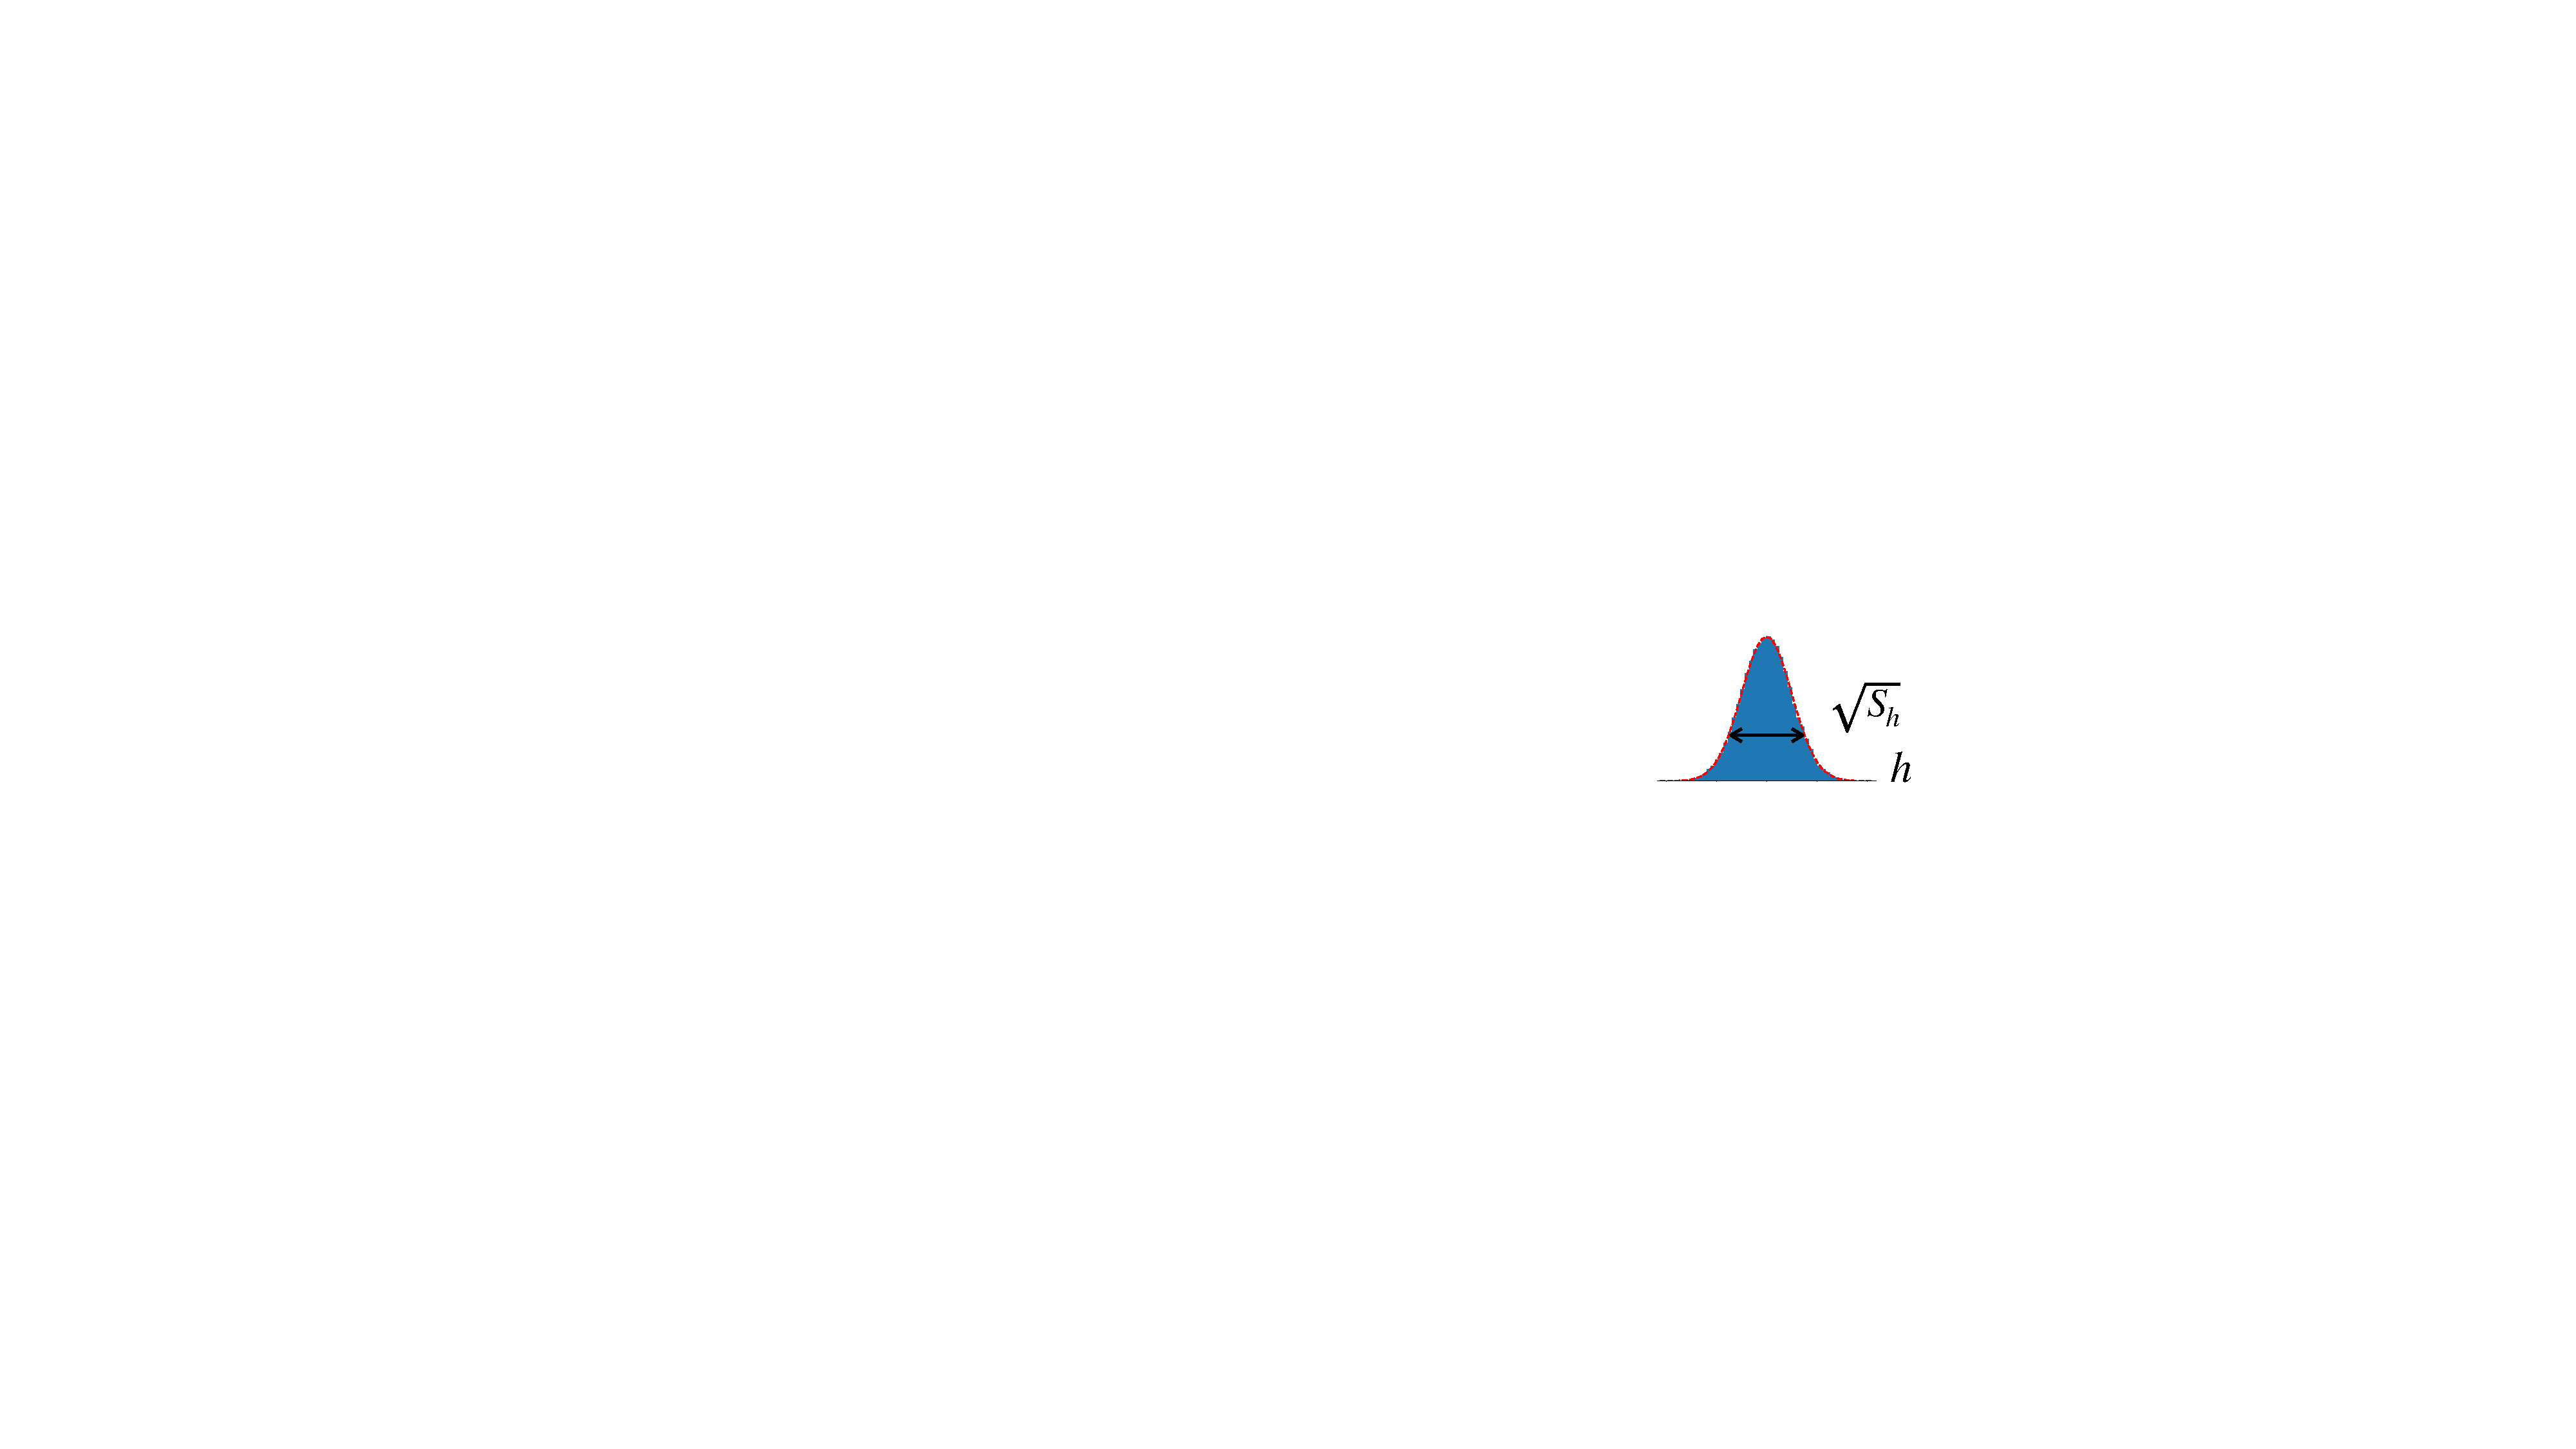
\includegraphics[width=0.25\textwidth]{Figures/stochastic_prior}}
\caption{Different signal priors for $h(t)$.
Panel (a): Determinsitic (sinusoid) signal prior.
Panel (b): Stochastic signal prior.
For the stochastic signal prior, $h(t)$ values are drawn from a
Gaussian distribution with variance $S_h$.}
\label{f:det_stoch_signal_priors}
\end{center}
\end{figure}

%%%%%%%%%%%%%%%%%%%%%%%%%%%%%%%%%%%%%%%%%%%%%%%%%%%%%%%
\section{Searching for the background of binary black-hole
mergers}
\label{s:nonstationary}

\begin{figure}[htbp!]
\begin{center}
\subfigure[]{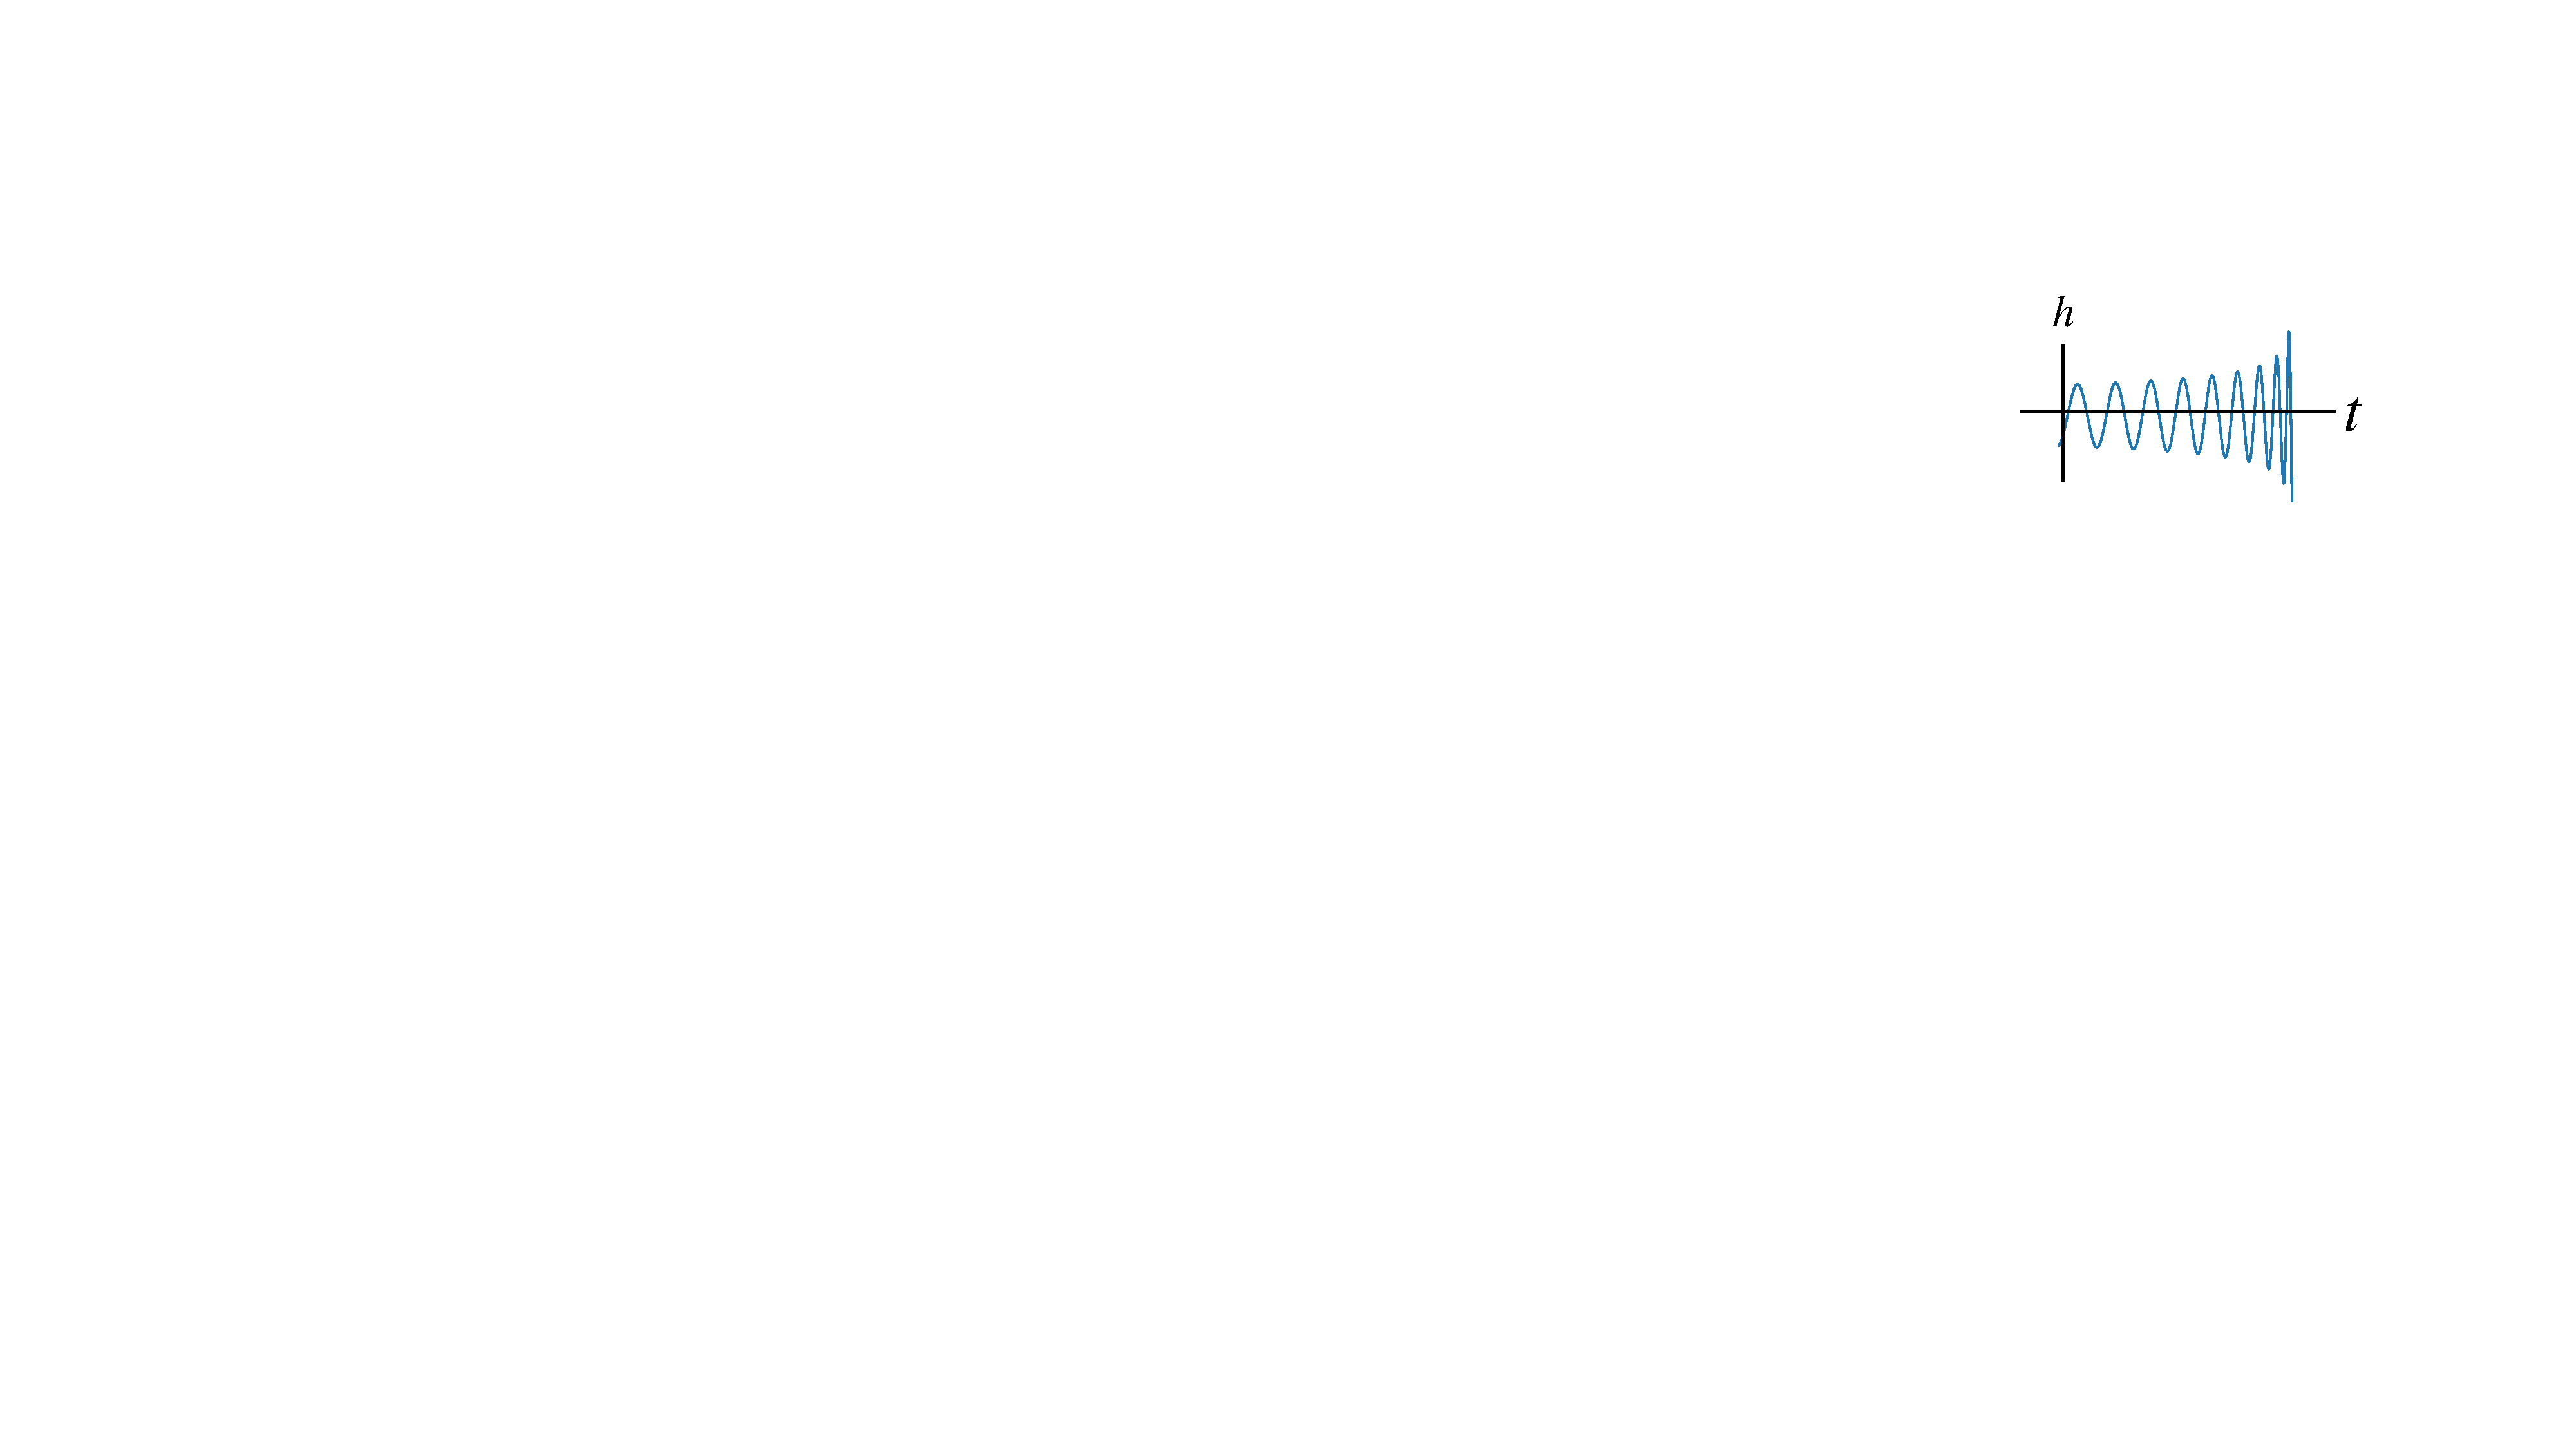
\includegraphics[width=0.25\textwidth]{Figures/chirp_prior}}
\hspace{1 in}
\subfigure[]{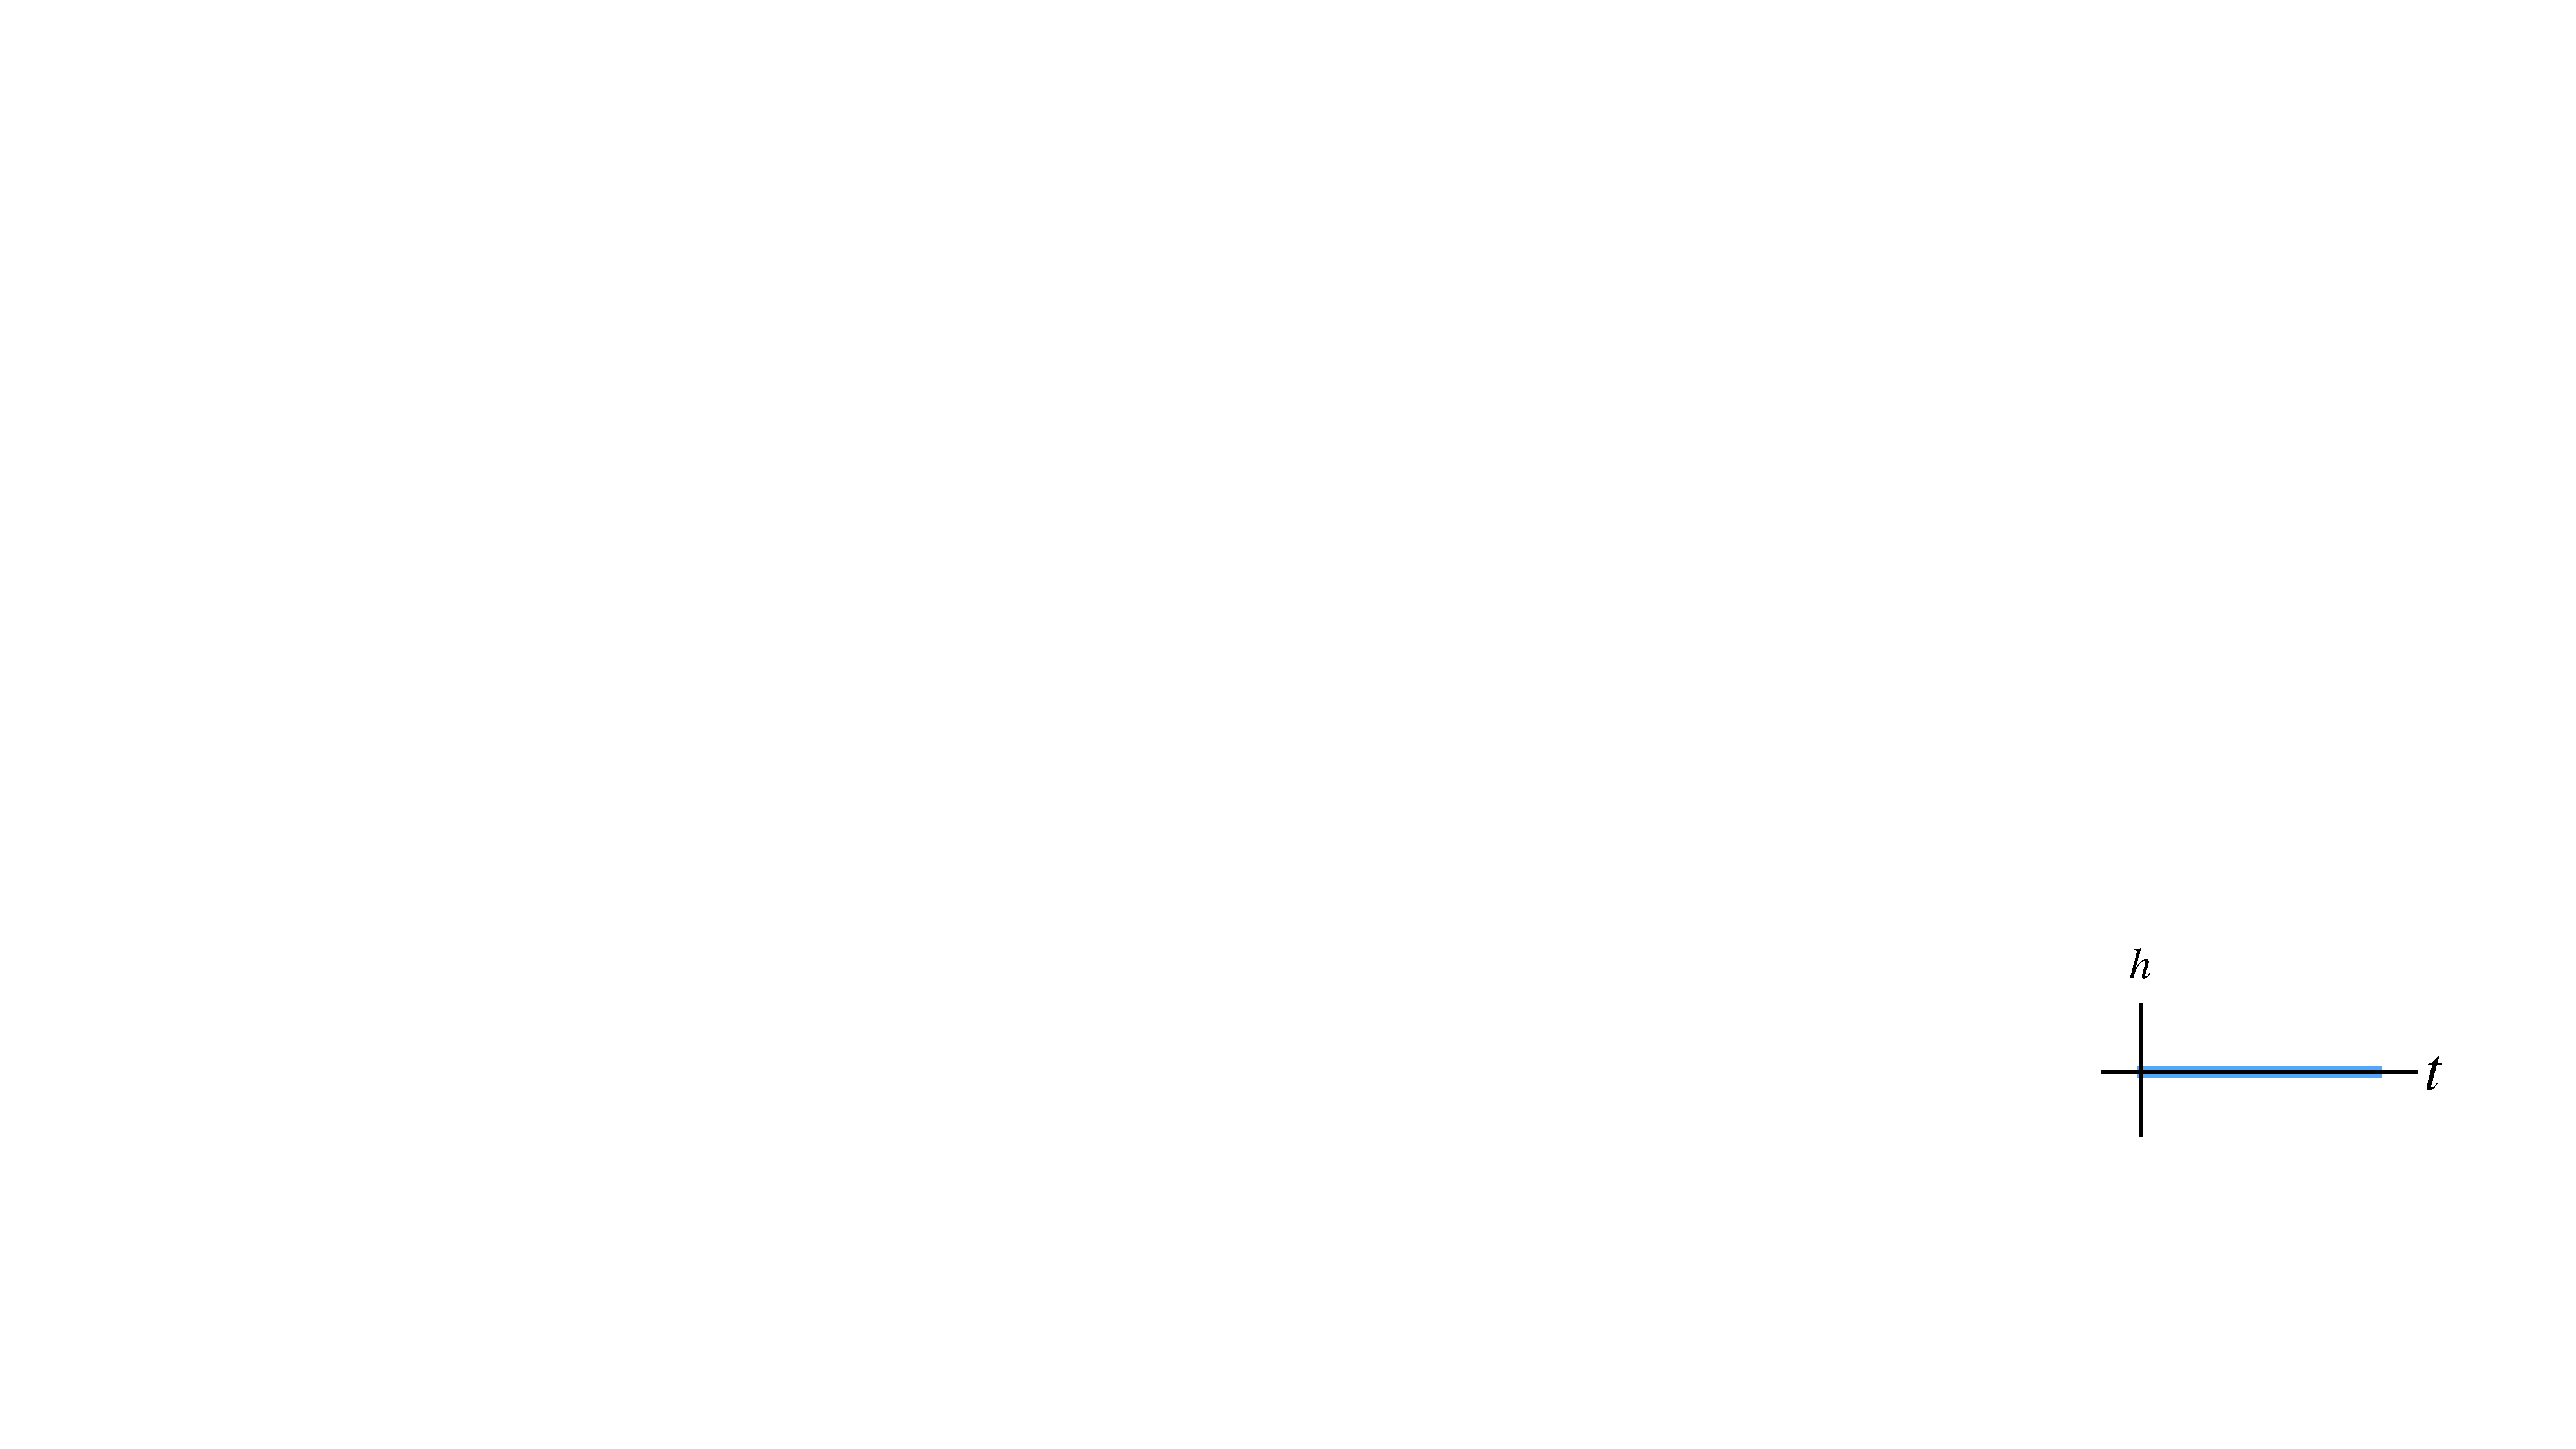
\includegraphics[width=0.25\textwidth]{Figures/no_signal_prior}}
\caption{The two components of the ``mixture" signal prior for the Bayesian 
BBH search.
Panel (a): With probability $\xi$, the signal prior for $h(t)$ is a 
chirp waveform.
Panel (b): With probability $(1-\xi)$, the signal prior for $h(t)$ is that
the signal is absent, i.e., $h(t)=0$.}
\label{f:mixture_signal_priors}
\end{center}
\end{figure}

\begin{figure}[htbp!]
\begin{center}
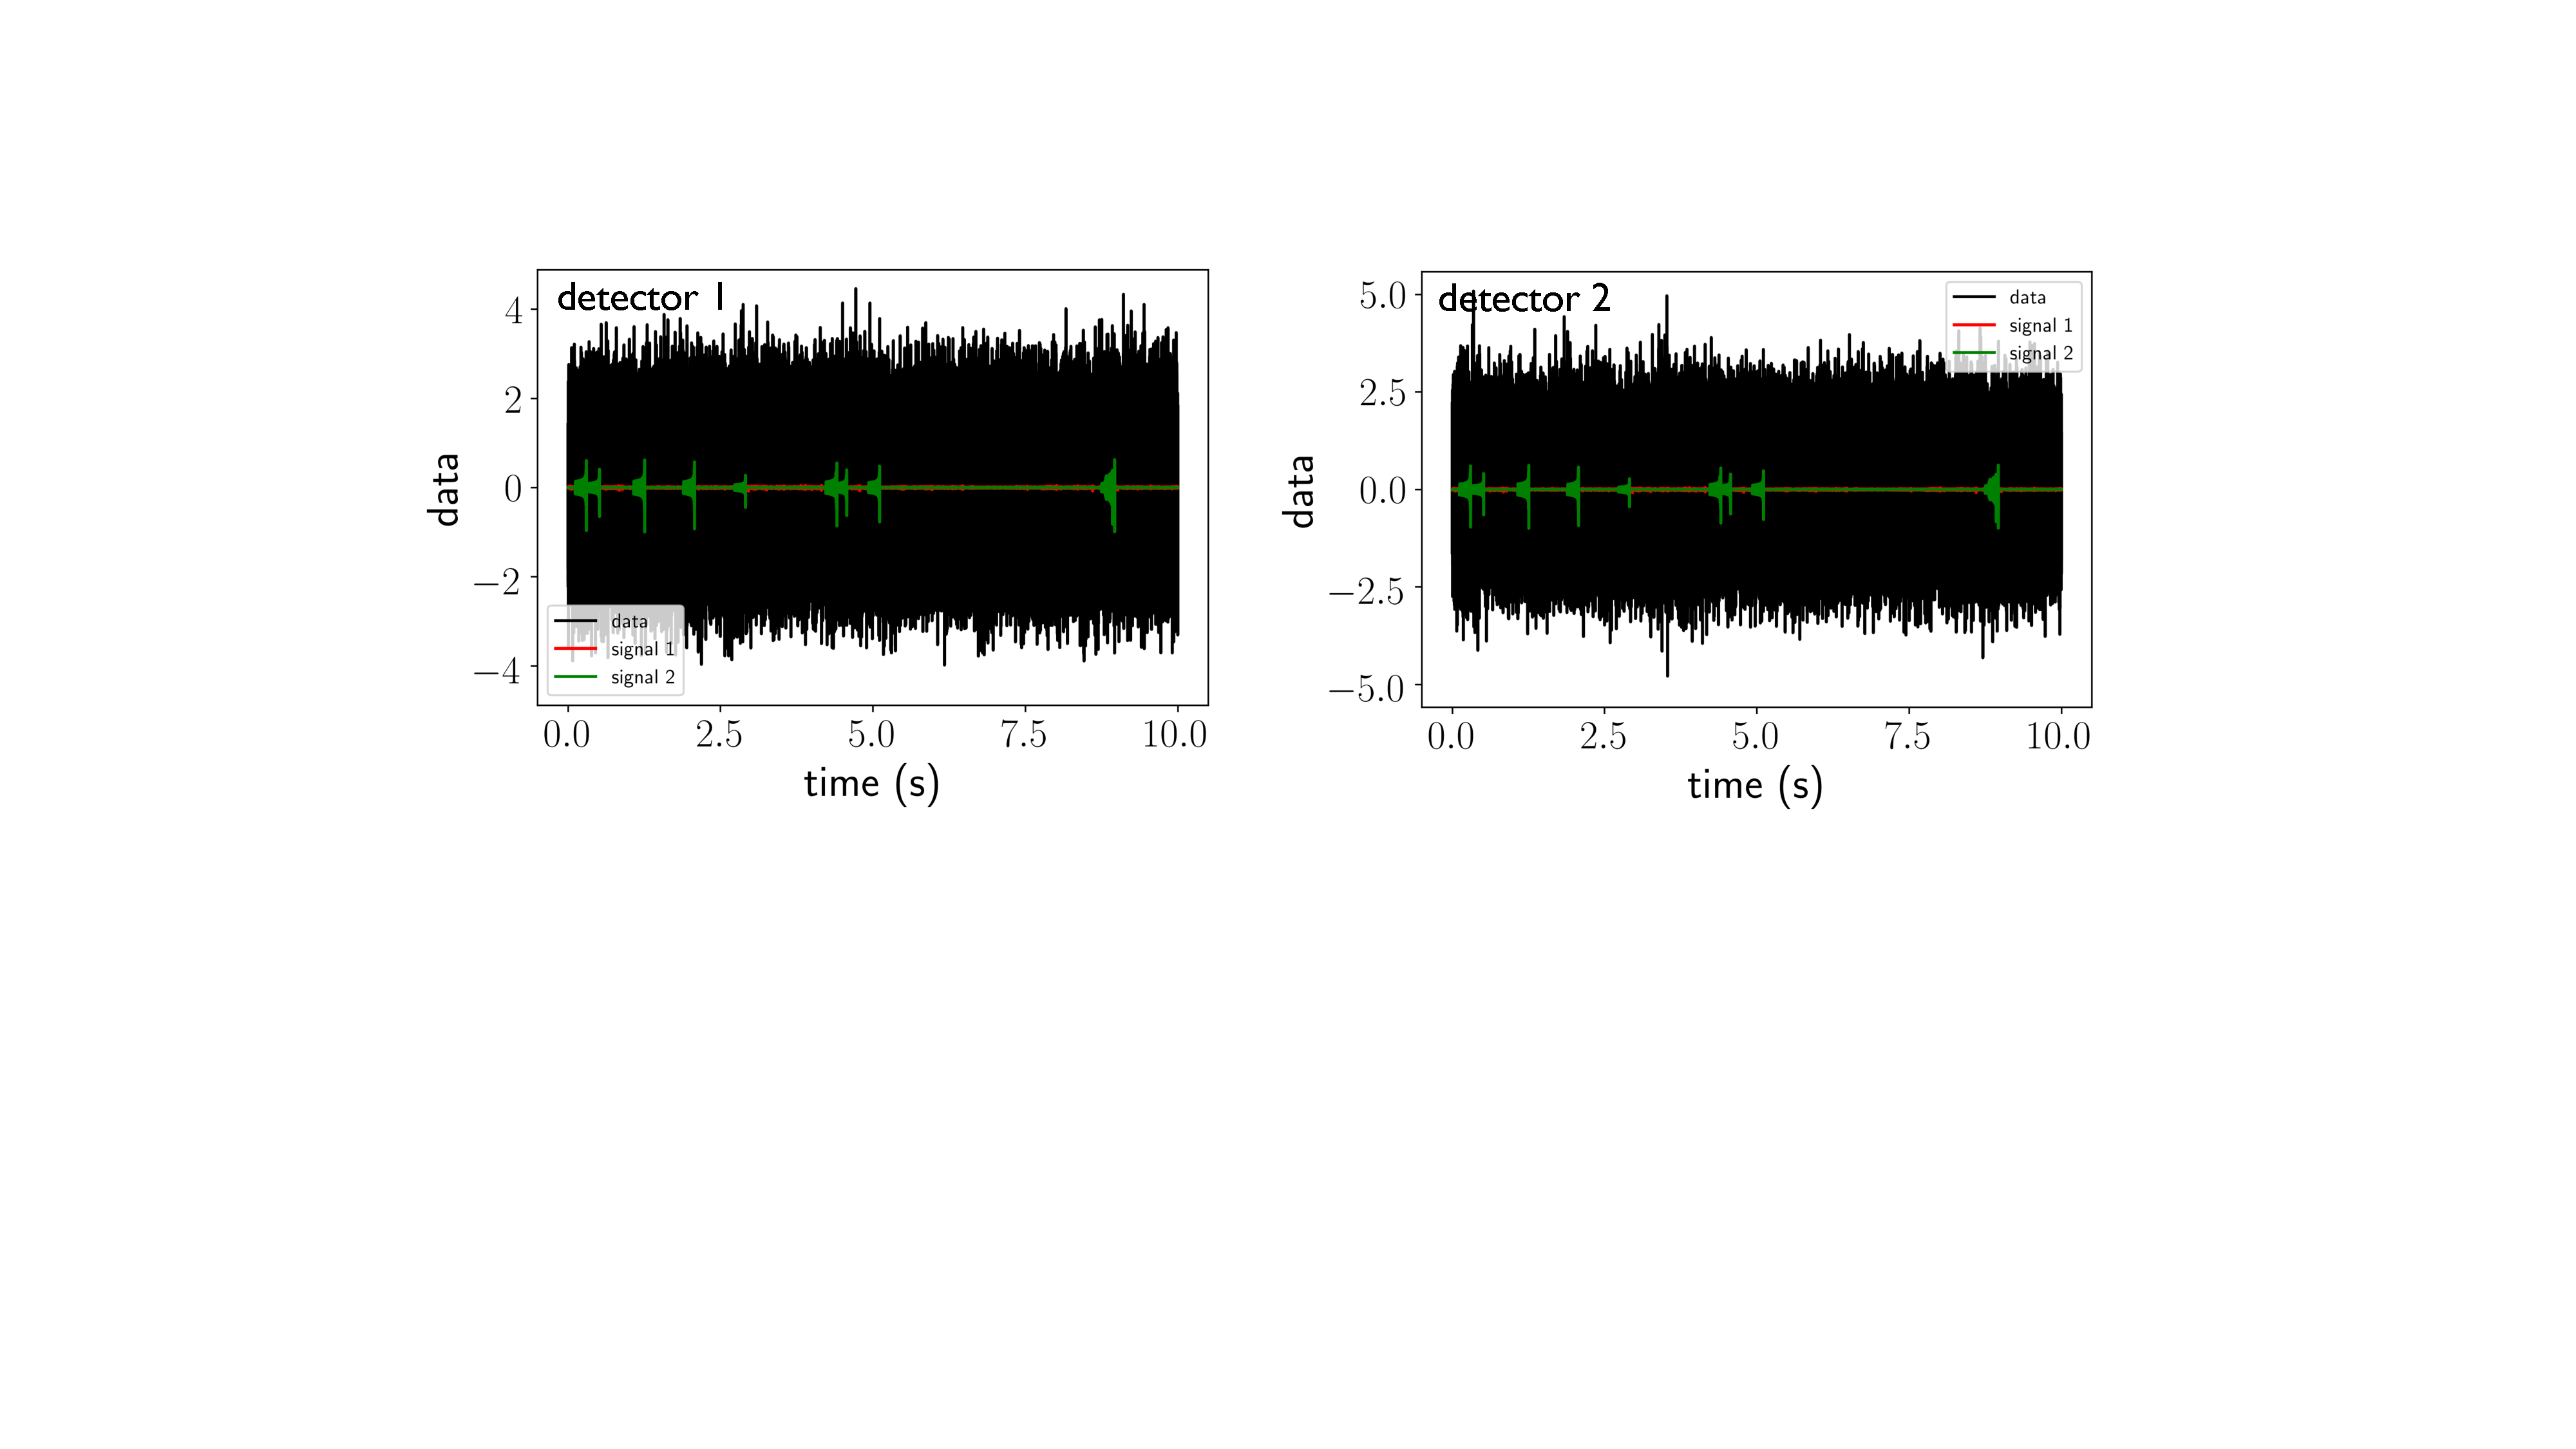
\includegraphics[width=\textwidth]{Figures/BBH-BNS-simulated-data}
\caption{Simulated BBH and BNS data in two coincident and coaligned
detectors.
The confusion-limited BNS background is shown in orange;
the popcorn-like BBH background is shown in green.
The black trace is the data consisting of the BBH and BNS signal
plus white Gaussian-stationary noise, uncorrelated in the two
detectors.}
\label{f:BBH-BNS-simulated-data}
\end{center}
\end{figure}

\begin{figure}[htbp!]
\begin{center}
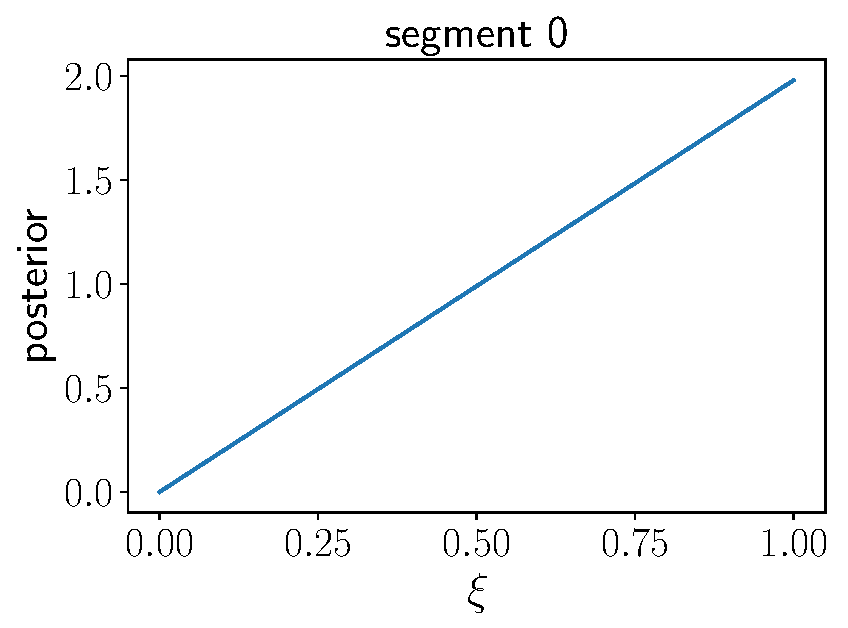
\includegraphics[width=0.24\textwidth]{Figures/posterior_xi_seg_0}
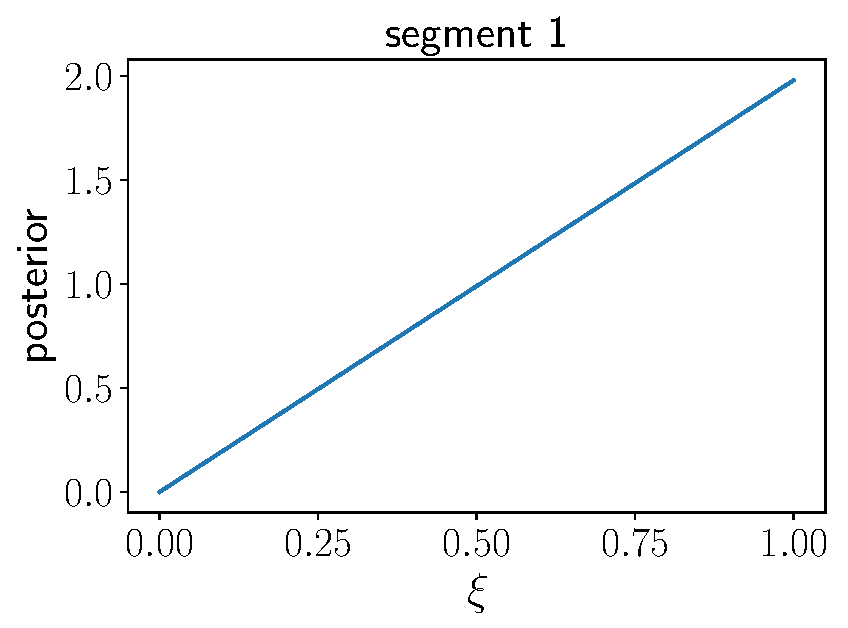
\includegraphics[width=0.24\textwidth]{Figures/posterior_xi_seg_1}
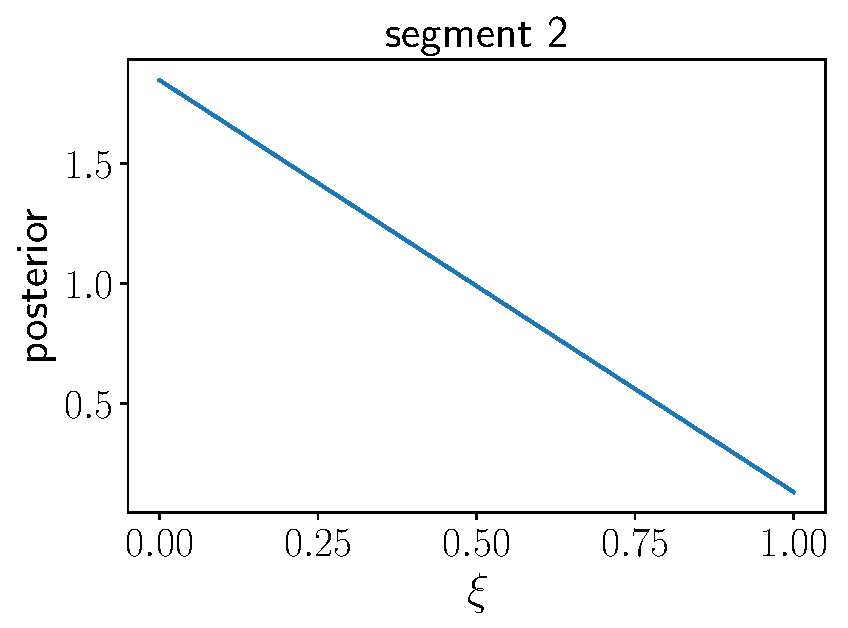
\includegraphics[width=0.24\textwidth]{Figures/posterior_xi_seg_2}
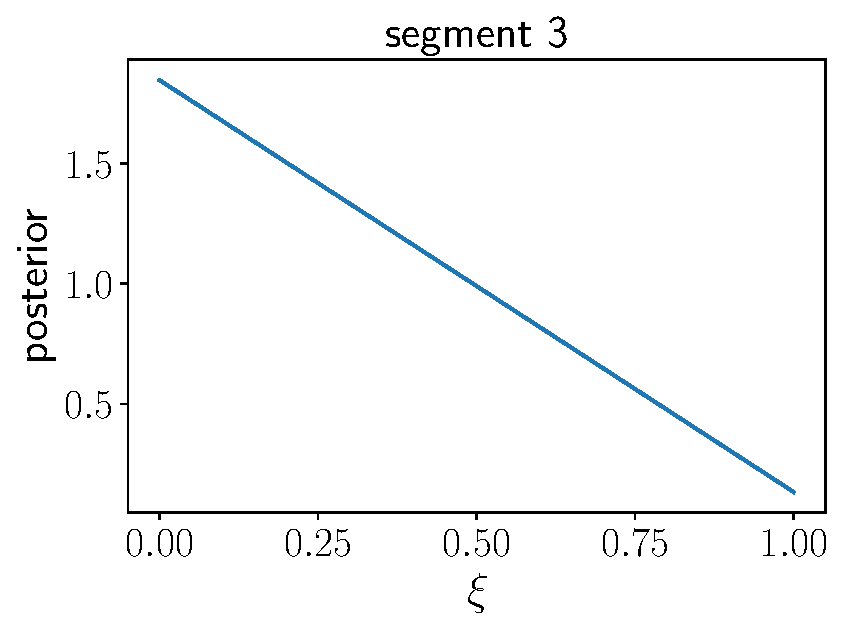
\includegraphics[width=0.24\textwidth]{Figures/posterior_xi_seg_3}
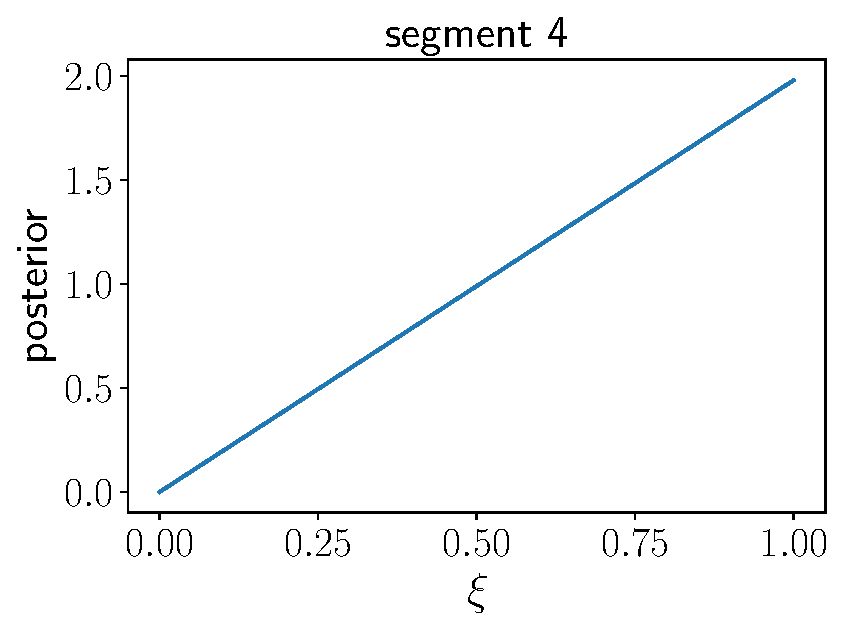
\includegraphics[width=0.24\textwidth]{Figures/posterior_xi_seg_4}
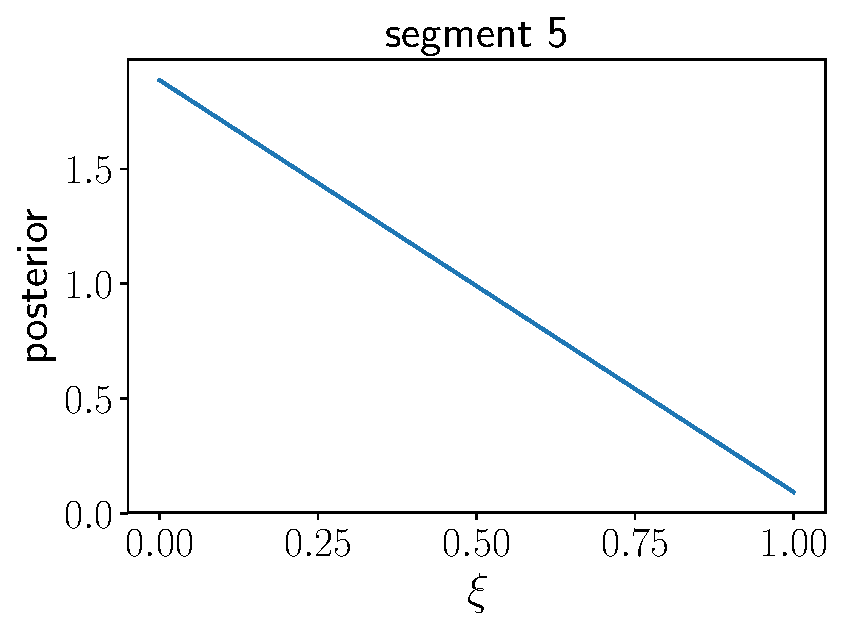
\includegraphics[width=0.24\textwidth]{Figures/posterior_xi_seg_5}
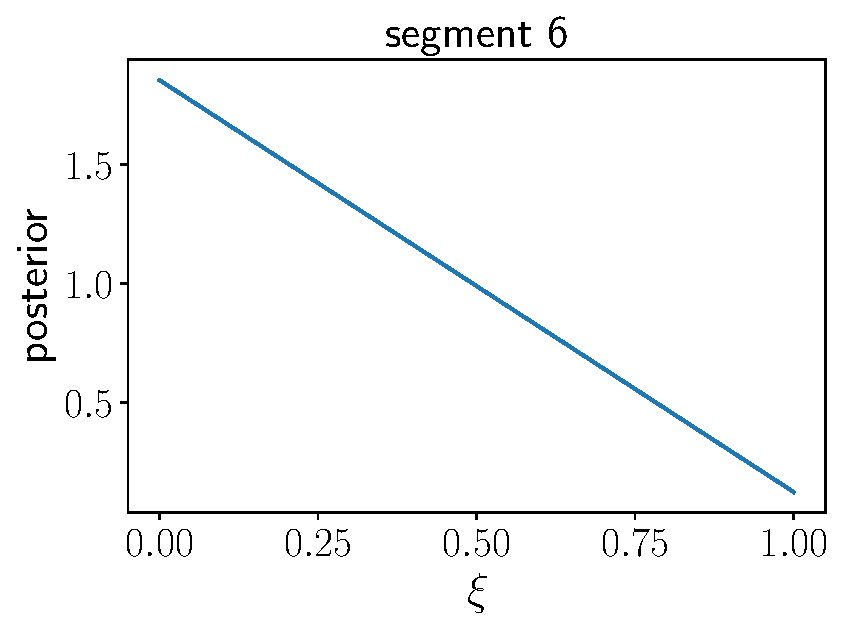
\includegraphics[width=0.24\textwidth]{Figures/posterior_xi_seg_6}
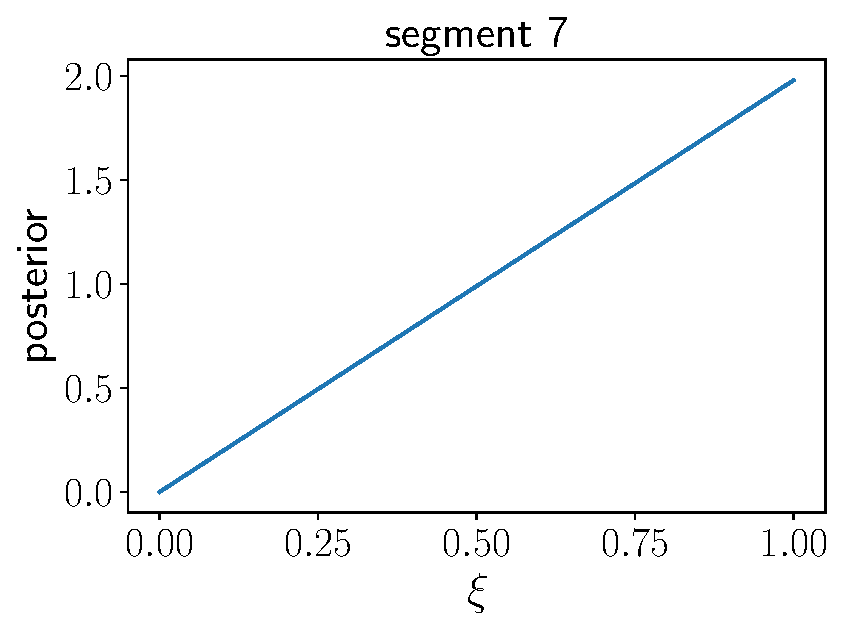
\includegraphics[width=0.24\textwidth]{Figures/posterior_xi_seg_7}
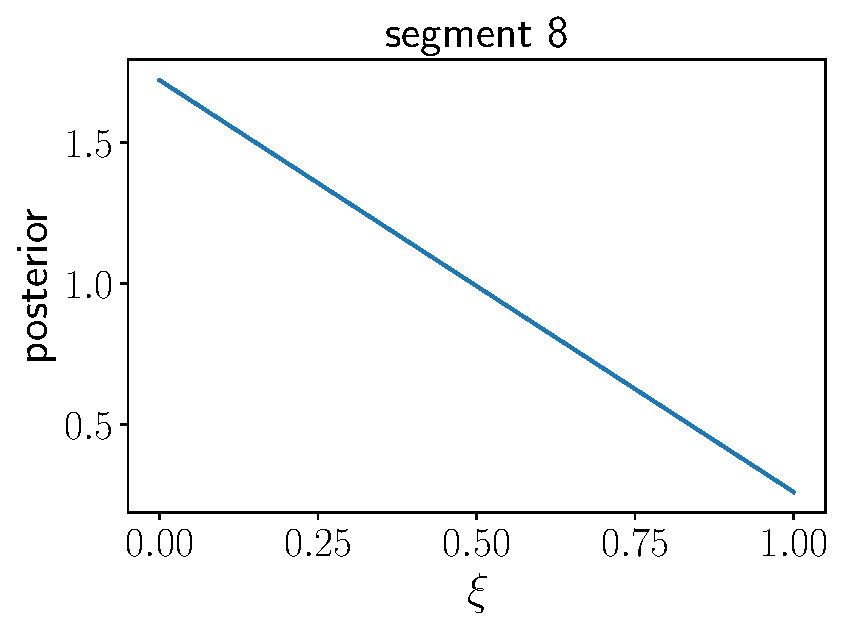
\includegraphics[width=0.24\textwidth]{Figures/posterior_xi_seg_8}
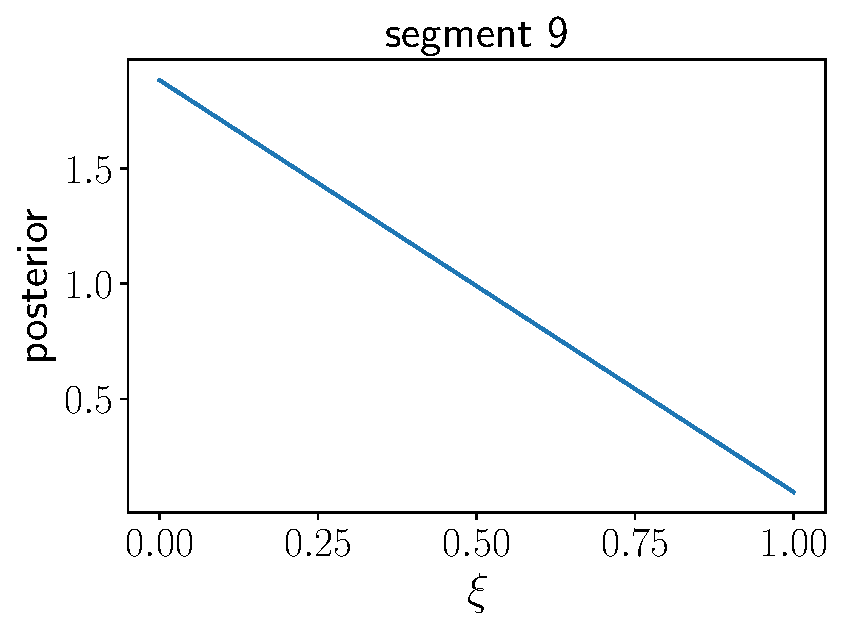
\includegraphics[width=0.24\textwidth]{Figures/posterior_xi_seg_9}
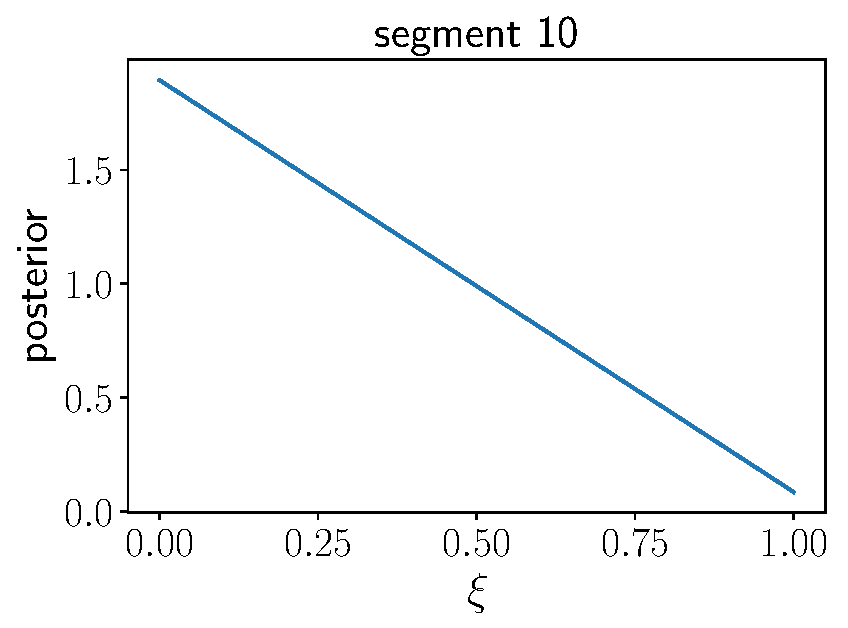
\includegraphics[width=0.24\textwidth]{Figures/posterior_xi_seg_10}
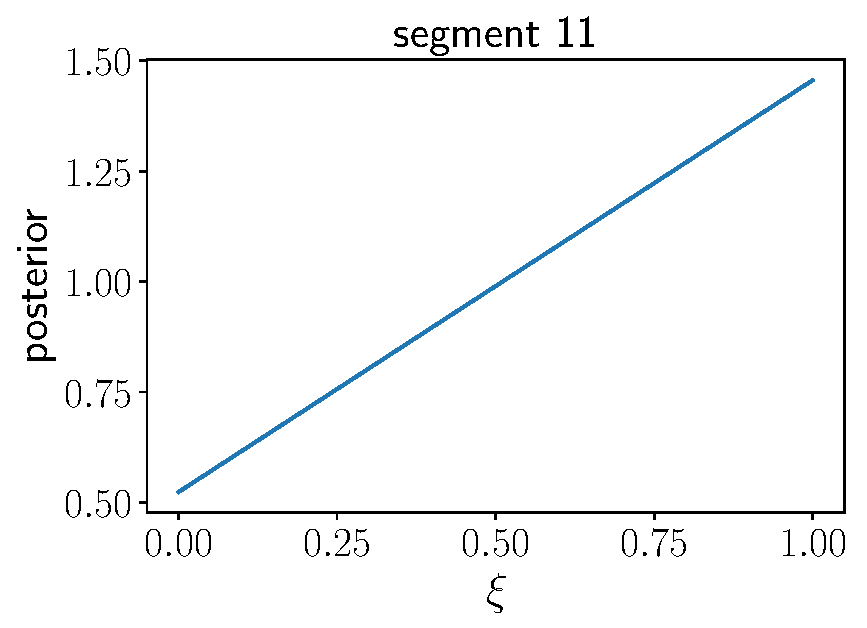
\includegraphics[width=0.24\textwidth]{Figures/posterior_xi_seg_11}
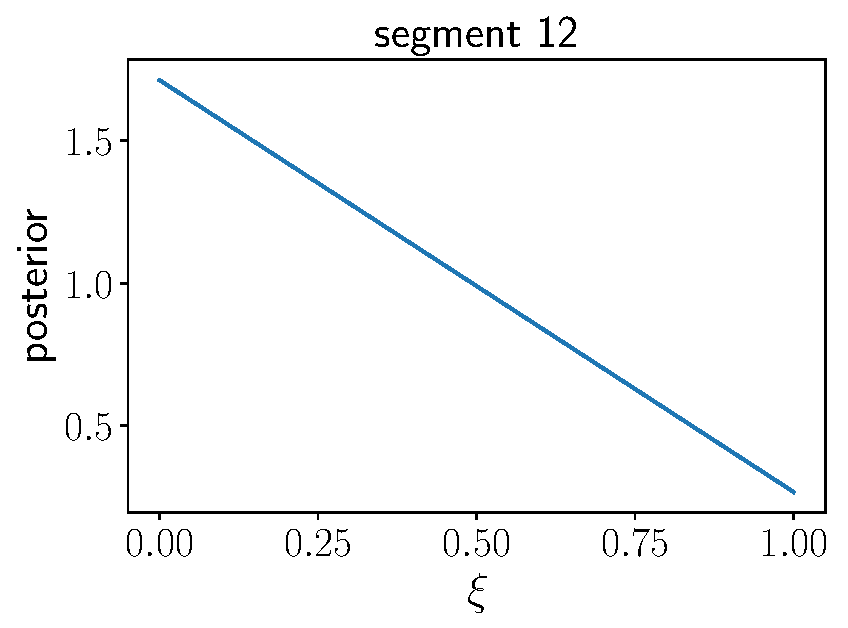
\includegraphics[width=0.24\textwidth]{Figures/posterior_xi_seg_12}
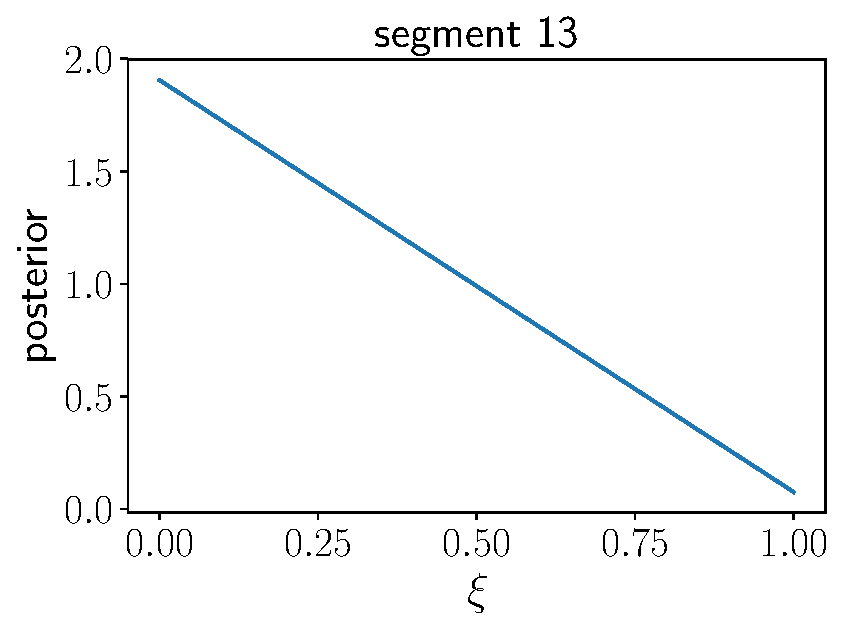
\includegraphics[width=0.24\textwidth]{Figures/posterior_xi_seg_13}
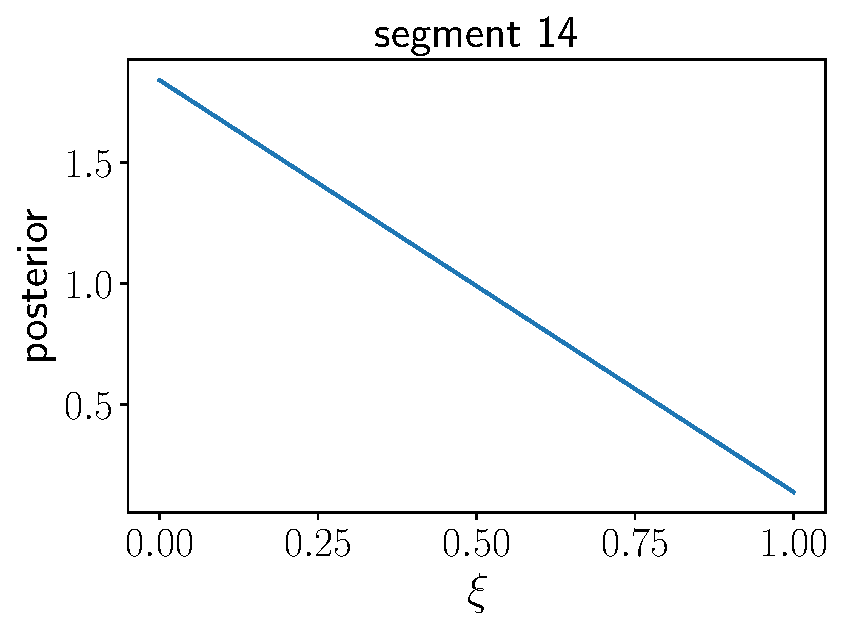
\includegraphics[width=0.24\textwidth]{Figures/posterior_xi_seg_14}
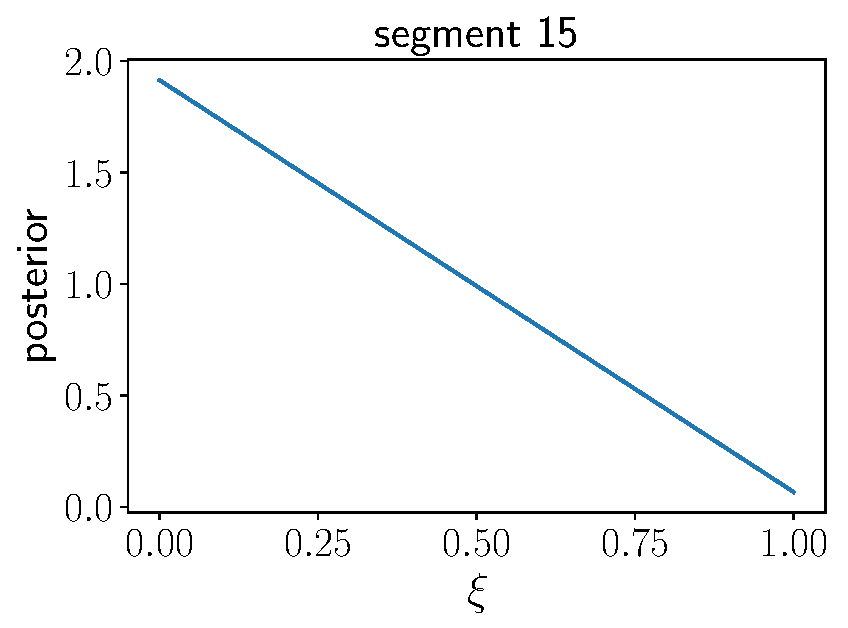
\includegraphics[width=0.24\textwidth]{Figures/posterior_xi_seg_15}
\caption{Posterior distributions for $\xi$ for the first 16 segments
(i.e., first 4~s) of data.}
\label{f:posteriors_xi_seg}
\end{center}
\end{figure}

\begin{figure}[htbp!]
\begin{center}
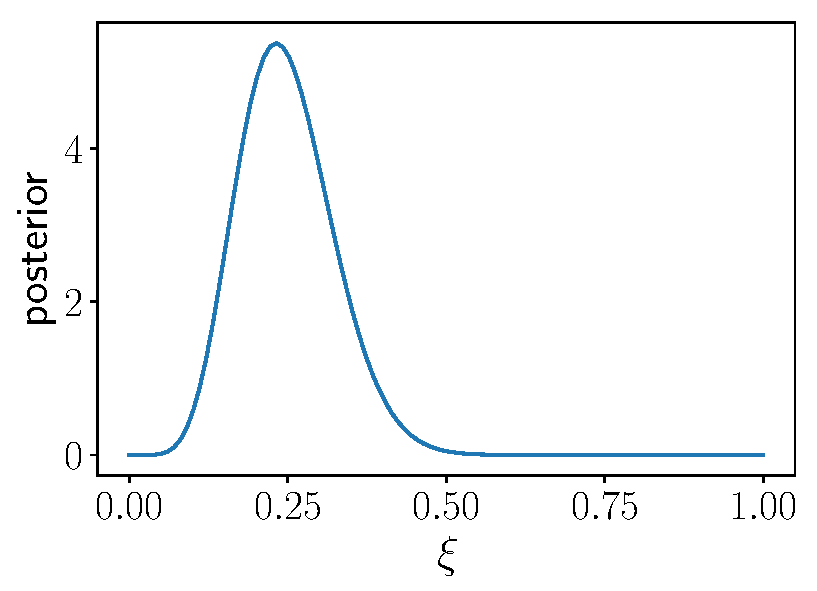
\includegraphics[width=0.5\textwidth]{Figures/posterior_xi}
\caption{The cumulative posterior distribution for $\xi$ after 
combining all 40~segments of data.}
\label{f:posterior_xi}
\end{center}
\end{figure}

\begin{figure}[htbp!]
\begin{center}
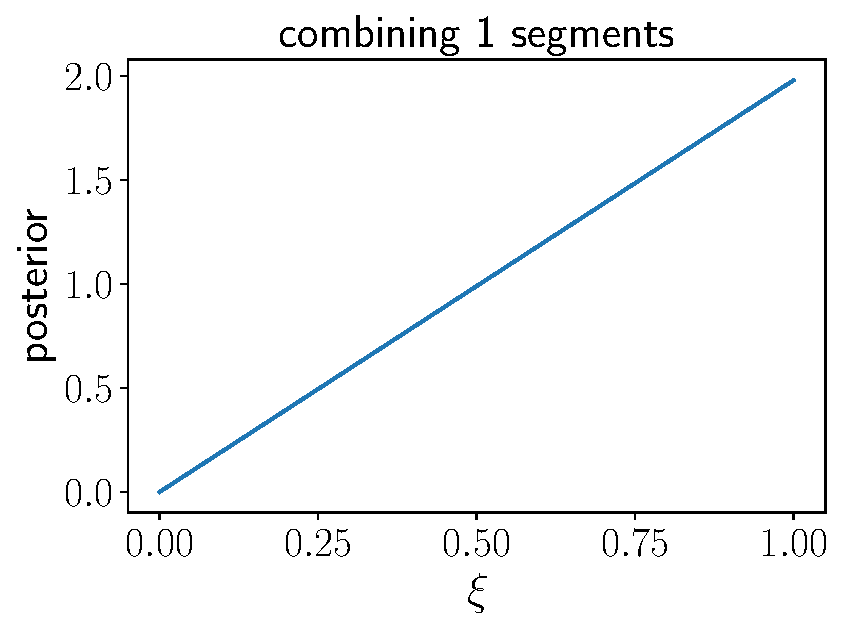
\includegraphics[width=0.24\textwidth]{Figures/posterior_xi_cum_0}
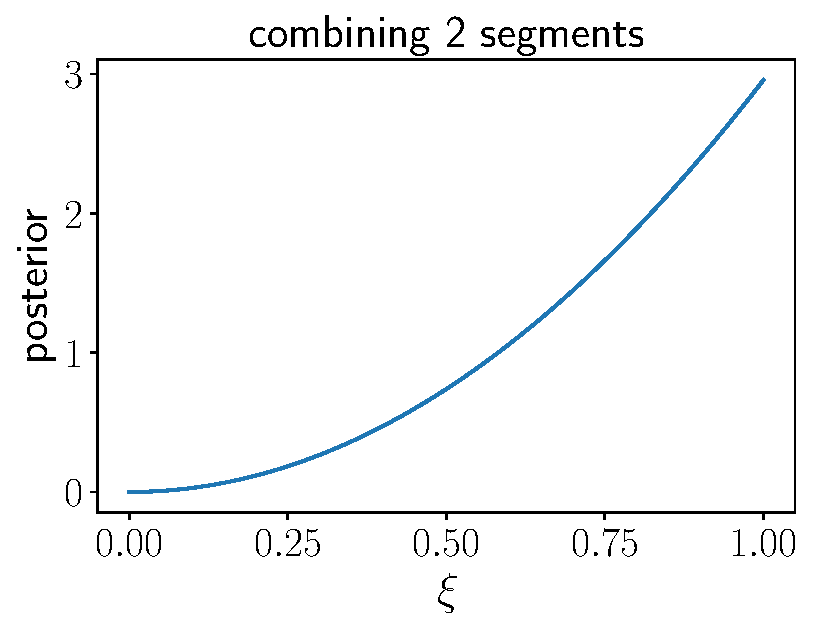
\includegraphics[width=0.24\textwidth]{Figures/posterior_xi_cum_1}
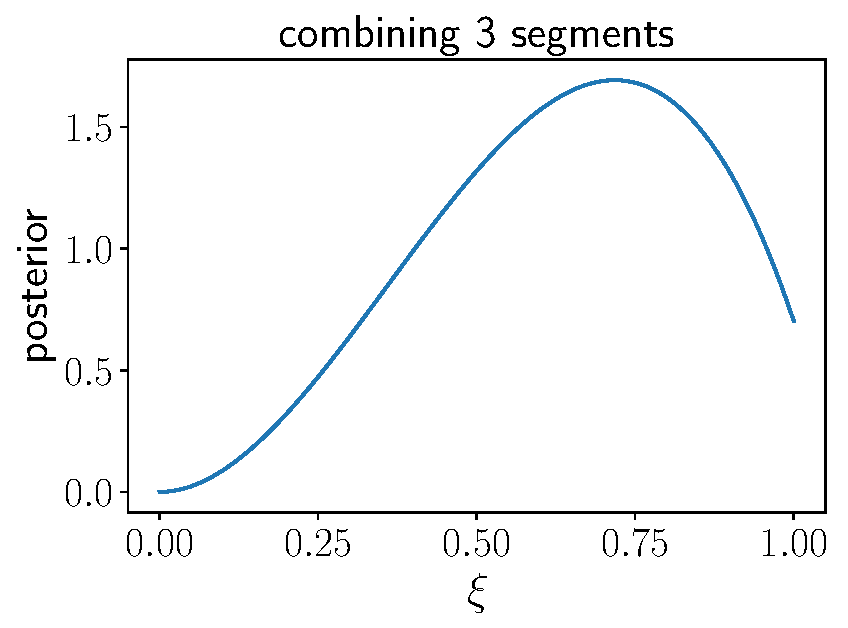
\includegraphics[width=0.24\textwidth]{Figures/posterior_xi_cum_2}
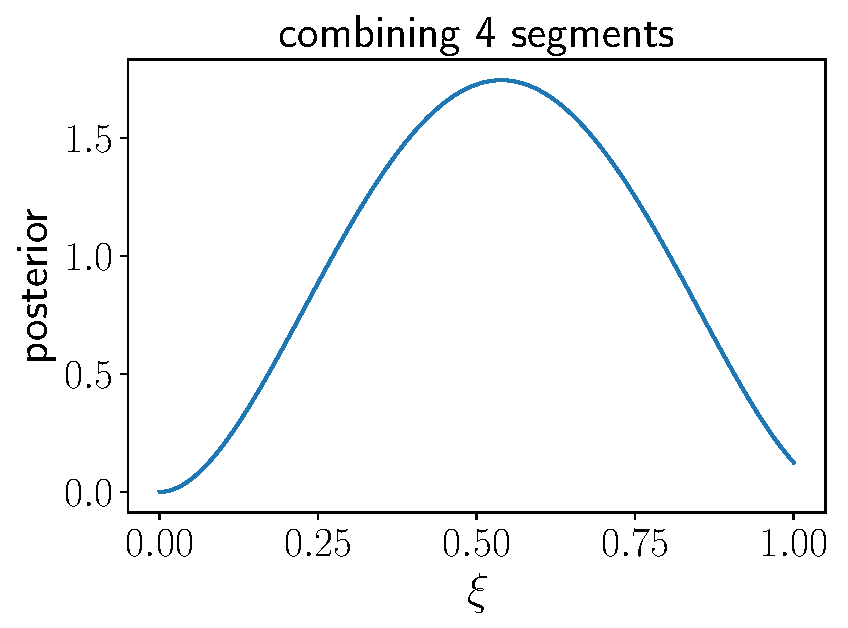
\includegraphics[width=0.24\textwidth]{Figures/posterior_xi_cum_3}
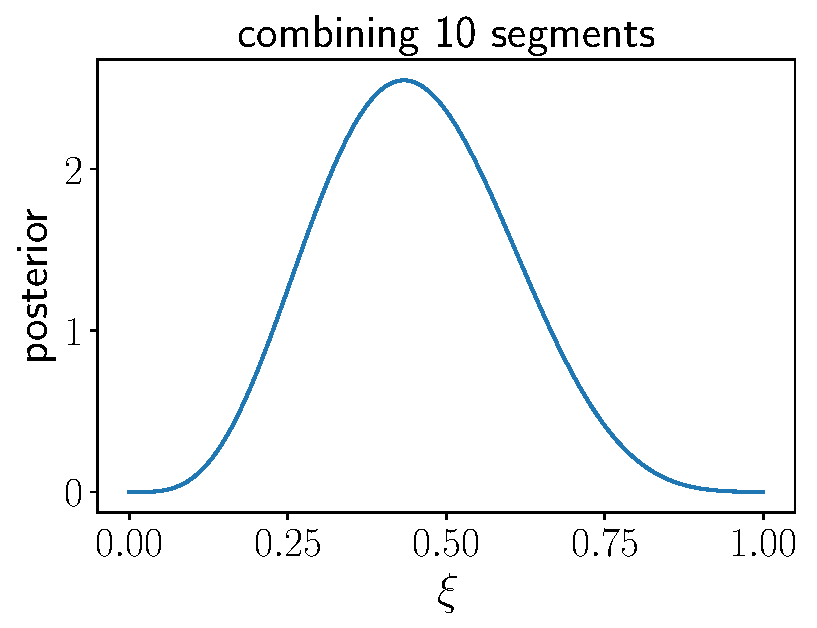
\includegraphics[width=0.24\textwidth]{Figures/posterior_xi_cum_9}
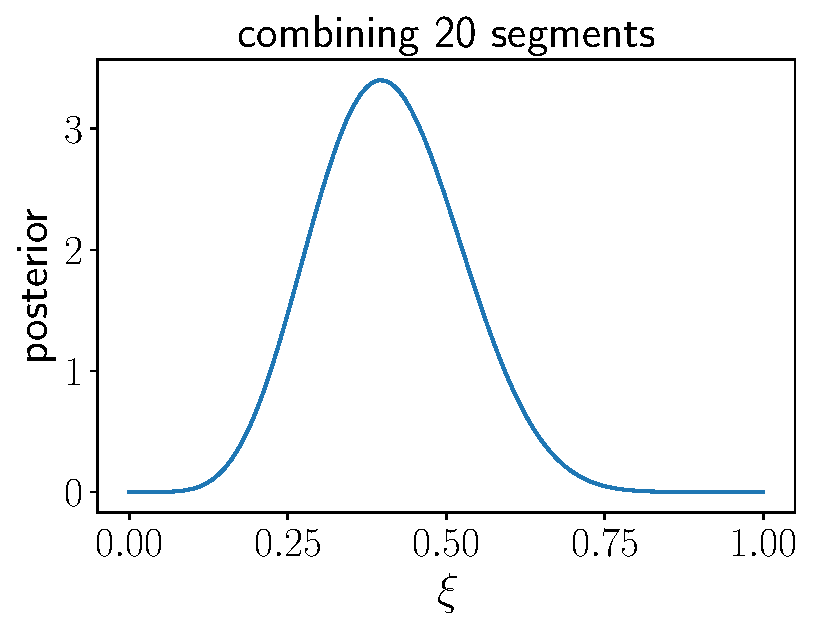
\includegraphics[width=0.24\textwidth]{Figures/posterior_xi_cum_19}
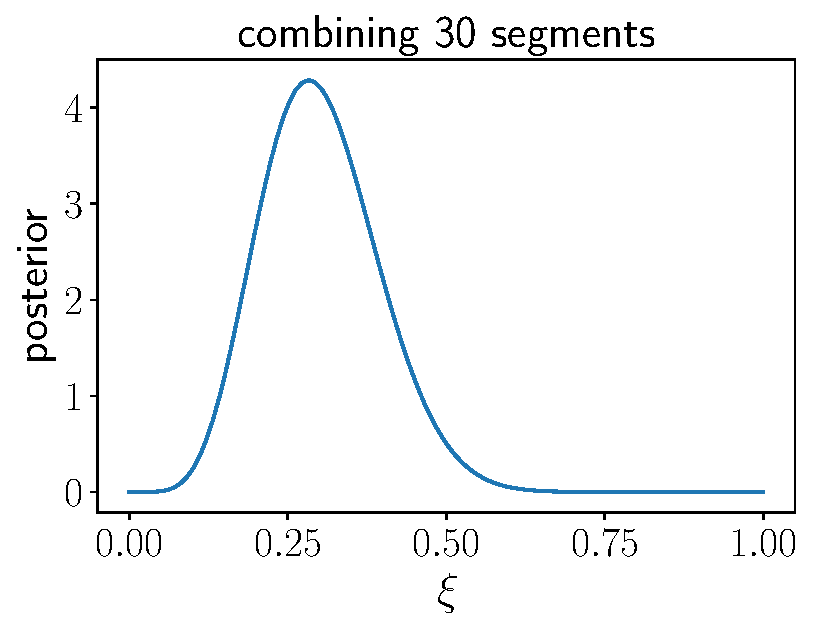
\includegraphics[width=0.24\textwidth]{Figures/posterior_xi_cum_29}
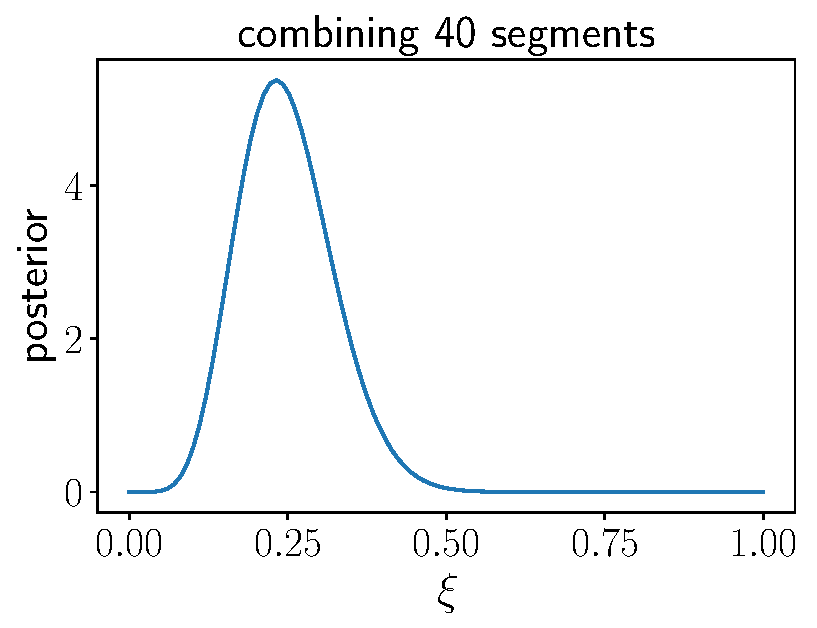
\includegraphics[width=0.24\textwidth]{Figures/posterior_xi_cum_39}
\caption{Cumulative posterior distributions for $\xi$ combining the
first $n$ segments of data.
The bottom-rightmost plot is also shown in Figure~\ref{f:posterior_xi}.}
\label{f:posteriors_xi_cum}
\end{center}
\end{figure}


